\documentclass[english,11pt,a4paper,oneside]{report}
\usepackage{tcolorbox}
\usepackage{alltt}
\usepackage[english]{babel}
\usepackage[T1]{fontenc}
\usepackage[utf8]{inputenc}
\usepackage{lmodern}
\usepackage{amsmath}
\usepackage{amsfonts}
\usepackage{amssymb}
\usepackage{graphicx}
\usepackage{float}
\usepackage{subcaption}
\usepackage{listings}
\usepackage{longtable}
\usepackage{tabularx}
\usepackage{tabulary}
\usepackage{booktabs}
\usepackage{multirow}
\usepackage{paralist}
\usepackage[inline]{enumitem}
\usepackage[authoryear,round,sort&compress]{natbib}
\usepackage[font=small,labelfont=bf,format=hang]{caption}
\usepackage[left=3cm,right=3cm,top=2.5cm,bottom=2.5cm]{geometry}
\usepackage{fancyhdr}
\usepackage{hyperref}

\renewcommand{\bibsection}{\chapter*{References}}
\parindent0pt
\renewcommand{\baselinestretch}{1.05}
\setlength{\parskip}{6pt}

\captionsetup[table]{name=Tab.}
\captionsetup[figure]{name=Fig.}
\renewcommand{\figurename}{\footnotesize Fig.}
\renewcommand{\tablename}{\footnotesize Tab.}
\renewcommand{\contentsname}{Contents}
\renewcommand{\listfigurename}{List of Figures}
\renewcommand{\listtablename}{List of Tables}
\renewcommand{\chaptername}{Chapter}
\renewcommand{\appendixname}{Appendix}

\renewcommand{\thefigure}{\arabic{chapter}-\arabic{figure}}
\renewcommand{\thetable}{\arabic{chapter}-\arabic{table}}
\renewcommand{\theequation}{\arabic{chapter}-\arabic{equation}}
\counterwithin{figure}{chapter}
\counterwithin{table}{chapter}
\counterwithin{equation}{chapter}

\pagestyle{fancy}
\fancyhf{}
\cfoot{\thepage}
\lhead{ZHAW LSFM}
\chead{Bachelor Thesis}
\rhead{Etienne Dürig}

\hypersetup{%
	colorlinks=true,
	citecolor=blue,
	linkcolor=blue,
	urlcolor=blue,
	anchorcolor=blue}
	
	
\fancypagestyle{plain}{
	\fancyhf{}
	\renewcommand{\headrulewidth}{0pt}
	\renewcommand{\footrulewidth}{0pt}
}

\begin{document}
	% Titelseite, ZHAW, Standard

\begin{titlepage}
	
	% Logo, rechts ausrichten 
	\begin{flushright}
		
\includegraphics[width=0.15\textwidth]{Bilder/logo-zhaw.png}
	\end{flushright}

\begin{center}

\vspace*{1cm} % Abstand nach dem Logo, anpassen nach Bedarf

	% Nachfolgende Informationen zentriert auf der Seite
	\Large \textsc{Zurich University of Applied Sciences} \\ 
	\vspace{0.15cm}
	\Large \textsc{Department Life Science and Facility Management} \\
	\vspace{0.15cm}
	\Large \textsc{Institute for Computational Life Sciences}
	
	\vspace{1cm}

	% Titel der Arbeit
	\Large \textbf{Sensitivity Analysis of a TIR-Based Cold-Water Patch Detection Algorithm
	}
	
	\textbf\\
	 The Influence of Cold Water Tributaries on Cold Water Patches

	\vspace{1cm}
	
	% Art der Arbeit und Vertraulichkeit
	\large Bachelor Thesis\\
	%\vspace*{0.15cm}
	% \large (Vertraulich)
	
	\vspace{0.5cm}

	% Autor(en) und Studiengang etc.
	\large by\\
	\large Dürig Etienne\\
	\vspace{0.75cm}
	
	\large Bachelor program Applied digital Life Sciences \\
	\large Focus Digital Environment\\
	\large Study cohort 2023\\
	\vspace{0.5cm}
	
	\large \today \\

\end{center}

\vfill % füllt Raum nach unten auf, so dass alles auf eine Seite passt


\large \textbf{Dr. Manuel Antonetti}\\
\large ZHAW Life Sciences und Facility Management\\
Institute for the Environment and Natural Resources\\
Research Group: Ecohydrology \\
Campus Grüenthal, 8820 Wädenswil

\large \textbf{Dr. Norman Juchler} \\
\large ZHAW Life Sciences und Facility Management\\
Institute for Computational Life Sciences\\
Research Group: Medical Image Analysis and Data Modeling\\
Schloss, 8820 Wädenswil
	
\end{titlepage}

	\newpage
	\tableofcontents
	\newpage
	\listoffigures
	\newpage
	\listoftables
	\newpage
	\chapter{Introduction}


Thermal heterogenity in river systems is a vital component of aquatic biodiversity. Specifically, the presence of cold-water refugia is essential for the survival of thermally sensitive fish species, as river temperatures in Switzerland are expected to rise due to climate change. Currently there is no comprehensive and extensive information about the presence, scale and location of such cold-water patches in water bodies available in Switzerland. This data, however, is critical for river management in the context of climate change \citep{tonolla_thermische-kartographie_2026, tonolla_tonolla_etal_2021_schlussbericht_zhaw_thermoemme_2021}



As part of a cantonal project aiming to quantify the temperature heterogenity and detect cold-water patches in the Emme River and its tributaries, TIR imagery covering over a 100 km river transect where collected in a helicopter-based survey. These  TIR images where then processes to extract longitudinal and transveral temperature gradients, as well as to detect cold-water spots. The current processing workflow involves stitching highly overlapping TIR images into orthophotos and performing thermal corrections using in-situ temperature loggers. Then, longitudinal and transversal temperature gradients are derived. Additionally, a newly developed algorithm for the automatic detection of cold-water patches is deployed with the goal of mapping these patches.


The current method for the automated detection of cold-water patches (CWPs) relies on four externally configured hyperparameters: step length, buffer width, temperature delta , and minimum area. Sensitivity analyses from previous studies indicate that the detection results vary significantly based on the chosen parameter values, with step length and  having a particularly strong influence on the variance of the algorithm's output. The primary aim of this thesis is to systematically investigate the algorithm's variance with respect to its hyperparameters, specifically focusing on how tributary inflows and adjustments to the processing workflow changes interact with the variance caused by specific hyperparameters.


The algorithm defines a CWP by comparing individual pixel temperatures against a local median reference temperature calculated over a defined segment (step length). It is hypothesised that the choice of step length introduces significant variance near the inflow of tributaries. This, because cold- or warm-water tributaries introduce sharp longitudinal temperature gradients which can skew the calculation if the step size is chosen sub-optimally


Research question 1: How does the step length contribute to the algorithms variance in river sections containing a tributary with significantly differing water temperatures, compared to sections without such tributaries?

H0: The variance introduced by the step length parameter is not influenced by the presence of a tributary with a substantially different temperature.

H1: The variance introduced by the step length parameter is significantly influenced (increased or decreased) by the presence of a tributary with a substantially different temperature.


Research question 2: What adjustments could be made to the detection-algorithm to reduce variability with respect to parameters while also achieving plausible detection results?




% the two hypothesises must be stated of course
% then also the cwp algorithm must be introduced somewhere. But I assume this is better donn the theorretical backgroudn
	\chapter{Theoretical Background}

% talk about cold water patches here. What are they, why are they interesting? Especially with respect to the salmanoid fish stuff. How are they defined. What is the critigue about the definition


\section{Model Input Sensitivity Analysis}

The inputs to models can diver and are generally dependent in their structure and manyfoldness on the nature of the model itself. Under the light of sensitivity analysis however, it can be worthwhile to define, what the inputs to a model actually contains. In sensitivity analysis, everything that causes variation in the output of the model is classified as an input \citep{saltelli_global_2007}. Providing an example: If a linear regression of a target variable $Y$ is performed, then not only are the predictors $X_1, \dots, X_n$ considered as model inputs, but also the parameters $\theta_1, \dots, \theta_n$ that correspond to the predictors. So the model:

\begin{equation}
	Y = f(X_1, X_2, \theta_1, \theta_2)
	\label{eq:model_with_params}
\end{equation}

would have four parameters from the view of sensitivity analysis. 



\section{Sensitivity Analysis}

According to Saltelli et al. sensitivity analysis is ``The study of how uncertainty in the output of a model [\dots] can be apportioned to different sources of uncertainty in the model input'' \citep{saltelli_sensitivity_2004}. Sensitivity analysis provides a range of benefits. Firstly it allows the modeller to apply a strategy called ``Factor Fixing'': if the model output $Y$ is found to be independent of one or multiple parameters $\theta_i$, then these can be set to fixed constants. It may then even be possible to condense a complete submodule of a model if all parameters connected to that submodule are noninfluential, making sensitivity analysis a tool for model simplification \citep{saltelli_global_2007}. Secondly, sensitivity analysis generally improves model validity by identifying highly influential and therefore critical model components \citep{ligmann-zielinska_spatially-explicit_2013}.

\subsection{The Morris Method}

% also add to the morris method, that it is generally a method for models with an one dimensional output. Therefore when applied to models with multidimensional output, generally some spatial lumping into a scalar value has to be performed

The Morris method belongs to the group of screening methods in sensitivity analysis. These are ideal to filter a short list of important input parameters from computationally expensive models with a great number of input parameters. This can be done as these methods only require a relatively small number of model evaluations to provide sensitivity measures for the input parameters, making them a good choice when the target of the sensitivity analysis is Factor Fixing \citep{saltelli_global_2007}. As a global method, Morris explores the entire input space by varying all input parameters simultaneously across their plausible ranges, meaning that sensitivity scores reflect average behaviour across the full parameter space rather than being tied to a single point \citep{saltelli_how_2010}. The following explanation of the Morris method closely follows \citep{saltelli_global_2007} and is explained more explicitly in chapter 3 of their book.

\subsubsection{Elementary Effects and the Sampling Grid}

At the core of this introduction sits a $k$-dimensional model $Y$ with inputs $X_1, \dots, X_k$. These inputs all together can also be written in a vector $\mathbf{X}$. The model inputs are defined in the $k$-dimensional unit cube, meaning that $X_i$ can take on a value in the interval $[0,1]$. It is worth pointing out, that every model with a continuous input can be scaled to the $[0,1]$ range, which makes the unit cube a great place to define methods. In the Morris method, this input space is discretized into a grid $\Omega$. This grid features $p$ levels. 

An elementary effect of the $i$th input parameter $X_i$ is then defined as:

\begin{equation}
	EE_i = \frac{Y(X_1, X_2, \dots, X_{i-1}, X_i + \Delta, \dots, X_k) - Y(X_1, X_2, \dots, X_k)}{\Delta}
\end{equation}

Where $\Delta$ represents some step in the unit cube. $\Delta$ can be chosen from a range of different values, which are given by the set $\left\{\frac{1}{p-1}, \dots, 1 - \frac{1}{p-1}\right\}$.

\begin{figure}[h]
	\centering
	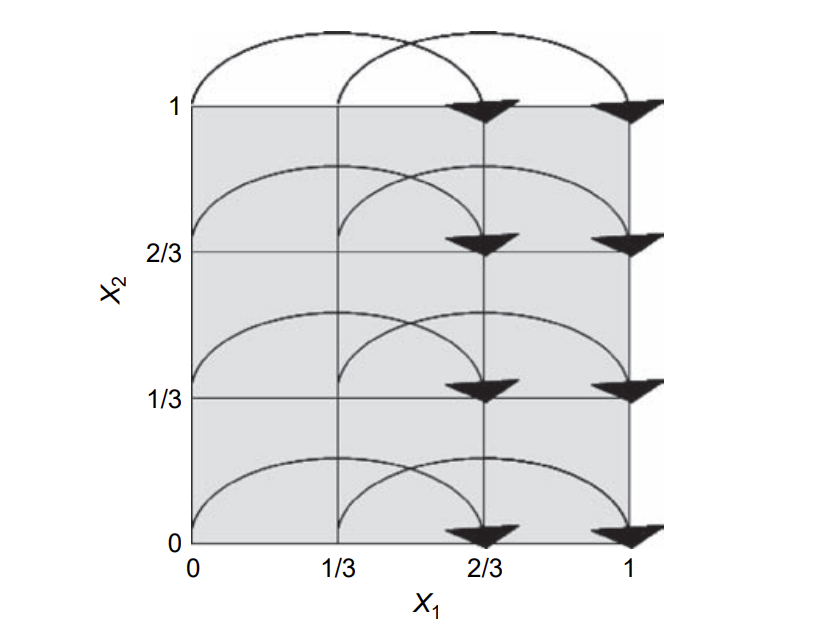
\includegraphics[width=0.7\textwidth]{Bilder/morris_grid.png}
	\caption{An example grid $\Omega$. The grid features two parameters $X_1$, $X_2$, meaning that it is a two-dimensional grid. Further, it features four levels ($p = 4$). The step length $\Delta$ chosen here is $\frac{2}{3}$, which corresponds to an element of the set of viable values for $\Delta$: $1 - \frac{1}{4-1} = 1 - \frac{1}{3} = \frac{2}{3}$.}
	\label{fig:morris_grid}
\end{figure}

In the definition of the elementary effect, the vector $\mathbf{X} = (X_1, X_2, \dots, X_k)$ has to fulfil the condition that $\mathbf{X} + \mathbf{e}_i \cdot \Delta$ still has to lie within the grid $\Omega$. $\mathbf{e}_i$ is a vector of zeros except having a one at its $i$th entry. So for instance:

\begin{equation}
	\mathbf{e}_2 = (0, 1, 0, \dots, 0)
\end{equation}

The Morris method occupies itself with finding the statistical distribution of each of the $i$ elementary effects. $\mathcal{F}_i$ is thereby used to denote the distribution of $EE_i$, in other words $\mathcal{F}_i \sim EE_i$ \citep{saltelli_global_2007}.

\subsubsection{Trajectory-Based Sampling}

To populate $\mathcal{F}_i$ with multiple samples of $EE_i$, the Morris method uses an efficient trajectory-based sampling design that obtains as many elementary effects as possible from as few model evaluations as possible.

The exact mathematical formulation of how trajectories are constructed is beyond the scope of this thesis; a visual understanding is sufficient. Figure~\ref{fig:saltelli_trajectory_grid}, taken from \citep{saltelli_global_2007}, shows an example trajectory through a three-dimensional sampling grid.

\begin{figure}[H]
	\centering
	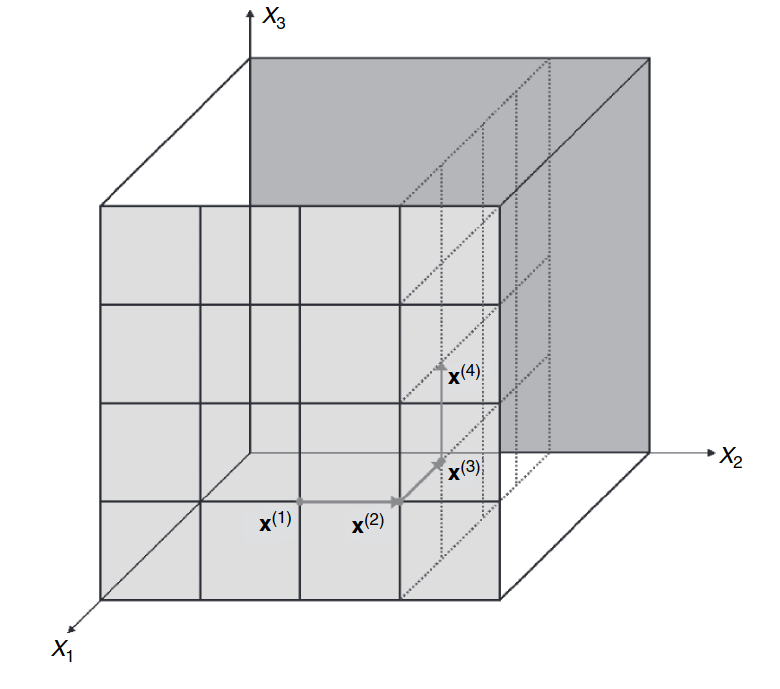
\includegraphics[width=0.7\textwidth]{Bilder/satteli_trajectory_grid.png}
	\caption{An example Morris trajectory through a three-dimensional sampling grid ($k = 3$, $p = 6$). The trajectory consists of $k+1 = 4$ points, with each consecutive pair of points differing in exactly one parameter. Reproduced from \citet{saltelli_global_2007}.}
	\label{fig:saltelli_trajectory_grid}
\end{figure}

From this figure it becomes visible that a trajectory consists of $k+1$ points $\mathbf{x}^{(1)}, \mathbf{x}^{(2)}, \dots, \mathbf{x}^{(k+1)}$, where $k$ is the dimension of the sampling grid. Each point differs from its predecessor by a step of $\Delta$ in exactly one grid direction, so that consecutive points differ in only one parameter. The trajectory is constructed such that each dimension of the grid is stepped along exactly once. Note that since the grid shown is three-dimensional ($k = 3$, matching the three parameters varied in this work), each trajectory consists of $k+1 = 4$ points.



Each trajectory yields exactly k elementary effects $EE_i$, one for each parameter spanning the sampling grid. A single trajectorybrequires $k+1$ model evaluations -- one at each point -- and yields exactly $k$ elementary effects: one estimate for each factor.

To build up $\mathcal{F}_i$ for every factor, $r$ such trajectories are generated. Since each trajectory contributes exactly one elementary effect per factor, each $\mathcal{F}_i$ ends up containing $r$ samples. The total number of model evaluations required is:




\begin{equation}
	N = r \cdot (k+1)
	\label{eq:morris_runs}
\end{equation}


\citep{saltelli_global_2007}.

\subsubsection{Choosing $\Delta$ and $r$}

% TODO: add the r choice

The choice of $p$ and $\Delta$ are not independent. When $p$ is chosen to be even, the choice $\Delta = \frac{p/2}{p-1}$ has the additional property of guaranteeing equal-probability sampling from the grid, meaning that all grid levels are sampled with equal probability across the $r$ trajectories \citep{saltelli_global_2007}.

\subsubsection{Sensitivity Measures: $\mu$, $\sigma$, and $\mu^*$}

Once the distributions $\mathcal{F}_i$ have been mapped out, statistical measures can be computed just like over every other statistical distribution. In Morris, the mean $\mu_i$ and the standard deviation $\sigma_i$ of $\mathcal{F}_i$ are computed. These two statistical measures together already allow for reasonable insight into the influence of the $i$th parameter $X_i$ which corresponds to the $i$th elementary effect $EE_i$:

If $\mu_i$ deviates strongly from $0$, then this means that the elementary effect $EE_i$ generally takes on non-zero values and therefore that the model output changes notably when a step of $\Delta$ is performed along the dimension spanned by $X_i$. This then ultimately means, that changes in $X_i$ seem to generally affect the model output $Y$ considerably and $X_i$ therefore receives a high sensitivity score. Generally, the more $\mu_i$ deviates from zero, the larger the sensitivity of the model output towards $X_i$.

If $\sigma_i$ is large, this means that the distribution $\mathcal{F}_i$ is spread out considerably over a larger range. This indicates, that the elementary effects $EE_i$ that were computed were generally different depending on their location in the grid. Meaning that in one area, the model might only yield small changes in output, when $X_i$ is varied while in other areas $X_i$ leads to strong changes in model output. This behaviour points either to nonlinearity regarding $X_i$ or to the fact that $X_i$ interacts with other input parameters. Which effect is responsible for the high standard deviation (or whether both are responsible for the effect at the same time) can not be determined. Which is a shortcoming of the method of Morris \citep{saltelli_global_2007}. Figure \ref{fig:mu_sig_example} provides an visual example of possible F distributions of a Factor $X_i$ with the associated $\mu$ and $\sigma$ values and the corresponding interpretation.

\begin{figure}[H]
	\centering
	
\includegraphics[width=1\textwidth]{Bilder/example_grid_mu_sigma_vairation.png}
	\caption{Different F distributions of a parameter $X_i$ are shown. Additionally, $\mu$ and $\sigma$ of each distribution is provided. An interpetation is provided}
	\label{fig:mu_sig_example}
\end{figure}

Situations can occur, where $\mathcal{F}_i$ contains many extreme values however the distribution is symmetric around zero. One such example is visualized in \ref{fig:mu_sig_example} in the upper left plot. In such cases computing the mean value $\mu_i$ will yield a value close to zero and we would assume, that the parameter $X_i$ therefore is noninfluential. This would be a faulty assumption, as the sampled elementary effects $EE_i$ are substantial in their magnitude but just cancel themselves out. This phenomenon can be spotted by always taking $\sigma_i$ into consideration, as in this scenario $\sigma_i$ is large, but it is more common to also sample an additional distribution $\mathcal{G}_i$ which captures the magnitude of the elementary effects $|EE_i|$. So $\mathcal{G}_i \sim |EE_i|$. We then compute the mean of this distribution $\mu^*_i$ which can be interpreted like $\mu_i$. The further away from zero, the more influential is the parameter. But since it is the magnitude, the distribution never features negative values and therefore cancellation effects can not occur \citep{saltelli_global_2007}. Figure \ref{fig:mu_mu_star} provides a visual example for this phenomenon.

\begin{figure}[H]
	\centering
	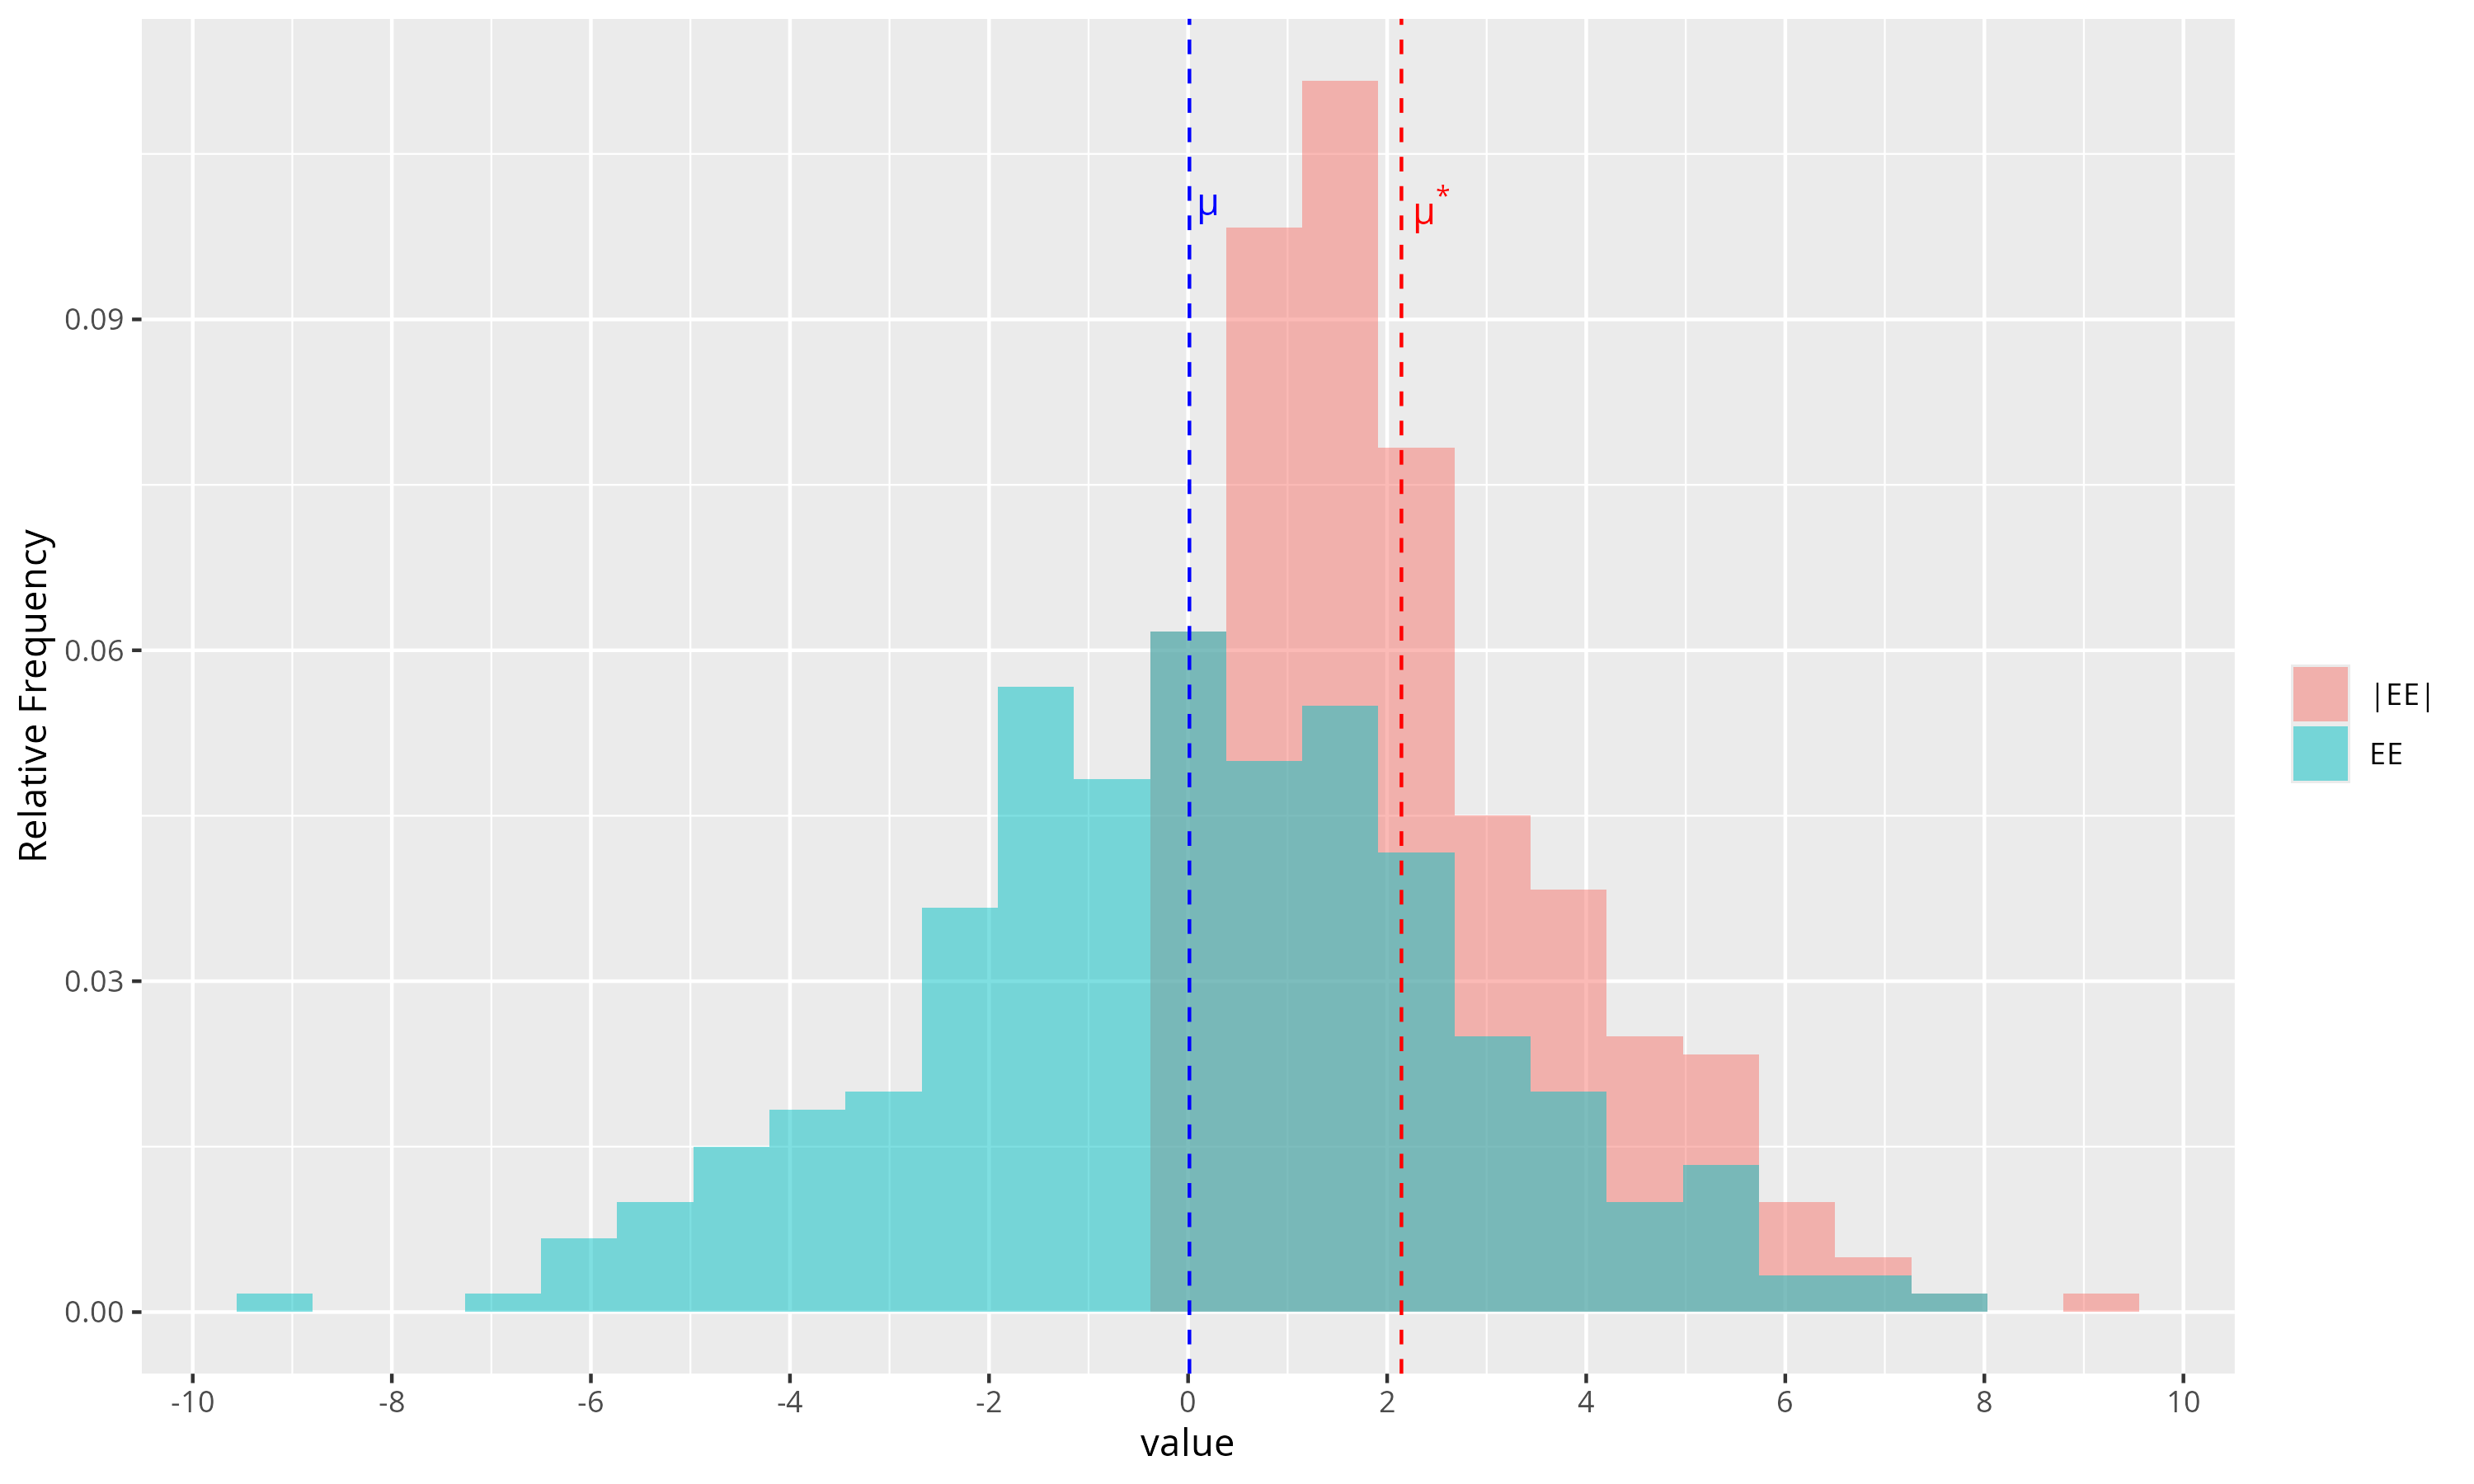
\includegraphics[width=1\textwidth]{Bilder/mu_mu_star.png}
	\caption{The difference of $\mu$ and c visualized with their underlying distribution $\mathcal{G}$ and $\mathcal{F}$. While the mean $\mu$ of the distributuion $\mathcal{F}$ lies at around zero, $\mu^{\star}$ significantly deviates from zero}
	\label{fig:mu_mu_star}
\end{figure}

% Here a range of example parameter plots are needed to show how FF_i distributions can look like, how they can be skewed, how they can be symetric etc.


\section{Coldwater Patches}

Cold water patches (CWPs) are areas in rivers and streams where the water temperature is measurably colder than that of the main channel. The temperature difference used to define a CWP varies across the literature but is typically set between 0.5 and 3 degrees Celsius below the main channel temperature \citep{casas-mulet_unmanned_2020, wawrzyniak_effects_2016}. Cold water patches are not automatically cold water refugia. Cold water refugia are cold water patches that are actively used by cold-water organisms for thermal relief \citep{mejia_closing_2023}. The ecological importance of cold water refugia is expected to increase as river temperatures rise due to climate change \citep{kurylyk_preserving_2015}.

%% Missing %%

% TODO: hot to choose r and how choosing r and k determines how many runs
% TODO: that these things are generally most of the time for 1D models, and that we derefore have to get createive


	\chapter{Methods}

This chapter describes the operationalisation of the three research questions 
into a set of methodological steps, which are then described in detail. The 
first section addresses research question 1 by describing the reimplementation 
of the CWP detection algorithm and the comparison of its outputs and runtime 
against the original. The second section addresses research question 2 by 
describing the Morris sensitivity analysis, including the selection and 
classification of CWPs, the computation of sensitivity indices, and the 
subsequent visualisation and statistical modelling. The third section addresses 
research question 3 by describing the algorithm modifications derived from the 
sensitivity analysis findings. A description of the data and study area is 
provided first.

\chapter{Methods}

This chapter describes the operationalisation of the three research questions 
into a set of methodological steps, which are then described in detail. The 
first section addresses research question 1 by describing the reimplementation 
of the CWP detection algorithm and the comparison of its outputs and runtime 
against the original. The second section addresses research question 2 by 
describing the Morris sensitivity analysis, including the selection and 
classification of CWPs, the computation of sensitivity indices, and the 
subsequent visualisation and statistical modelling. The third section addresses 
research question 3 by describing the algorithm modifications derived from the 
sensitivity analysis findings. A description of the data and study area is 
provided first.

\section{Data and Study Area}

The Emme river originates in an extensive moorland between the Hohgant and 
Augstmatthorn massifs and flows through the Emmental region before joining 
the Aare near Zuchwil/Luterbach. The catchment covers approximately 
974~km$^2$ with a mean elevation of 845~m~a.s.l., and land cover is 
dominated by agricultural land (52.1\%) and forested areas (37.9\%). 
During summer thunderstorms, the river can rise rapidly within minutes 
and transport large quantities of driftwood; as a consequence, the lower 
reaches have been heavily engineered \citep{tonolla_thermische-kartographie_2026}.

\citet{tonolla_thermische-kartographie_2026} acquired high-resolution TIR 
and RGB orthophotos along a 69~km transect of the Emme main channel, 
spanning from Kemmeribodenbad~BE to Biberist~SO, as well as imagery of 
three tributary rivers: the Ilfis, Grüene, and Urtene. The TIR imagery was 
collected from a helicopter platform using a FLIR SC655 thermal infrared 
camera. In this thesis, only the TIR and RGB orthophotos of the 69~km 
main channel section are used. The TIR orthophotos serve as the primary 
input to the CWP detection algorithms, while the RGB orthophotos are used 
in a downsampled state as background images for selected visualisations 
and were not used for any further analytical purpose. The 69~km river 
transect is covered by three partially overlapping single-band TIR 
orthophotos. Figure~\ref{fig:study_area} provides an overview of the study 
area, showing the settlements demarcating each segment, the three orthophoto 
extents, and the three imaged tributaries. Table~\ref{tab:tir_specs} 
summarises their technical specifications.

\begin{figure}[H]
	\centering
	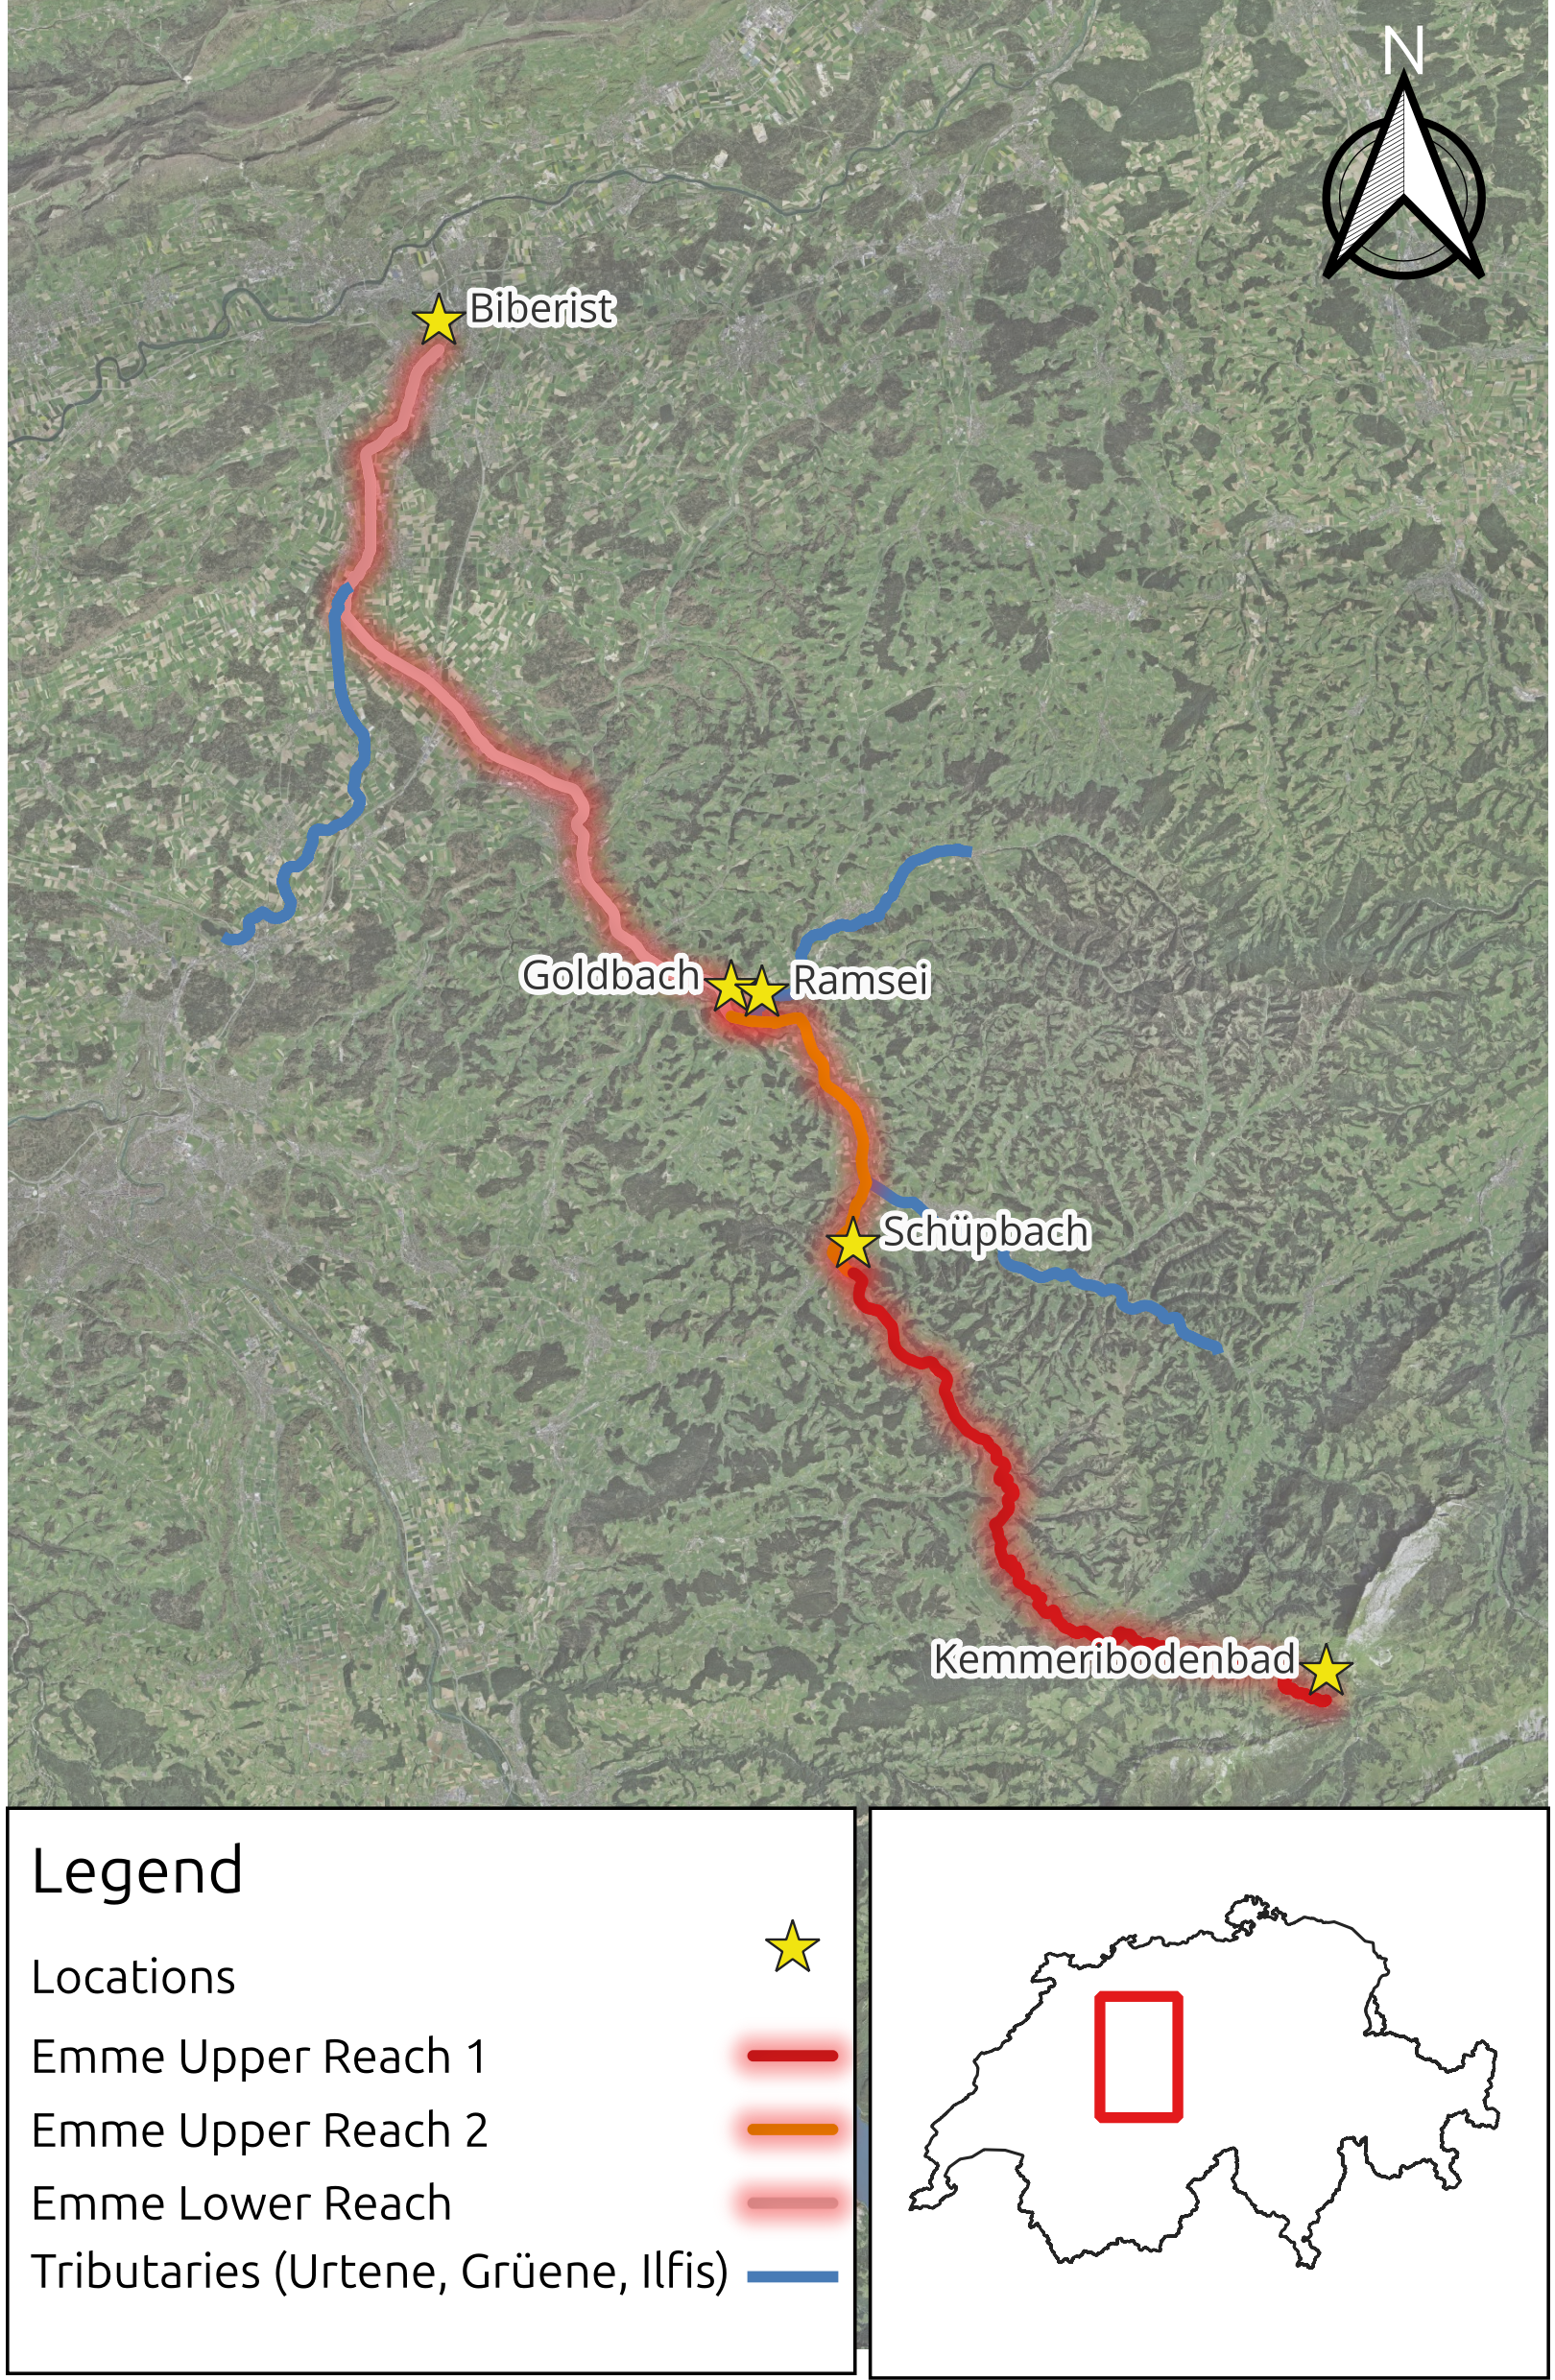
\includegraphics[width=\textwidth]{Bilder/study_area_map.png}
	\caption{Overview of the study area along the Emme river. The map shows 
		the settlements bounding each of the three TIR orthophoto segments 
		(Emme Upper Reach 1, Emme Upper Reach 2, Emme Lower Reach), as well as 
		the three tributary rivers imaged during the survey (Ilfis, Grüene, 
		and Urtene), shown here as a single combined category.}
	\label{fig:study_area}
\end{figure}

\begin{table}[H]
	\centering
	\caption{Technical specifications of the three TIR orthophotos covering 
		the Emme main channel. All rasters are in the Swiss coordinate reference 
		system CH1903+/LV95 (EPSG:2056) and stored as single-band Float32 
		GeoTIFF files.}
	\label{tab:tir_specs}
	\begin{tabular}{@{} l p{3.5cm} p{3.5cm} p{3.5cm} @{}}
		\toprule
		& \textbf{Emme Upper Reach 1} 
		& \textbf{Emme Upper Reach 2} 
		& \textbf{Emme Lower Reach} \\
		\midrule
		Extent
		& Kemmeribodenbad -- Schüpbach
		& Schüpbach -- Goldbach
		& Ramsei -- Biberist \\
		\addlinespace
		Total pixels   
		& $4.75 \times 10^9$ 
		& $8.45 \times 10^8$ 
		& $6.57 \times 10^9$ \\
		Resolution (m)    
		& $0.207 \times 0.207$ 
		& $0.204 \times 0.204$ 
		& $0.207 \times 0.207$ \\
		Min temp.\ (\textdegree C) & 7.43  & 10.08 & 12.50 \\
		Max temp.\ (\textdegree C) & 33.67 & 30.94 & 34.10 \\
		Mean temp.\ (\textdegree C) & 20.85 & 18.84 & 20.90 \\
		Std dev.\ (\textdegree C)  &  1.05 &  1.24 &  1.32 \\
		\bottomrule
	\end{tabular}
\end{table}

\section{Addressing Research Question 1: Algorithm Reimplementation}
\label{sec:rq1_methods}

Performing the Morris sensitivity analysis requires $r \times (k+1)$ model 
evaluations (Equation~\ref{eq:morris_runs}); for $k=3$ parameters and $r=64$ 
trajectories this amounts to 256 executions. Given that the existing CWP 
algorithm requires between 1.25 and 2 hours per run, parallel execution on 
ZHAW's High Performance Cluster (HPC) is necessary to complete the experiment 
within a feasible timespan. To ensure that optimisation gains carry over to 
the HPC infrastructure, all benchmarking was performed directly on the cluster. 
In the remainder of this thesis, the original implementation is referred to as 
v1 and the speed-optimized reimplementation as v2.

\subsection{Reimplementation of the CWP Algorithm based on GDAL and System Calls}

The reworked algorithm preserves the computational logic of the original 
implementation but differs fundamentally in how each step is mechanistically 
executed. Where the original algorithm processes the raster slab-by-slab in 
memory using R loops and \texttt{terra}/\texttt{sf} functions, the reworked 
algorithm replaces these with calls to the GDAL command line interface, operating 
directly on raster and vector files on disk rather than holding intermediate 
results in memory. Table~\ref{tab:cwp_pseudocode} gives a high-level overview of 
the reimplemented algorithm; the tool or function used in each step is listed in 
the right-hand column. The remainder of this section motivates the key design 
decisions underlying this choice of implementation.

\begin{table}[H]
	\centering
	\caption{High-level overview of the reworked CWP detection algorithm, 
		including the primary tool or function used for each step.}
	\label{tab:cwp_pseudocode}
	\begin{tabular}{@{}c p{7.5cm} p{4cm}@{}}
		\toprule
		\textbf{Step} & \textbf{Description} & \textbf{Tool / Function} \\
		\midrule
		1 & Divide the river reach into $n$ centerline segments; construct a 
		wide zone polygon and a narrow reference-strip polygon for each 
		segment. & \texttt{sf::st\_buffer} \\
		\addlinespace
		2 & Rasterize the zone polygons to a raster matching the TIR raster 
		resolution, using the segment id as burn-in value. & 
		\texttt{gdal vector rasterize} \\
		\addlinespace
		3 & Round the TIR raster using a fixed rounding factor. & 
		\texttt{gdal raster calc} \\
		\addlinespace
		4 & Extract the median temperature per segment from the rounded TIR 
		raster within each reference strip; store in a look-up table keyed 
		by segment id. & \texttt{exactextractr::exact\_extract} \\
		\addlinespace
		5 & Reclassify the zone raster, replacing each segment id with its 
		reference temperature from the look-up table, yielding the reference 
		raster. & \texttt{gdal raster reclassify} \\
		\addlinespace
		6 & Subtract the rounded TIR raster from the reference raster; flag 
		pixels where the difference exceeds $\Delta T$, producing a binary 
		CWP raster. & \texttt{gdal raster calc} \\
		\addlinespace
		7 & Polygonize the binary CWP raster into patch polygons. & 
		\texttt{terra::as.polygons} \\
		\addlinespace
		8 & Filter patches by minimum area, compute per-patch temperature 
		statistics, and apply a patch-level threshold check against the 
		reference temperature. & \texttt{exactextractr::exact\_extract} \\
		\bottomrule
	\end{tabular}
\end{table}

\paragraph{Performance.} The decision to heavily rely on GDAL was made as 
\texttt{terra} operations are sometimes not performant, and GDAL offers an often 
faster set of geocomputational tools, which can be called from R using 
\texttt{system()} or \texttt{sf::gdal\_utils()} \citep{lovelace2019geocomputation}. 
Empirical testing in a prior coursework exercise also showed a significant speedup 
of GDAL-based raster operations compared to \texttt{terra} across a range of use 
cases \citep{duerr_raster_deepdive}; this coursework was not peer-reviewed and is 
cited here only as a supporting empirical observation.

\paragraph{Memory footprint and HPC suitability.} Operating directly on disk 
rather than in memory keeps the memory footprint small, which is important in 
an HPC setting where available memory can become a limiting factor under 
parallel execution. The drawback is that intermediate rasters can reach up to 
25\,GB in size; this was addressed by applying \texttt{COMPRESS=DEFLATE} with 
\texttt{PREDICTOR=2} when writing GeoTIFF files \citep{gdal_gtiff_driver}, 
which substantially reduces disk space consumption with negligible computational 
overhead.

\paragraph{Raster value extraction.} \texttt{terra::extract()} was replaced 
with \texttt{exact\_extract()} from the \texttt{exactextractr} package (steps 
4 and 8 of Table~\ref{tab:cwp_pseudocode}), which extracts aggregated raster 
values considerably faster for large rasters \citep{mieno_rgis_2022}. The two 
functions differ in how partially covered cells are handled: 
\texttt{exact\_extract()} weights cells by their coverage fraction 
\citep{isciences_exactextract}, whereas \texttt{terra::extract()} includes a 
cell only if its centre point falls within the polygon 
\citep{hijmans_terra_extract} -- the behaviour used in v1. To approximate this, 
only cells with a coverage fraction of at least 50\% were included in 
\texttt{exact\_extract()}; this approximation is not exactly equivalent to 
\texttt{terra}'s centre-point rule.

\subsection{Output Equivalence and Runtime Comparison}
\label{sec:output_equivalence}

The resulting reimplementation was tested for equivalence in output by comparing 
the CWP polygons produced by v2 against those produced by v1 when deployed with 
the exact same set of parameters. Spatial agreement was assessed using the 
Jaccard similarity index:

\begin{equation}
	J(A, B) = \frac{\text{area}(A \cap B)}{\text{area}(A \cup B)}
	\label{eq:jaccard}
\end{equation}

where $A$ and $B$ are the CWP polygon sets produced by v1 and v2 respectively. 
$J = 1$ indicates perfect agreement and $J = 0$ indicates no overlap. In 
addition, visual inspection in QGIS was carried out to identify any systematic 
spatial patterns in the disagreements. Table~\ref{tab:validation_params} shows 
the parameter combinations used in testing.

Runtime was compared across three segment lengths (400, 800, and 1200~m), with 
all other parameters held constant (zone halfwidth = 60~m, buffer = 3~px, 
$\Delta T = 1.0\,^{\circ}$C, minimum patch area = 2~m$^2$, rounding = 
$0.1\,^{\circ}$C, 8-connectivity enabled).

\begin{table}[H]
	\centering
	\caption{Parameter combinations used for the output equivalence comparison 
		between v1 and v2.}
	\label{tab:validation_params}
	\begin{tabular}{@{}l c c c@{}}
		\toprule
		\textbf{Parameter} & \textbf{Test 1} & \textbf{Test 2} & \textbf{Test 3} \\
		\midrule
		\texttt{segment\_length\_m}   & 200  & 800  & 1200 \\
		\texttt{zone\_halfwidth\_m}   & 60   & 60   & 60   \\
		\texttt{buffer\_px}           & 4    & 3    & 5    \\
		\texttt{delta\_C}             & 0.5  & 1.0  & 1.5  \\
		\texttt{min\_patch\_area\_m2} & 2    & 3    & 2    \\
		\texttt{round\_to}            & 0.1  & 0.1  & 0.1  \\
		\texttt{connect\_diagonals}   & TRUE & TRUE & TRUE \\
		\bottomrule
	\end{tabular}
\end{table}


\section{Addressing Research Question 2: Sensitivity Analysis}
\label{sec:rq2_methods}

With the algorithm optimized, sensitivity analysis can now be carried out to 
determine the sensitivity of the CWP detection algorithm with respect to the 
parameters buffer pixel count, step length, and temperature delta. The first 
step focuses on determining CWPs that are susceptible to the step length 
parameter and classifying them into tributary-caused and non-tributary-caused 
CWPs. The second step derives Morris sensitivity indices for these CWPs with 
respect to their area. The third step displays the results visually and fits 
a statistical model relating step-length sensitivity to CWP area and temperature 
delta.

The inclusion of buffer pixel count and temperature delta alongside step length 
also serves a secondary, validatory purpose. \citet{tonolla_thermische-kartographie_2026} 
found that the buffer pixel count has little influence on CWP area, while the 
temperature delta parameter was among the most influential. Replicating both 
findings within the present methodology would lend additional credibility to 
both approaches.

\subsection{Determining and Classifying Step Length Sensitive CWP}
\label{sec:cwp_classification}

Especially of interest is to observe the difference in sensitivity towards the 
step length parameter between tributary-caused and non-tributary-caused CWP. For 
this reason, a pre-selection method is deployed to guarantee that the studied CWP 
are sensitive towards the step length parameter. A Morris design with $r=44$ and 
$k=2$ is first set up for the buffer pixel count and step length parameters. Then 
the speed-optimized (v2) CWP algorithm is deployed on the resulting parameter 
tuples. Lastly, the results are aggregated to a fuzzy representation of the CWP 
over all runs, to then select CWP which are variable with respect to the CWP 
algorithm and to classify them into tributary-caused and non-tributary-caused CWP. 
Figure~\ref{fig:cwp_fuzzy_overview} provides a visual overview of these steps.

\begin{figure}[H]
	\centering
	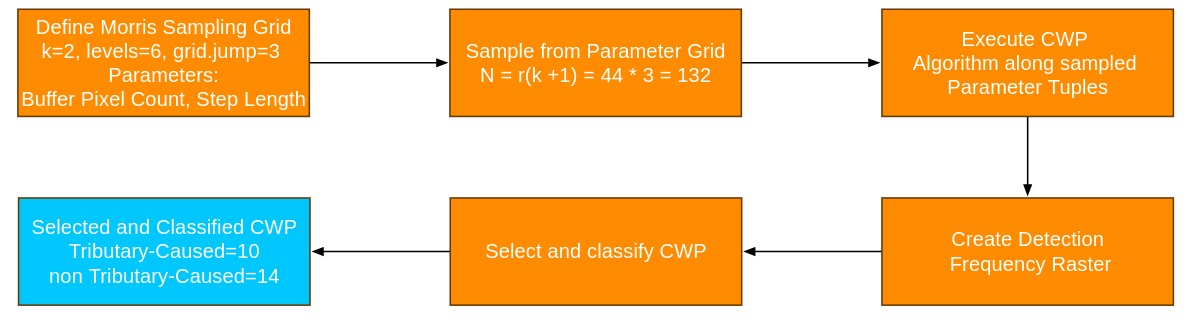
\includegraphics[width=\textwidth]{Bilder/cwp_fuzzy.png}
	\caption{Visual overview of the steps involved in determining and classifying 
		step-length-sensitive CWP. The result is a set of classified CWPs.}
	\label{fig:cwp_fuzzy_overview}
\end{figure}

\subsubsection{Setting up First Morris Experiment}

A two-dimensional Morris sampling grid was set up spanning buffer pixel count 
and step length, with 6 levels per parameter (step length: 400--1200~m; buffer: 
2--7~px), using the R package \texttt{sensitivity}
to generate the sampling design. In this package, the step size is not set 
directly as a continuous value $\Delta$, but rather through the 
\texttt{grid.jump} argument, an integer specifying the number of grid levels 
to be jumped when computing each elementary effect. A \texttt{grid.jump} of 
$3$ was chosen because it corresponds to the recommended step size 
(see \ref{sec:choosing_delta_r}), which implements equal-probability sampling 
of the elementary effects, given by:
\begin{equation}
	\Delta = \frac{p}{2(p-1)} = \frac{6}{2 \times 5} = \frac{3}{5}
\end{equation}
Since the spacing between adjacent levels of the 6-level grid in the 
normalized unit space is $1/(p-1) = 1/5$, jumping 3 grid levels yields 
exactly $3 \times 1/5 = 3/5$, matching the recommended $\Delta$. 
Figure~\ref{fig:morris_grid} shows the grid with the jump distance drawn in. 
A total of 44 trajectories were sampled ($r = 44$), yielding 
$44 \times (2+1) = 132$ parameter tuples, each holding a unique combination 
of buffer pixel count and step length.

% NOTE: filename collision with the second grid's figure (k=3, isometric cube) --
% this k=2 grid needs its own distinct filename.

\begin{figure}[H]
	\centering
	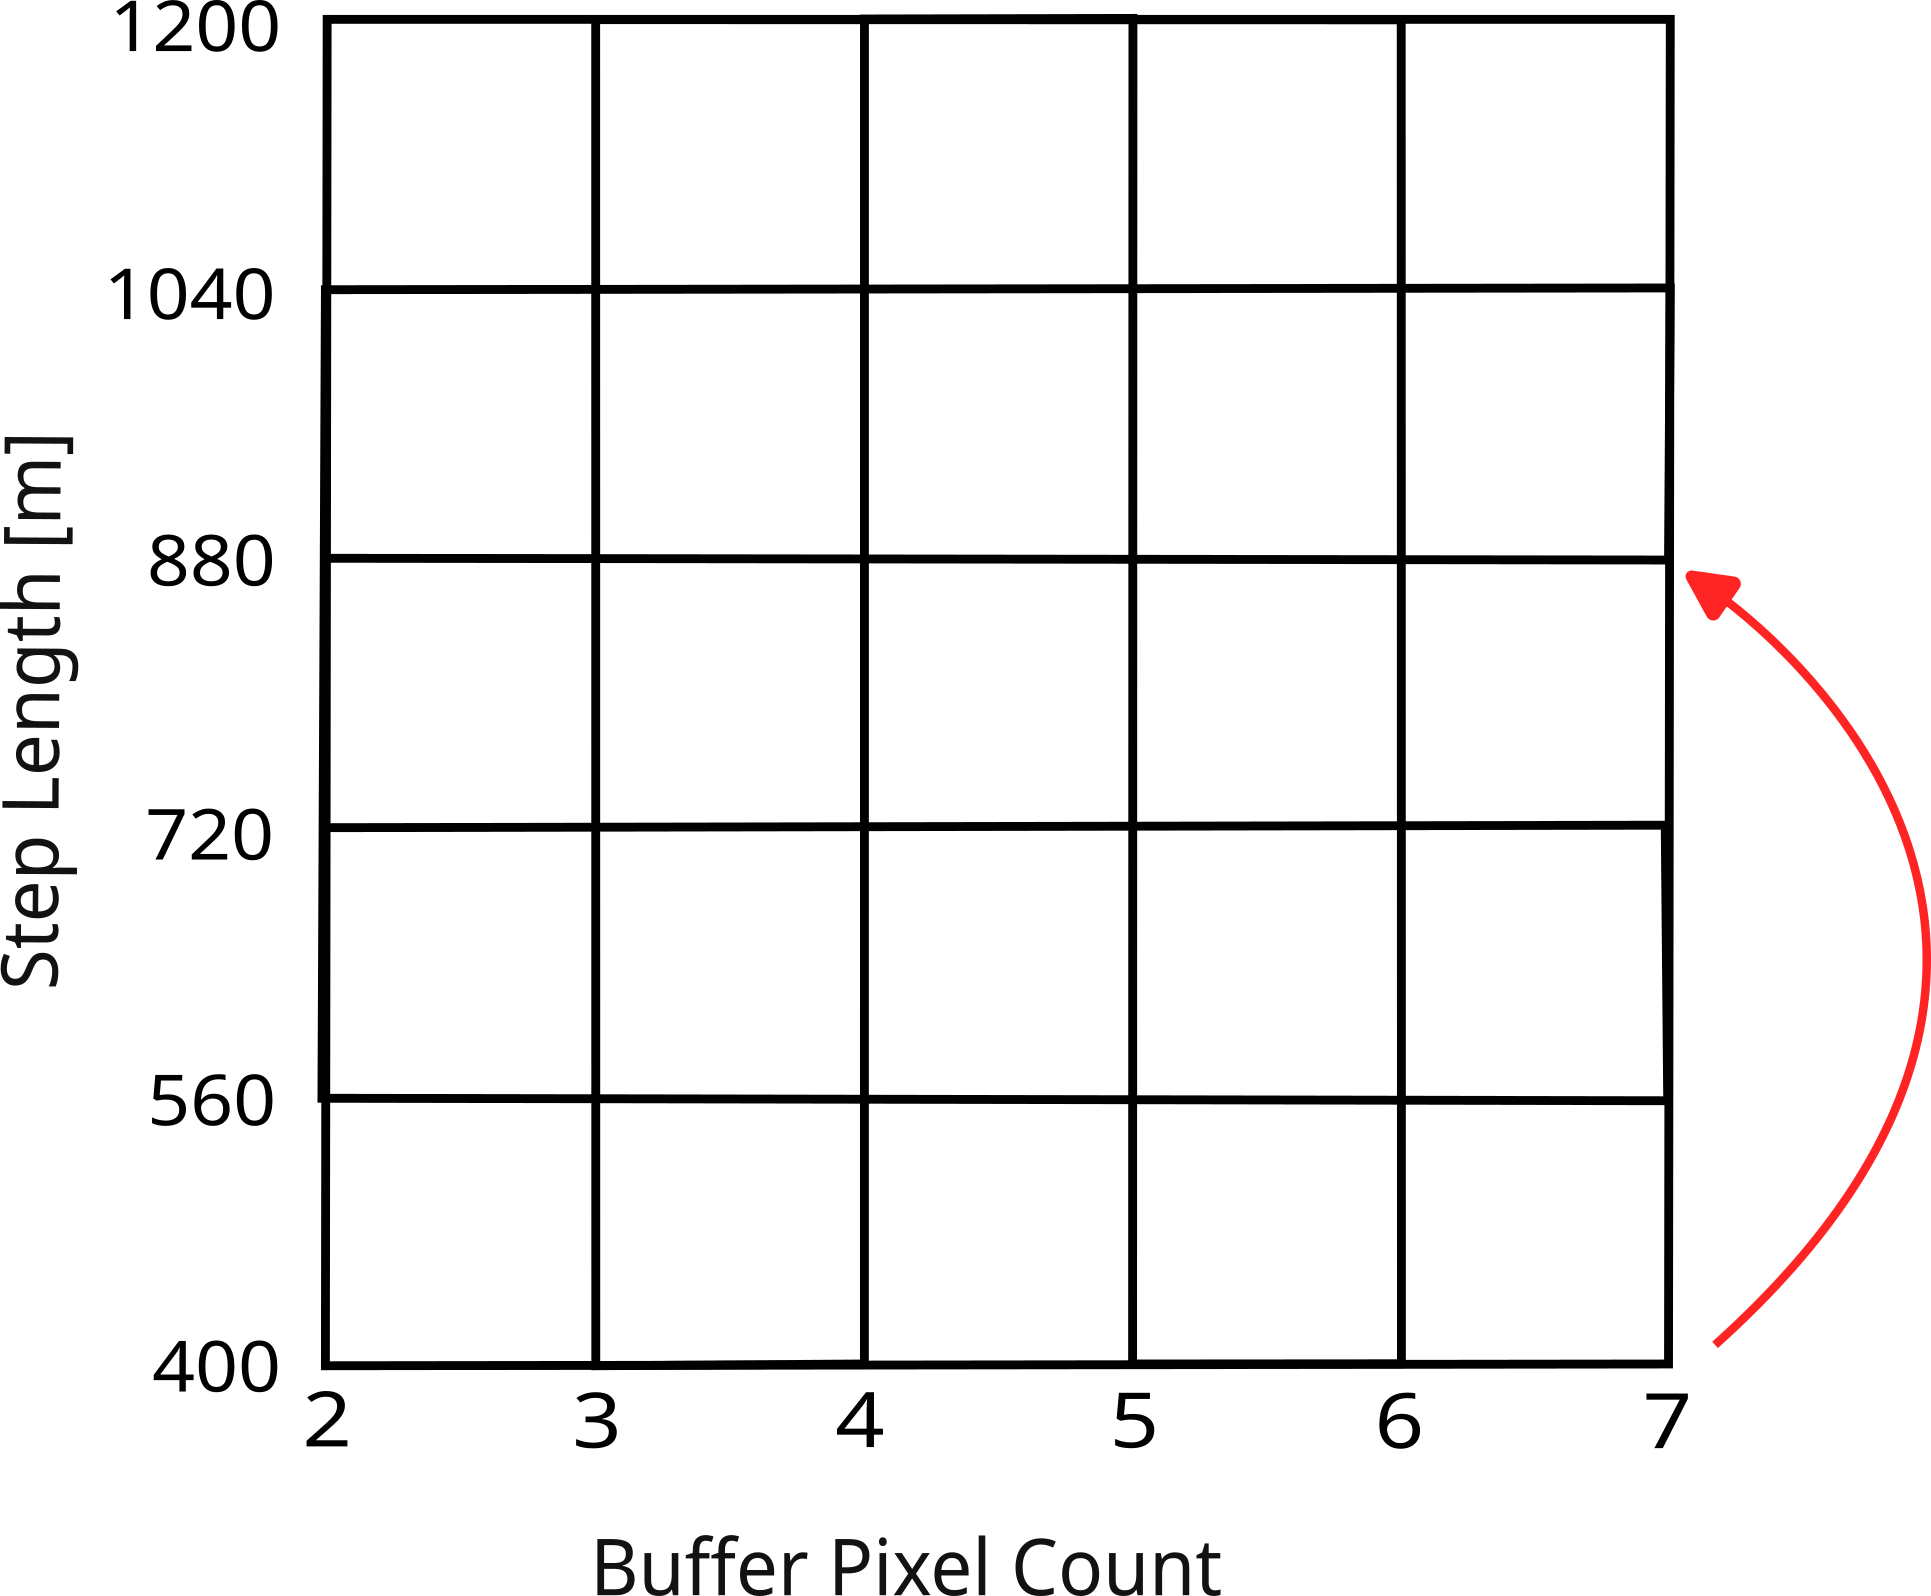
\includegraphics[width=0.8\textwidth]{Bilder/morris_grid_image.png}
	\caption{Visual depiction of the Morris sampling grid, spanning step length 
		and buffer pixel count. The arrow shows the $\Delta$ chosen for the Morris 
		experiment, corresponding to a jump of 3 grid cells.}
	\label{fig:morris_grid}
\end{figure}

The temperature delta parameter was held constant ($k=2$) because varying it 
would introduce variability in the detected extent of essentially all CWPs -- 
making it impossible to distinguish CWPs that are sensitive to step length from 
those that merely respond to a changing detection threshold. Holding it constant 
ensures that any variability in the fuzzy overlay can be attributed to step 
length and buffer pixel count, and in particular to step length, as the buffer 
pixel count is generally non-influential. Further, a Morris design was used 
rather than a simple grid sweep to ensure construct validity of the selection 
criterion: any variability visible in the fuzzy overlay is, by construction, of 
the kind that the subsequent Morris sensitivity analysis is designed to detect. 
Had a different sampling scheme been used, visually variable CWPs might not 
register as sensitive under the Morris indices computed in the second experiment.

\subsubsection{Model Evaluation along Parameter Combinations}
\label{sec:modeleval}

The CWP algorithm was evaluated across all sampled parameter tuples in parallel 
using GNU Parallel \citep{tange_2024_gnu_parallel}, with the remaining parameters 
held constant as listed in Table~\ref{tab:held_constant_first_morris}. Each 
worker process fetched a parameter tuple, created a uniquely named working 
directory, and wrote all results there for traceability. 
Figure~\ref{fig:gnu} visualizes the workflow.

\begin{table}[H]
	\centering
	\caption{Parameter values held constant during the first Morris experiment, 
		while step length and buffer pixel count were varied.}
	\label{tab:held_constant_first_morris}
	\begin{tabular}{lr}
		\toprule
		Parameter & Value \\
		\midrule
		\texttt{zone\_halfwidth\_m}   & 60 m \\
		\texttt{delta\_C}             & 1.0 $^{\circ}$C \\
		\texttt{min\_patch\_area\_m2} & 2 m$^2$ \\
		\texttt{connect\_diagonals}   & TRUE \\
		\texttt{round\_to}            & 0.1 \\
		\bottomrule
	\end{tabular}
\end{table}

\begin{figure}[H]
	\centering
	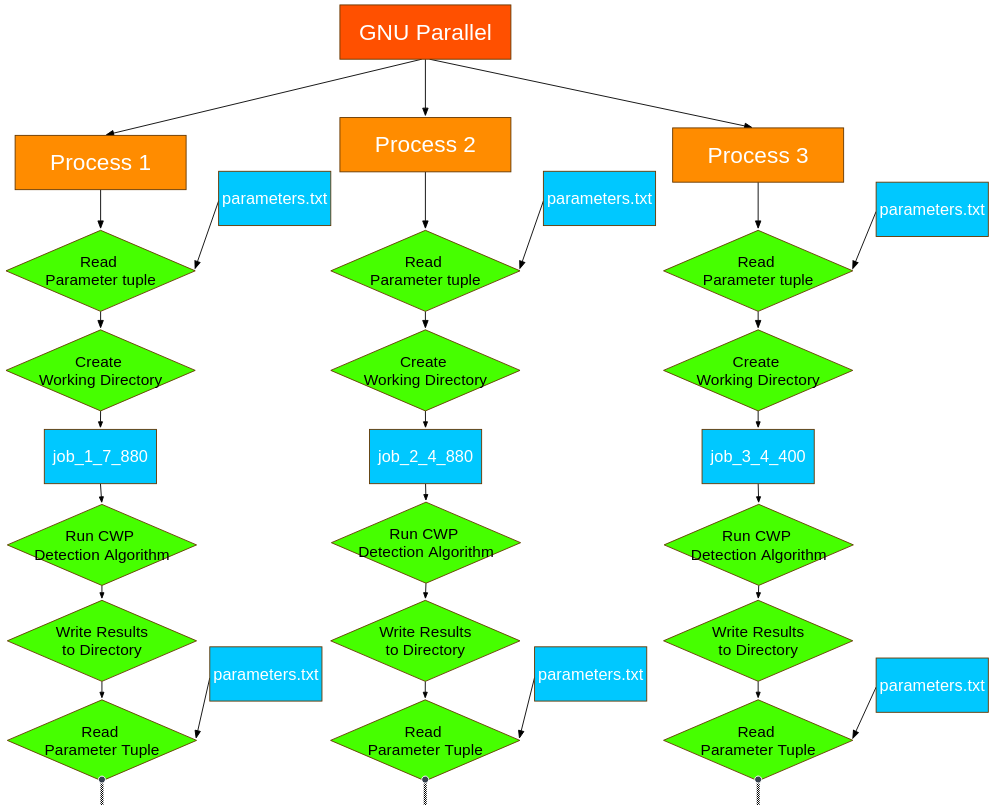
\includegraphics[width=\textwidth]{Bilder/GNU.png}
	\caption{Worker pool orchestrated by GNU Parallel across three parallel 
		processes. Each process reads a parameter tuple from a shared 
		\texttt{parameters.txt} file, creates an individual working directory 
		named after the tuple identifier and parameter values (e.g.\ 
		\texttt{job\_1\_7\_880}), executes the CWP detection algorithm, and 
		writes the results to that directory before fetching the next parameter 
		tuple. The cycle repeats until all tuples have been processed.}
	\label{fig:gnu}
\end{figure}

\subsubsection{Creation of a Fuzzy Overlay of CWP}

The CWP polygon layers from all runs were rasterized at the TIR raster 
resolution, stacked into a multi-layer raster, and reduced to a single 
two-dimensional raster via pixel-wise mean. The result is visualized in 
Figure~\ref{fig:fuzzy_overlay}.

\begin{figure}[H]
	\centering
	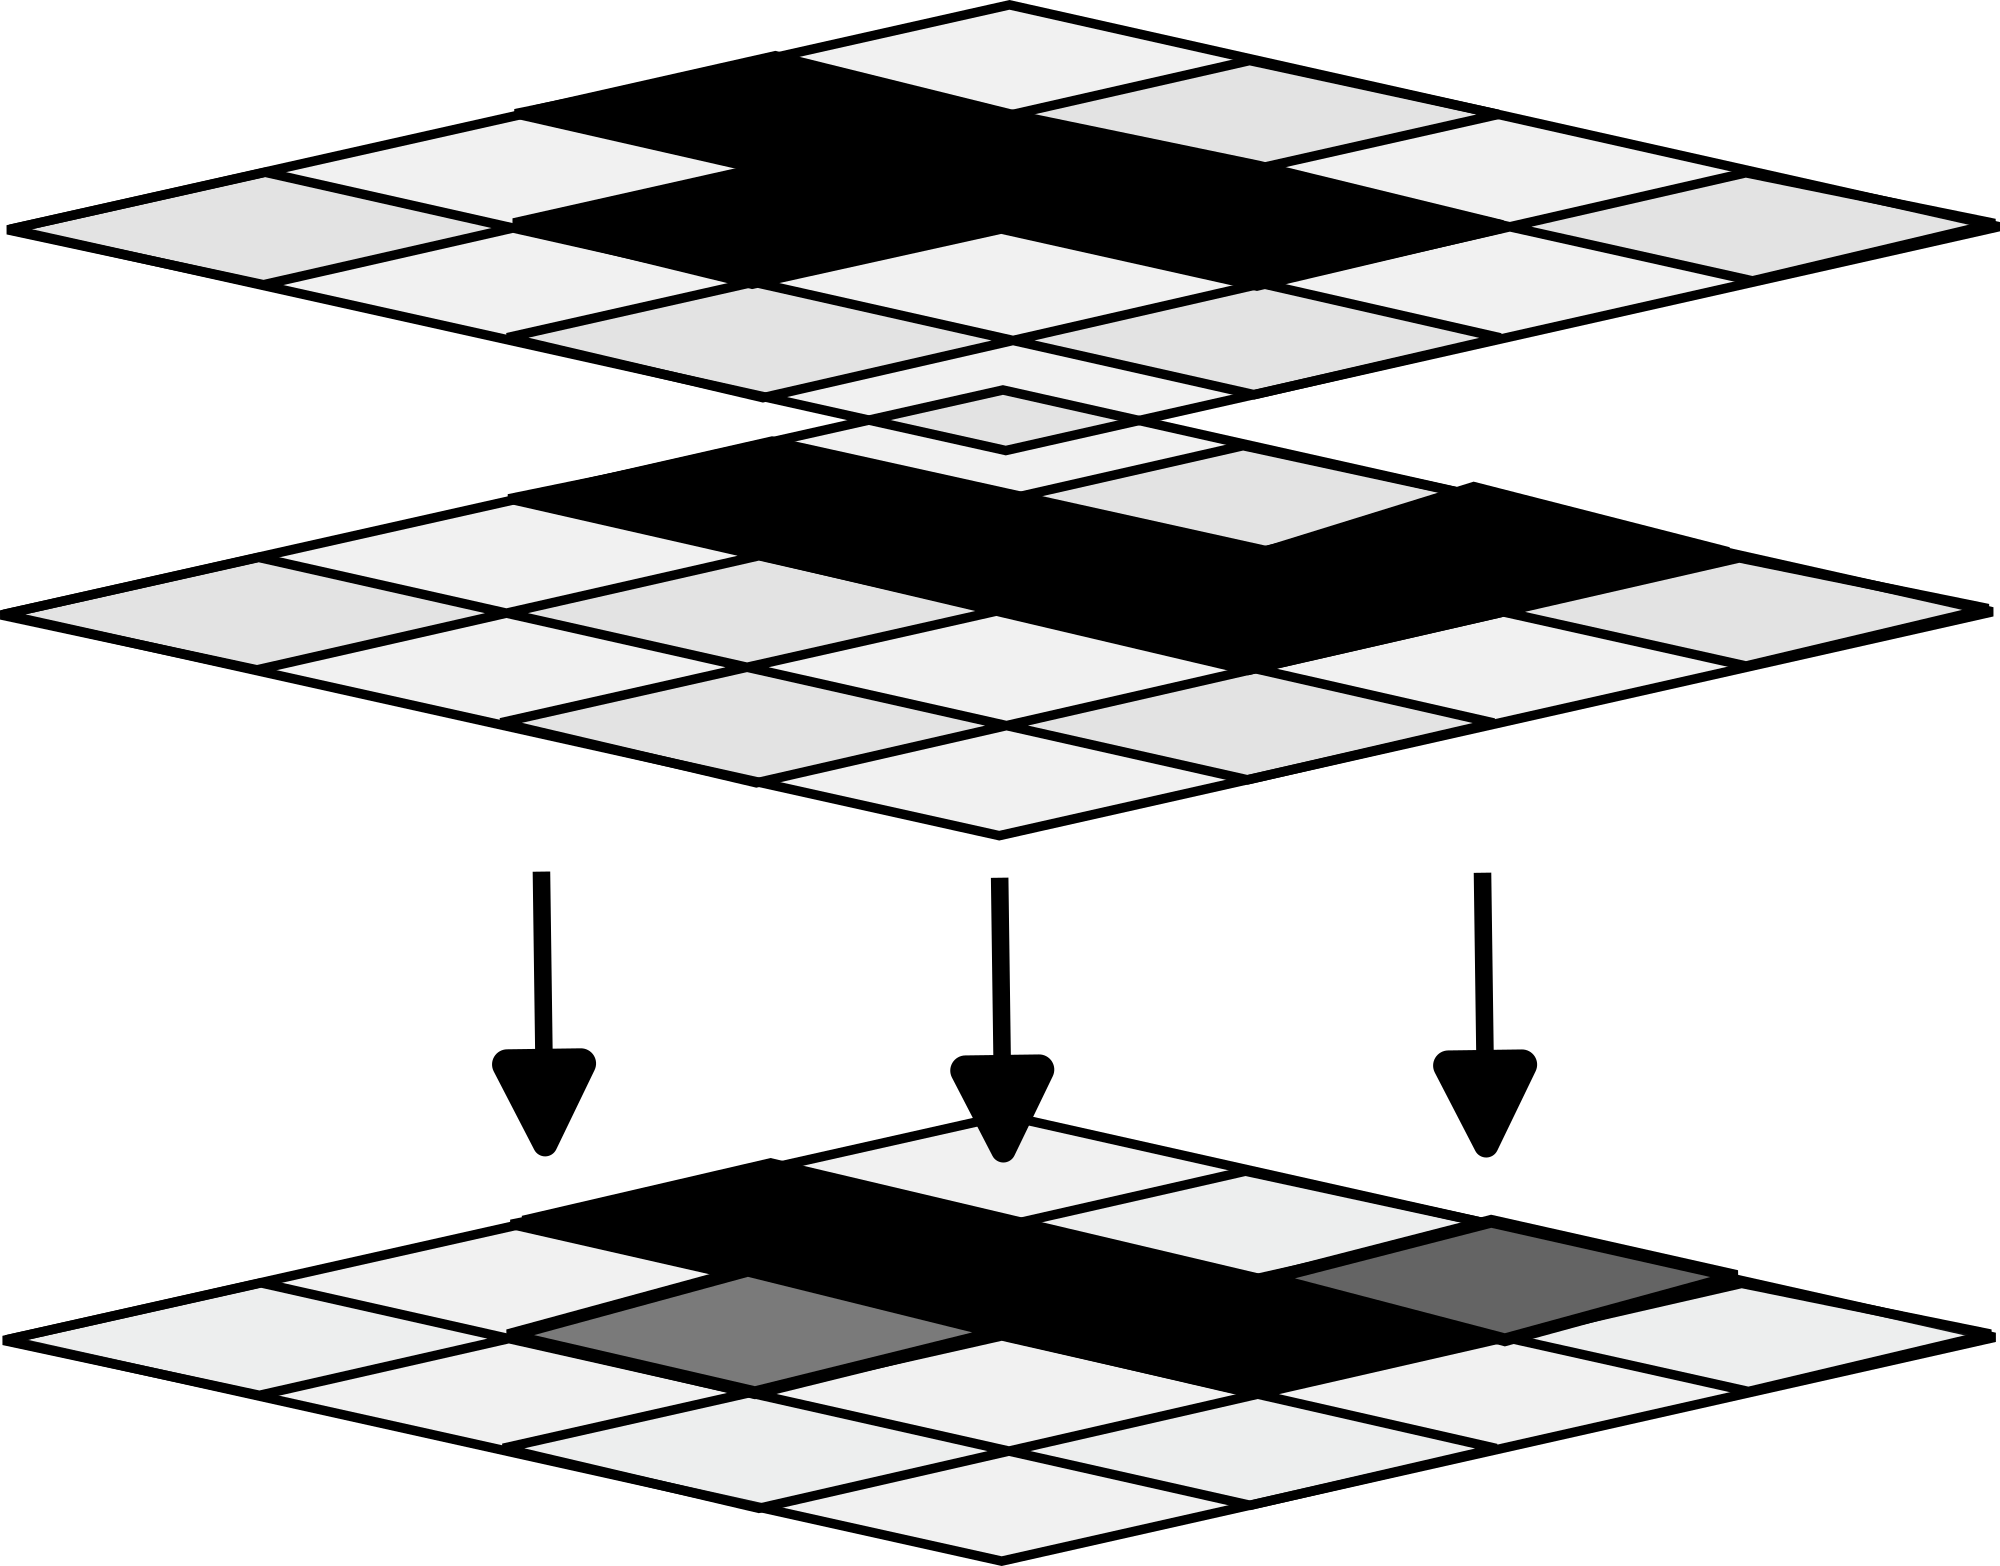
\includegraphics[width=0.8\textwidth]{Bilder/overlay.png}
	\caption{Illustration of the fuzzy overlay construction. The two upper 
		rasters show the binary CWP detection outputs of two individual Morris 
		runs, where dark blue pixels indicate detected CWP and white pixels 
		indicate non-CWP area. The lower raster shows the resulting fuzzy 
		overlay, where light blue pixels hold a lower score than dark blue 
		pixels, reflecting locations where CWP detection was inconsistent 
		across runs.}
	\label{fig:fuzzy_overlay}
\end{figure}

Each pixel in the resulting raster holds a score between 0 and 1, 
representing the fraction of runs in which that pixel was detected as part 
of a CWP -- interpretable as a fuzzy membership score. CWPs showing a wide 
range of scores across their extent are variable with respect to the step 
length parameter and are therefore candidates for the selection and 
classification process described in the following subsection.

\subsubsection{Selection and Classification of CWP}

From the fuzzy CWP raster, patches that were clearly variable and clearly 
attributable to either a tributary inflow or its absence were selected and 
classified as tributary-caused or non-tributary-caused based on visual 
interpretation. Variability was assessed from the fuzzy overlay coloring, 
and tributary attribution was determined by proximity to a tributary inflow. 
Figure~\ref{fig:decision_tree_classification} visualizes this as a decision 
tree.

\begin{figure}[H]
	\centering
	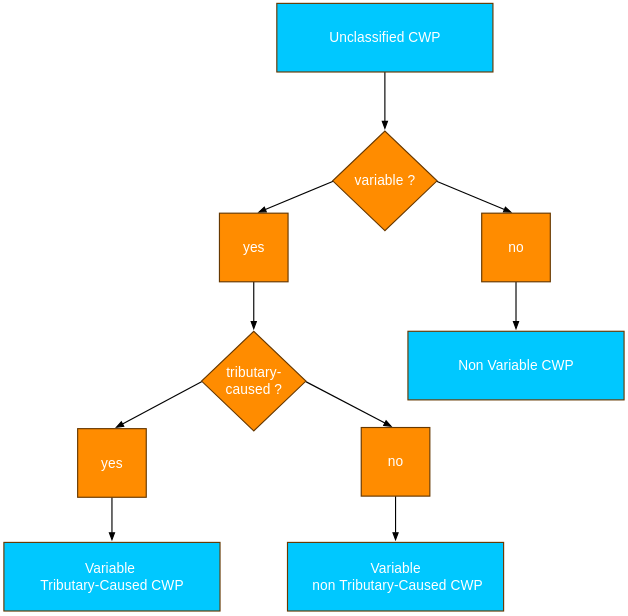
\includegraphics[width=0.8\textwidth]{Bilder/decission_tree_classification.png}
	\caption{Decision tree illustrating the visual classification process applied 
		to candidate CWP patches: patches are first assessed as variable or 
		non-variable based on their coloring in the fuzzy overlay, and variable 
		patches are further classified as tributary-caused or non-tributary-caused 
		based on their proximity to a tributary inflow.}
	\label{fig:decision_tree_classification}
\end{figure}

Tributary inflows were identified using OpenStreetMap and SwissImage in 
combination, as neither source can be assumed complete on its own. A total 
of 24 CWPs were selected and classified; for each, a bounding box was 
extracted to serve as the spatial unit for the sensitivity index computation.

Multiple small adjacent CWPs were grouped and treated as a single patch. 
This decision is motivated by Tobler's first law of geography, which states 
that all things are related, but close things are more related than distant 
things. CWPs in close spatial proximity share the same local generating 
conditions -- the same tributary, the same reach geometry, the same local 
thermal regime -- and will therefore exhibit highly similar sensitivity to 
the step length parameter precisely because of that proximity. Treating them 
as separate observations would consequently over-represent that location in 
the analysis, violating the assumption of independence between observations 
and skewing the sensitivity indices towards the conditions prevailing at 
that particular spot.


\begin{figure}[H]
	\centering
	\begin{subfigure}[t]{0.48\textwidth}
		\centering
		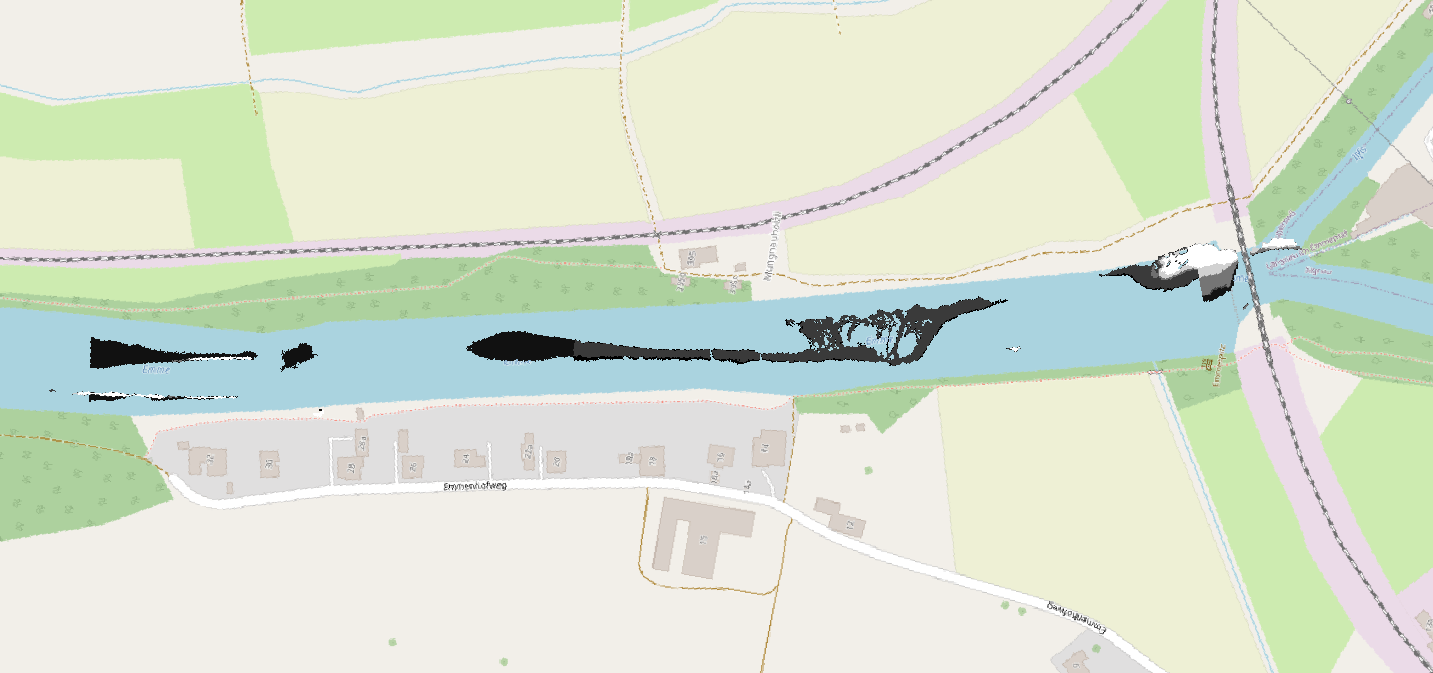
\includegraphics[width=\textwidth]{Bilder/variable_tributary_caused.png}
		\caption{Variable, tributary-caused. Coloring indicates variability, 
			and the patch lies adjacent to a tributary inflow.}
		\label{fig:cwp_variable_tributary}
	\end{subfigure}
	\hfill
	\begin{subfigure}[t]{0.48\textwidth}
		\centering
		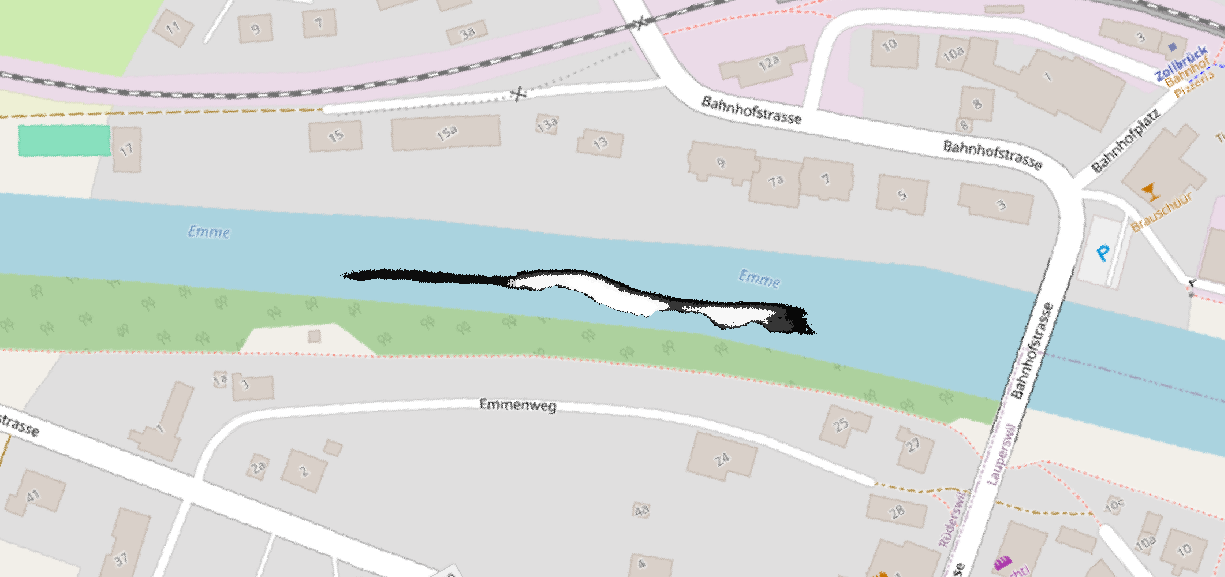
\includegraphics[width=\textwidth]{Bilder/variable_non_tributary_caused.png}
		\caption{Variable, non-tributary-caused. Coloring indicates 
			variability, but no tributary inflow is present nearby.}
		\label{fig:cwp_variable_nontributary}
	\end{subfigure}
	
	\vspace{0.5cm}
	
	\begin{subfigure}[t]{0.48\textwidth}
		\centering
		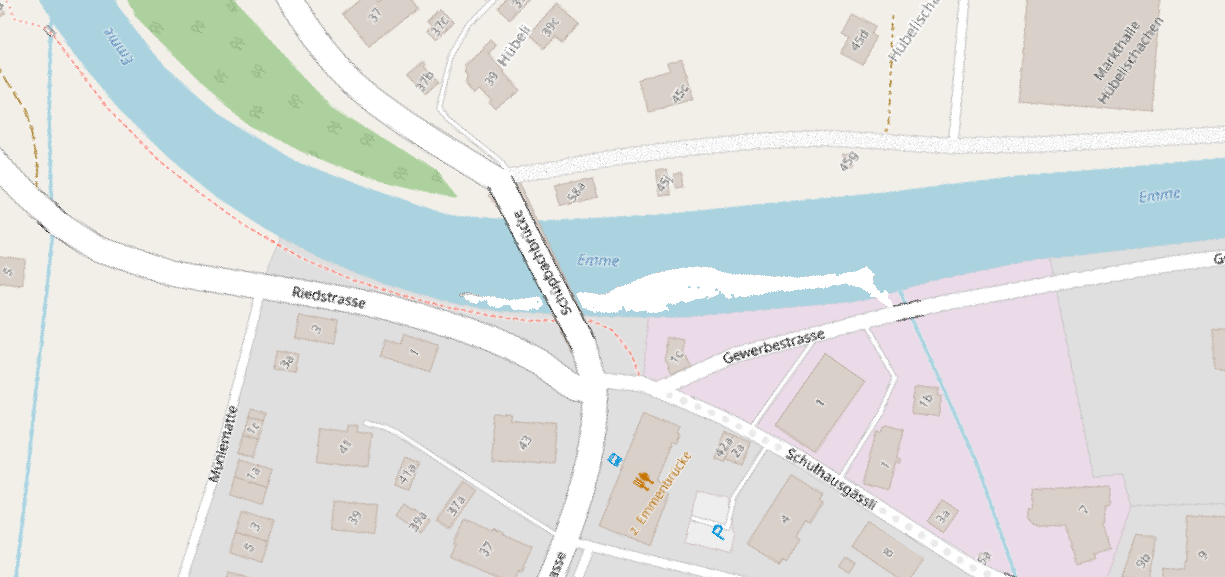
\includegraphics[width=\textwidth]{Bilder/non_variable_tributary_caused.png}
		\caption{Non-variable, tributary-caused. The patch shows little 
			variability in the fuzzy overlay despite proximity to a 
			tributary inflow.}
		\label{fig:cwp_nonvariable_tributary}
	\end{subfigure}
	\hfill
	\begin{subfigure}[t]{0.48\textwidth}
		\centering
		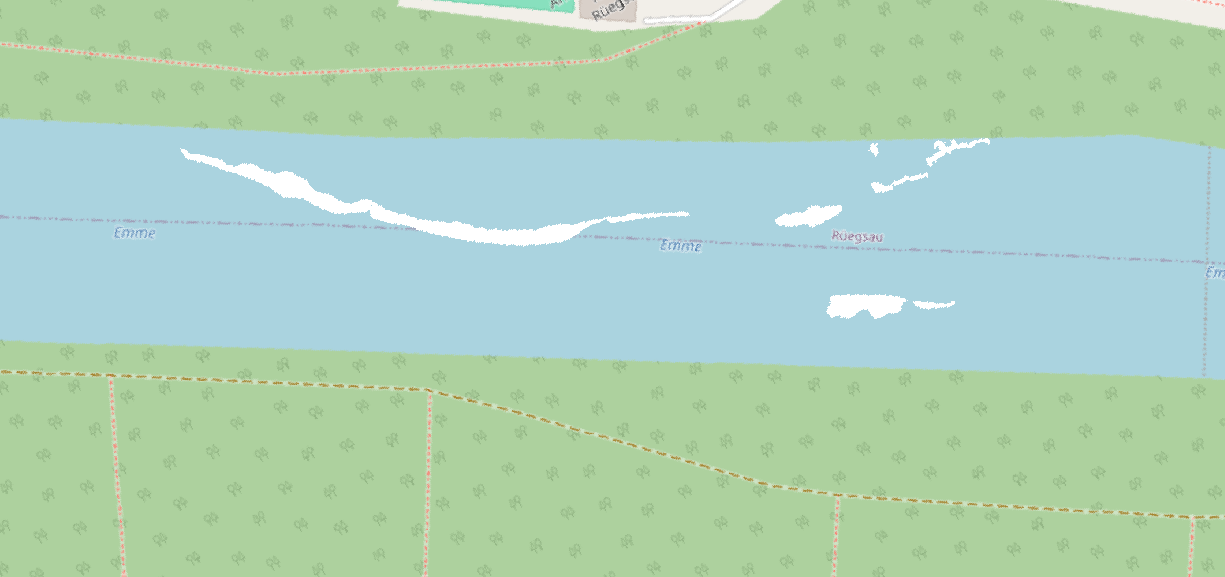
\includegraphics[width=\textwidth]{Bilder/non_variable_non_tributary_caused.png}
		\caption{Non-variable, non-tributary-caused. The patch shows little 
			variability and no tributary inflow is present nearby.}
		\label{fig:cwp_nonvariable_nontributary}
	\end{subfigure}
	
	\caption{Examples of the four classification outcomes from the decision 
		tree in Figure~\ref{fig:decision_tree_classification}: variable vs. 
		non-variable patches (rows), further split by tributary attribution 
		(columns).}
	\label{fig:cwp_classification_examples}
\end{figure}

% TODO: reference to the appendix, where a grid of all CWP and their 
%        classification is provided

\subsection{Computing Morris Sensitivity Indices with respect to CWP Area}
\label{sec:morris_indices}

With the 24 CWPs classified, the second stage quantifies their sensitivity 
to buffer pixel count, step length, and temperature delta. Following 
\citet{lilburne_sensitivity_2009}, the spatially distributed polygon output 
is aggregated to a scalar statistic per run -- here, the total detected CWP 
area within each bounding box. Figure~\ref{fig:cwp_stats_overview} 
summarises the steps involved.

\begin{figure}[H]
	\centering
	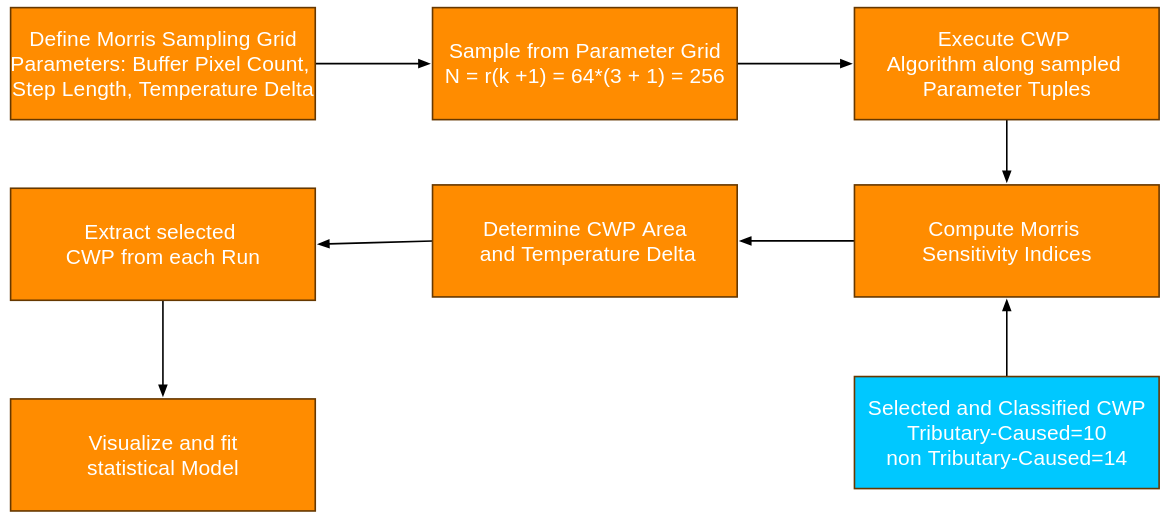
\includegraphics[width=\textwidth]{Bilder/cwp_stats.png}
	\caption{Visual overview of the steps involved in computing Morris 
		sensitivity indices with respect to CWP area: setting up the second 
		Morris experiment ($k=3$) and executing the algorithm across the sampled 
		parameter tuples, computing lumped area statistics per annotated CWP 
		location and Morris run, and computing and visualising the Morris 
		sensitivity indices.}
	\label{fig:cwp_stats_overview}
\end{figure}

\subsubsection{Setting up Second Sampling Grid and Executing Algorithm}

A three-dimensional Morris sampling grid spanning buffer pixel count, step 
length, and temperature delta was set up, as depicted in 
Figure~\ref{fig:morris_grid_second}. A total of 64 trajectories were sampled 
($r = 64$), yielding $64 \times (3+1) = 256$ parameter tuples 
(Equation~\ref{eq:morris_runs}). The algorithm was executed in parallel using 
the same orchestration as in Section~\ref{sec:modeleval}, with the remaining 
parameters held constant as listed in Table~\ref{tab:held_constant_second_morris}.

\begin{figure}[H]
	\centering
	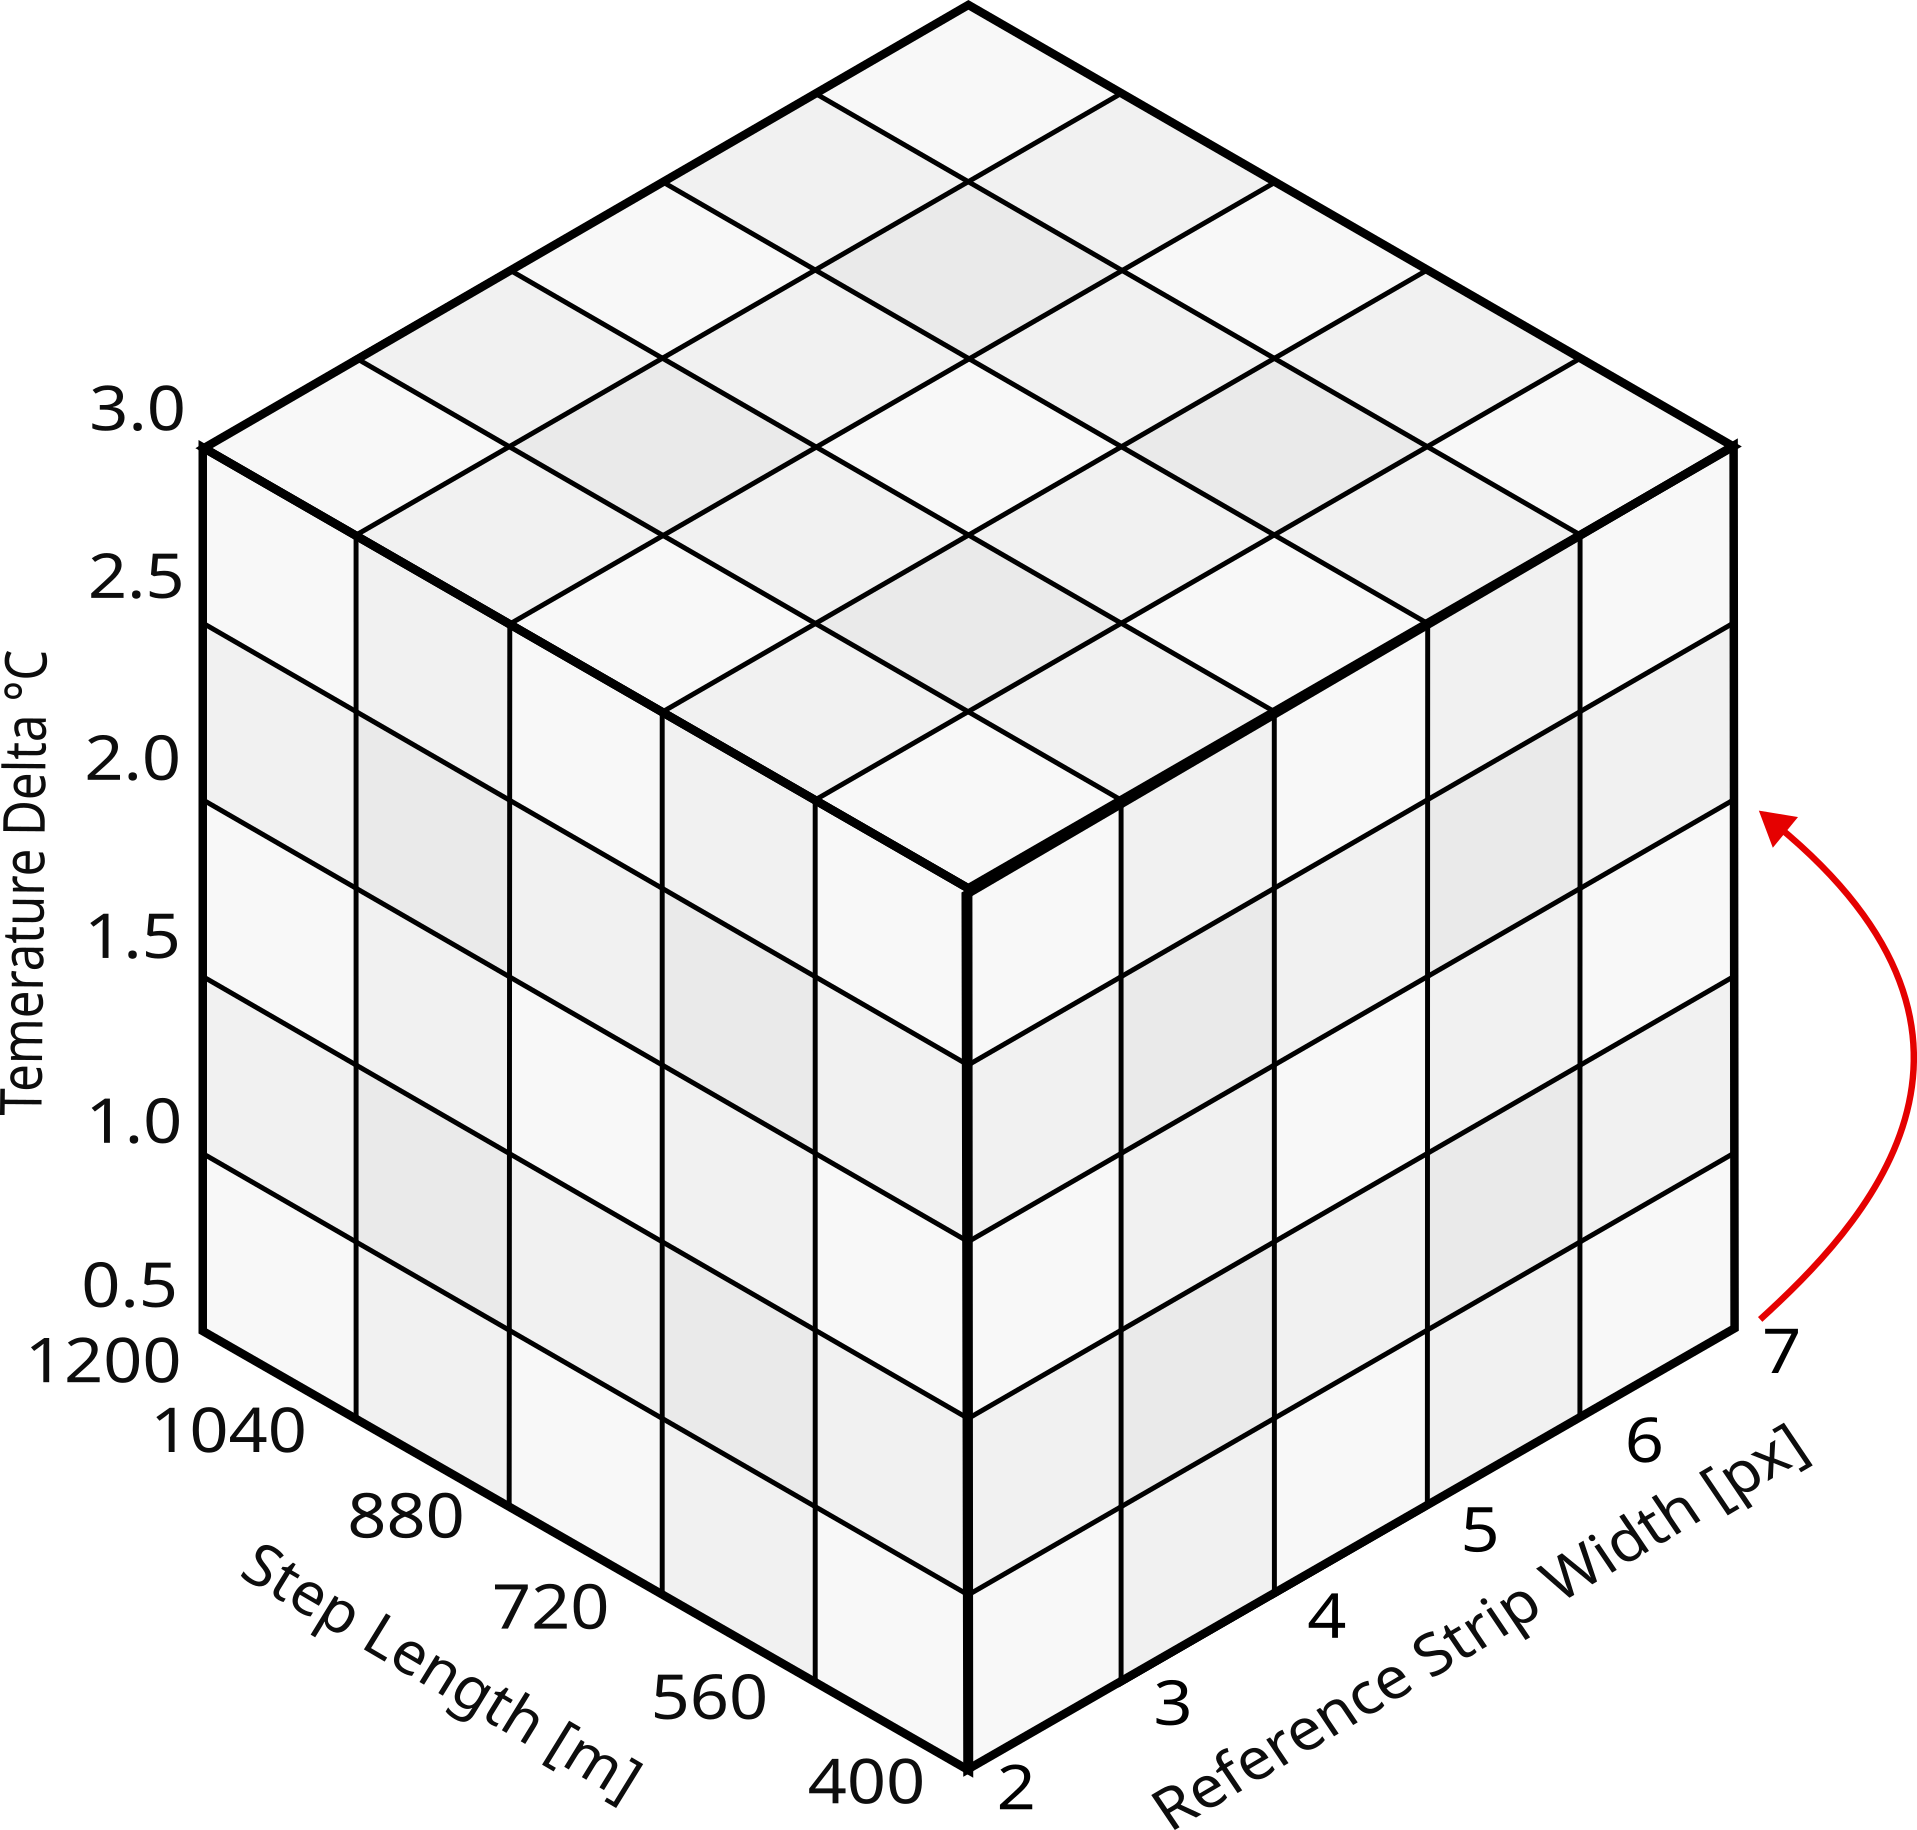
\includegraphics[width=0.8\textwidth]{Bilder/large_moris_grid_image.png}
	\caption{Visual depiction of the second Morris sampling grid, spanning step 
		length, buffer pixel count, and the temperature delta threshold. The red 
		arrow indicates the $\Delta$ chosen.}
	\label{fig:morris_grid_second}
\end{figure}

\begin{table}[H]
	\centering
	\caption{Parameter values held constant during the second Morris experiment, 
		while \texttt{step\_length}, \texttt{buffer\_px}, and \texttt{delta\_T} 
		were varied.}
	\label{tab:held_constant_second_morris}
	\begin{tabular}{lr}
		\toprule
		Parameter & Value \\
		\midrule
		\texttt{min\_patch\_area\_m2} & 2 m$^2$ \\
		\texttt{zone\_halfwidth\_m}   & 60 m \\
		\texttt{connect\_diagonals}   & TRUE \\
		\bottomrule
	\end{tabular}
\end{table}

\subsubsection{Computing Lumped Statistics for the Selected CWPs}

For each of the 24 annotated bounding boxes and each Morris run, the CWP 
polygons inside the bounding box are extracted and the total detected CWP 
area and the area-weighted temperature delta are computed. If no CWP is 
detected for a given run, both statistics are set to zero. 
Figure~\ref{fig:cwp_lumping_decision} illustrates this computation.

\begin{figure}[H]
	\centering
	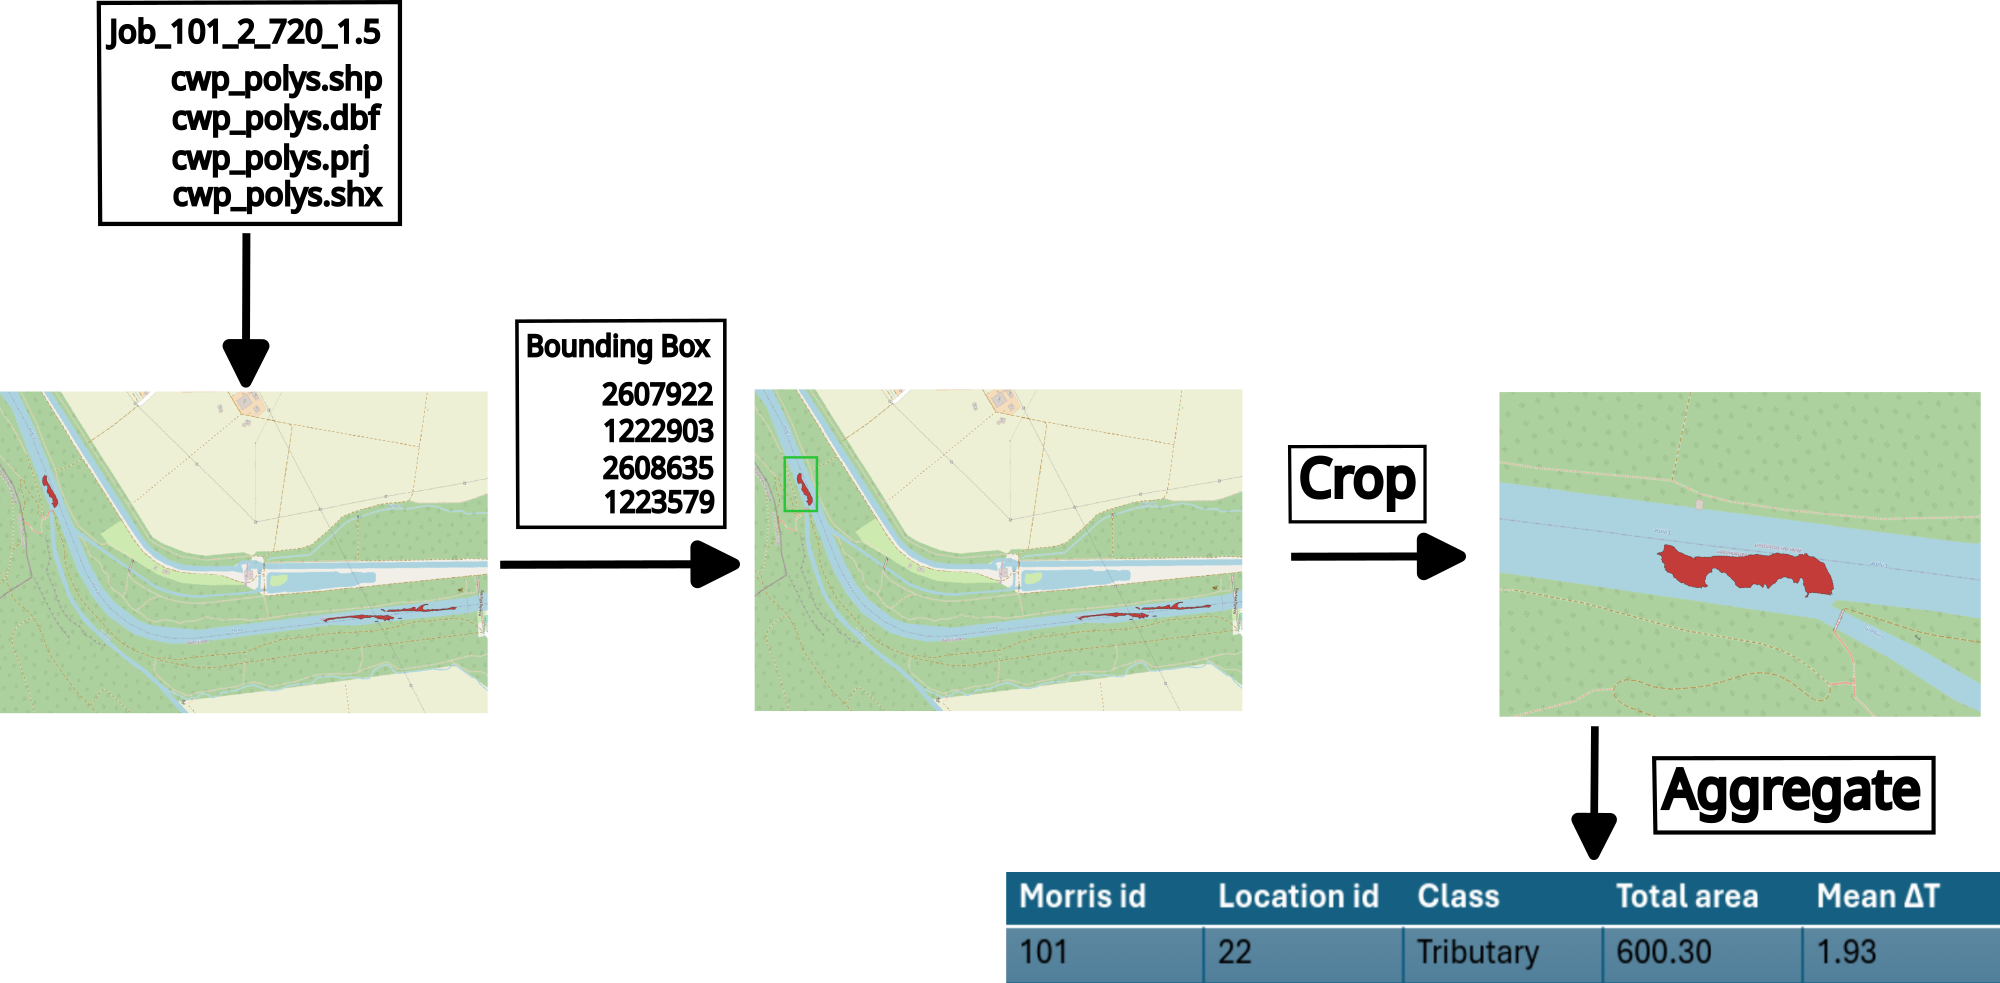
\includegraphics[width=\textwidth]{Bilder/cropping_strat_img.png}
	\caption{Schematic overview of the lumped-statistics computation for one 
		annotated CWP location (Limpbach inflow into the Emme near Utzenstorf BE). 
		For each Morris run, CWP polygons are cropped to the bounding box; if 
		polygons are present, total area and area-weighted mean temperature delta 
		are computed; if the bounding box is empty, both are set to zero.}
	\label{fig:cwp_lumping_decision}
\end{figure}

The result is a table in which each row corresponds to one annotated location 
under one parameter tuple. Table~\ref{tab:lumped_stats_example} shows an excerpt; 
the varying area values across rows sharing the same location confirm that total 
CWP area is a suitable scalar statistic for characterising parameter sensitivity.

\begin{table}[H]
	\centering
	\caption{Excerpt of the lumped statistics table. Each row corresponds to one 
		annotated CWP location under one Morris parameter tuple.}
	\label{tab:lumped_stats_example}
	\begin{tabular}{lcrr}
		\toprule
		Location & Class & $\Delta T$ [$^{\circ}$C] & Total CWP area [m$^2$] \\
		\midrule
		2 & Non-tributary & 3.67 & 32.32 \\
		2 & Non-tributary & 4.13 & 22.65 \\
		2 & Non-tributary & 4.28 & 18.92 \\
		$\vdots$ & $\vdots$ & $\vdots$ & $\vdots$ \\
		4 & Tributary & 2.40 & 39.82 \\
		4 & Tributary & 2.91 & 15.89 \\
		4 & Tributary & 0    & 0  \\
		$\vdots$ & $\vdots$ & $\vdots$ & $\vdots$ \\
		\bottomrule
	\end{tabular}
\end{table}

\subsubsection{Computing Morris Sensitivity Indices}

Before computing the sensitivity indices, the total CWP area values are 
normalised per location using min-max scaling into $[0, 1]$. This ensures 
comparability across locations: without normalisation, locations with 
inherently larger CWP would produce larger absolute area differences, 
inflating their sensitivity indices relative to smaller patches. After 
scaling, a value of 1 corresponds to the maximum area detected for that 
location across all runs and a value of 0 to an empty bounding box.

The Morris indices $\mu$, $\mu^*$, and $\sigma$ are then computed with 
respect to the normalised area values using the R package 
\texttt{sensitivity}.

% TODO: briefly describe on a high level how tell() works in the sensitivity package

\subsubsection{Visualisation and Statistical Modelling}
\label{sec:morris_viz_model}

Two sets of boxplot visualisations were produced. The first displays $\mu^*$ 
and $\sigma$ with respect to step length, stratified by CWP class, to allow 
a direct comparison of sensitivity between tributary-caused and 
non-tributary-caused CWPs. The second displays $\mu^*$ for all three varied 
parameters pooled across both classes, providing an overview of their relative 
influence on CWP area.

Additionally, a linear model was fitted to assess whether CWP area and 
temperature delta are associated with step-length sensitivity:

\begin{equation}
	\mu^*_{\text{step length}} = \beta_0 + \beta_1 \cdot \overline{\text{area}} 
	+ \beta_2 \cdot \overline{\Delta T} + \varepsilon
	\label{eq:linear_model}
\end{equation}

where $\mu^*_{\text{step length}}$ is the Morris sensitivity index for step 
length, $\overline{\text{area}}$ and $\overline{\Delta T}$ are the mean total 
CWP area and mean temperature delta across all Morris runs for each annotated 
location, and $\varepsilon$ is the residual error. The model was fitted using 
R's \texttt{lm()} across all 24 locations, pooling both classes.


\section{Addressing Research Question 3: Algorithm Modification}
\label{sec:rq3_methods}

Building on the sensitivity analysis findings of 
\citet{tonolla_thermische-kartographie_2026}, this section describes the 
design and implementation of a modified algorithm, referred to as v3, that 
addresses the identified parameter sensitivities. The section covers the 
motivation for each design decision, the operationalisation of the revised 
reference temperature computation, the implementation details, and the 
resulting reduction in free parameters.

\subsection{Motivation for Algorithm Modification}

The sensitivity analysis of \citet{tonolla_thermische-kartographie_2026} provides 
direct motivation for the design of v3. Three findings from that work informed 
specific algorithmic decisions.

First, \citet{tonolla_thermische-kartographie_2026} found that the buffer pixel 
count has little influence on the detected CWP area. This suggests that the buffer 
pixel count qualifies as a candidate for factor fixing -- that is, it can be set 
to a fixed constant and removed as a free parameter without meaningfully affecting 
the algorithm's output. In v3, the buffer pixel count is therefore internalized 
and set to a constant value of 3, which lies within the range of values examined 
by \citet{tonolla_thermische-kartographie_2026}.

Second, \citet{tonolla_thermische-kartographie_2026} identified the step length 
parameter as having a non-negligible influence on the detected CWP area. A 
plausible mechanistic explanation for this sensitivity is that CWPs spanning a 
slab boundary are compared against two different reference temperatures -- one 
per slab -- which can produce artificial truncations in the detected patch extent. 
This motivated a fundamental redesign of the reference temperature computation in 
v3, replacing the slab-based approach with a spatially continuous IDW-based scheme 
that does not depend on a step length parameter at all.

Third, \citet{tonolla_thermische-kartographie_2026} found the temperature delta 
parameter to be the most influential of the parameters examined. Unlike the buffer 
pixel count and step length, however, the temperature delta cannot simply be 
removed: different thresholds are used in the literature to define CWPs 
\citep{casas-mulet_unmanned_2020}, and the user must therefore retain the ability 
to set it according to their chosen definition. The temperature delta is 
accordingly retained as a free parameter in v3.

Whether the design decisions described above are supported by the Morris screening 
analysis conducted in this work will be examined in the Results and Discussion.

\subsection{Operationalisation of Surrounding Stream Temperature}

The step-length dependency was addressed by rethinking the operationalisation of 
the surrounding stream temperature used as the reference for pixel flagging. In 
v1 and v2, the reference temperature for each pixel is determined by the median 
temperature of the slab segment to which that pixel belongs. This approach has 
two consequences: it requires a user-defined step length, and it produces a 
reference temperature field that is piecewise constant -- uniform within each 
slab and discontinuous at slab boundaries. CWPs that happen to span a slab 
boundary are therefore compared against two different reference temperatures, 
which can produce artificial cutoffs in the detected patch extent.

In v3, this is replaced by an inverse distance weighting (IDW) scheme. Rather 
than dividing the reach into fixed slabs, reference temperature sample points 
are obtained by sampling multiple step length values from a uniform distribution 
and extracting the median temperature at each resulting segment's visual center. 
These sample points, pooled across all sampled step lengths, are then used to 
compute a spatially continuous reference temperature raster via IDW, where each 
cell's reference temperature is a distance-weighted average of the surrounding 
sample point temperatures. This guarantees that the reference temperature is a 
spatially continuous field, and that no sharp cutoffs at slab boundaries can 
occur.

\subsection{Implementation Detail}

The implementation of v3 follows the structure of v2 closely, differing only in 
the computation of the reference temperature raster (steps 1--5 below, replacing 
steps 1--5 of Table~\ref{tab:cwp_pseudocode}). The full reference temperature 
computation proceeds as follows:

\begin{table}[H]
	\centering
	\caption{High-level overview of the v3 CWP detection algorithm. Steps 1--5 
		replace the corresponding steps of Table~\ref{tab:cwp_pseudocode}; 
		steps 6--8 are identical to v2.}
	\label{tab:cwp_pseudocode_v3}
	\begin{tabular}{@{}c p{11.5cm}@{}}
		\toprule
		\textbf{Step} & \textbf{Description} \\
		\midrule
		1 & Sample 20 candidate step length values from a uniform distribution 
		with bounds 500--3000 metres. \\
		\addlinespace
		2 & For each candidate step length, divide the river centerline into $n$ 
		segments; construct a narrow 3-pixel-wide reference strip polygon for 
		each segment; extract the median temperature of each segment from the 
		TIR raster; compute the visual centre of each strip polygon and assign 
		the corresponding median temperature to this point. \\
		\addlinespace
		3 & Pool the reference points (location + temperature) from all 20 step 
		length values into a single combined set of IDW sample points. \\
		\addlinespace
		4 & Initialise a new raster with the same extent and resolution as the 
		TIR raster. For each cell: if the corresponding TIR cell is 
		\texttt{NaN}, set to \texttt{NaN}; otherwise compute a 
		distance-weighted reference temperature via IDW over the pooled 
		sample points, using a decay power of 2. \\
		\addlinespace
		5 & Round the TIR raster using a fixed rounding factor. \\
		\addlinespace
		6 & Subtract the rounded TIR raster from the reference raster; flag 
		pixels where the difference exceeds $\Delta T$, producing a binary 
		CWP raster. \\
		\addlinespace
		7 & Polygonize the binary CWP raster into patch polygons. \\
		\addlinespace
		8 & Filter patches by minimum area; compute per-patch temperature 
		statistics; apply a patch-level threshold check against the reference 
		temperature. \\
		\bottomrule
	\end{tabular}
\end{table}

Step 4 is implemented in C++ and imported into R via the \texttt{Rcpp} package, 
as the per-pixel IDW computation was identified as the primary computational 
bottleneck.

\subsection{Reduction of Parameters}

The buffer pixel count is fixed internally at a value of 3. The step 
length parameter is no longer required, as the IDW reference temperature 
computation samples reference points across a range of step lengths. The 
zone halfwidth parameter is likewise no longer needed, as the extent of 
the reference raster is matched to the extent of valid TIR pixels -- 
though this implies a constraint: v3 requires a TIR raster with an exact 
water mask, with non-river pixels set to \texttt{NaN}. The remaining free 
parameters are: the TIR raster and centerline paths, minimum patch area, 
rounding factor, temperature delta threshold, and diagonal connectivity.

\section{Usage of AI}

The large language models Claude Sonnet 4.6 and Claude Opus 4.6 (Anthropic) 
were used as aids in this project. Detailed insight into the usage is given 
in Appendix A.
	\chapter{Results}

\section{Comparison of outputs}

% this should show images showing the new version and the old version of the cwp algorithm and how the outputs generally allign but are not pixel perfect. Tree images are sufficient. Just to provide some interpretation. 

% somewhere the jackard similarity should also be stated. I just do not know where yet. Maybe in the plot description, maybe somewhere else in a table


% the jaccard similarities are
% 0.936, 0.9555, 0.9563


% Here I simply provide the resulting boxplot diagrams -> Should be four in total. For every parameter and for every lumped statistic. Additionally it could also be of interest to plot the results with respect to patch size and stuff like this, so digging a bit deeper to uncover patters that could be interestin

The three comparison runs achieved outputs that are in general aggrement of the cwp location and shape but are not on a pixel perfect basis. The jaccard similarities for the three runs are 0.936, 0.956 and 0.976 which shows generally good agreement between the methods. 

Figure \ref{fig:param_combi_3_general_agreement} shows the cwps generated during trial run 3. In red the polygons of the speed optimized algorithm, in red the polygons of the original algorithm. It can be seen that for the displayed cwps, the two algorithms are in generall agreement, however do not fully agree on the pixel level. Figure xzz shows a more pronounced version of this disagreement.



\begin{figure}[H]
	\centering
	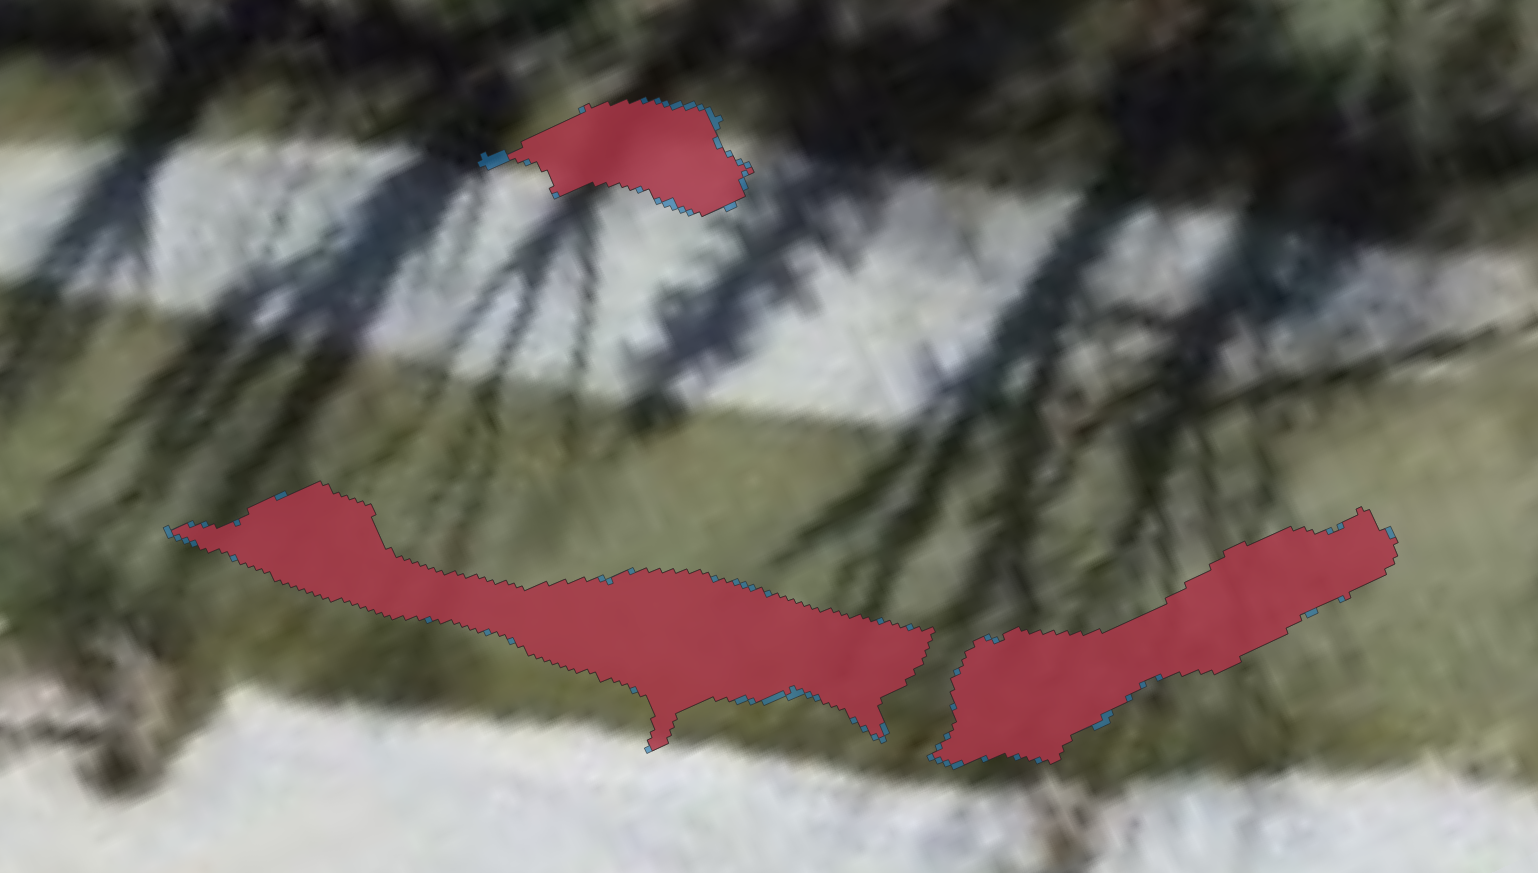
\includegraphics[width=\textwidth]{Bilder/param_combi_3_general_agreement.png}
	\caption{CWPs generated during trial run 3. Polygons of the speed-optimized algorithm are shown in red, and polygons of the original algorithm are shown in blue. The two algorithms are in general agreement, but do not fully agree at the pixel level.}
	\label{fig:param_combi_3_general_agreement}
\end{figure}

Figure \ref{fig:trial_run_1_more_pronounced_dis} shows an example of more pronounced disagreement between the two functions for trial run 1, figure \ref{fig:trial_run_perfect_agreement} shows an example set of cwps with perfect agreement between the two methods

\begin{figure}[H]
	\centering
	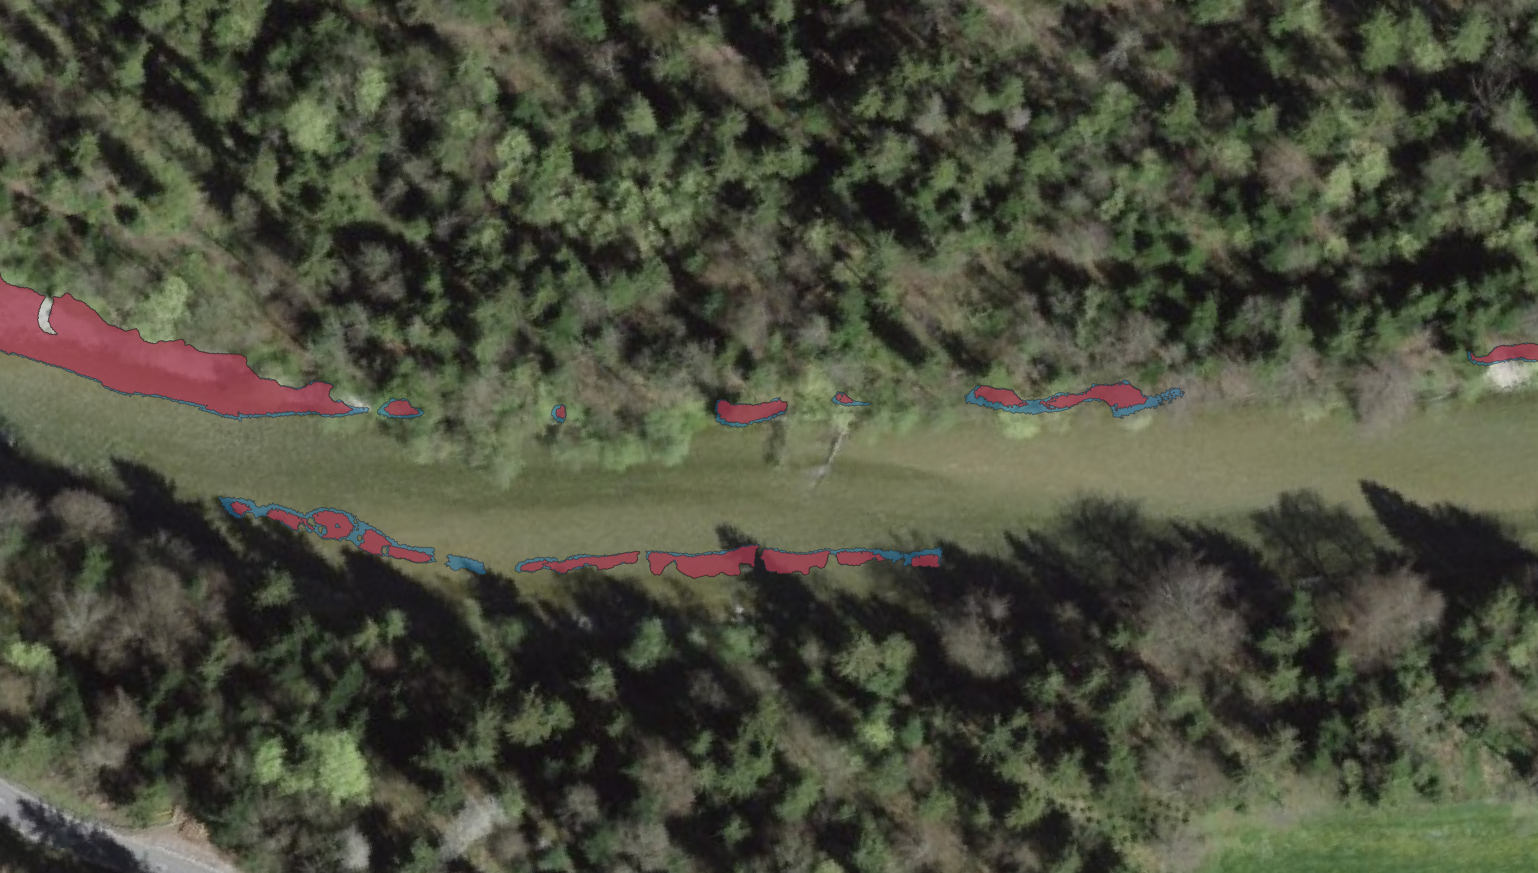
\includegraphics[width=\textwidth]{Bilder/trial_run_1_more_pronounced_dis.png}
	\caption{TODO}
	\label{fig:trial_run_1_more_pronounced_dis}
\end{figure}

\begin{figure}[H]
	\centering
	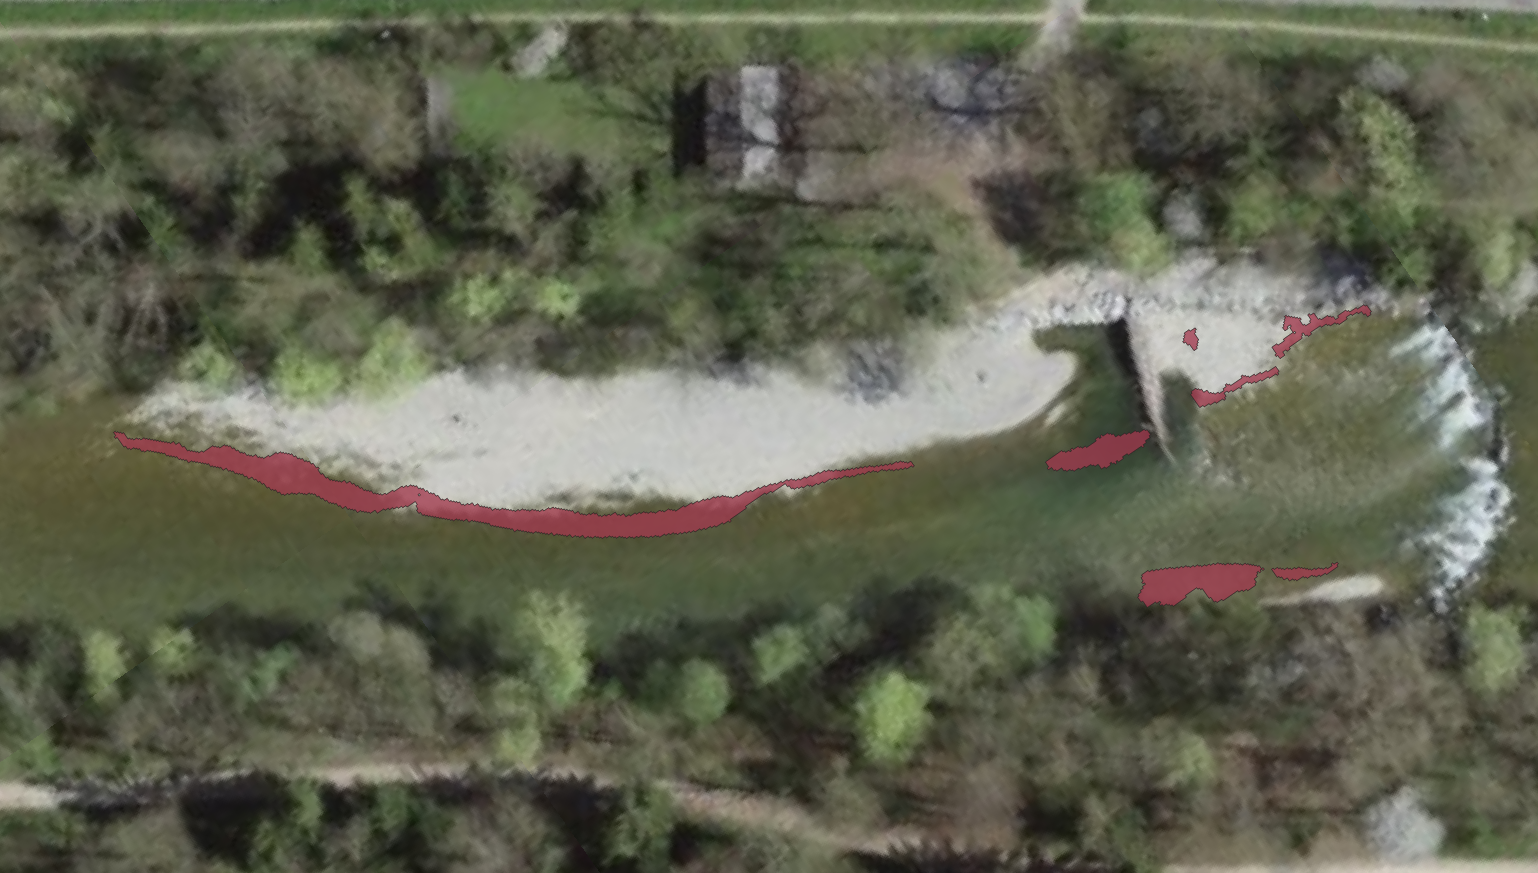
\includegraphics[width=\textwidth]{Bilder/trial_run_perfect_agreement.png}
	\caption{TODO}
	\label{fig:trial_run_perfect_agreement}
\end{figure}





\section{Speed comparison in execution}

% a simple line plot showing two lines with different collor. On the x-axis the step length, on the y axis execution time. One line is the execution speed of the optimized algorithm, the other line is the execution speed of the non optimized algorithm.

% It should be visible that the execution time of the new algorithm is shorter and generally constant over the step length parameter. The older version is slower and scales to longer execution speeds for smaller step lengths.

Figure \ref{fig:speed_comparison} shows the execution speed of the original aswell as the speed optimized cwp function. On the y-axis the execution speed in hours is ploted, on the x-axis the step-length parameter is ploted in meters. Execution speed is a constant half hour for teh speed optimized version where the original function ranges between 2 and 1.25 hours for the three runs whith hihger exeuction times for shorter step lengths.


\begin{figure}[ht]
	\centering
	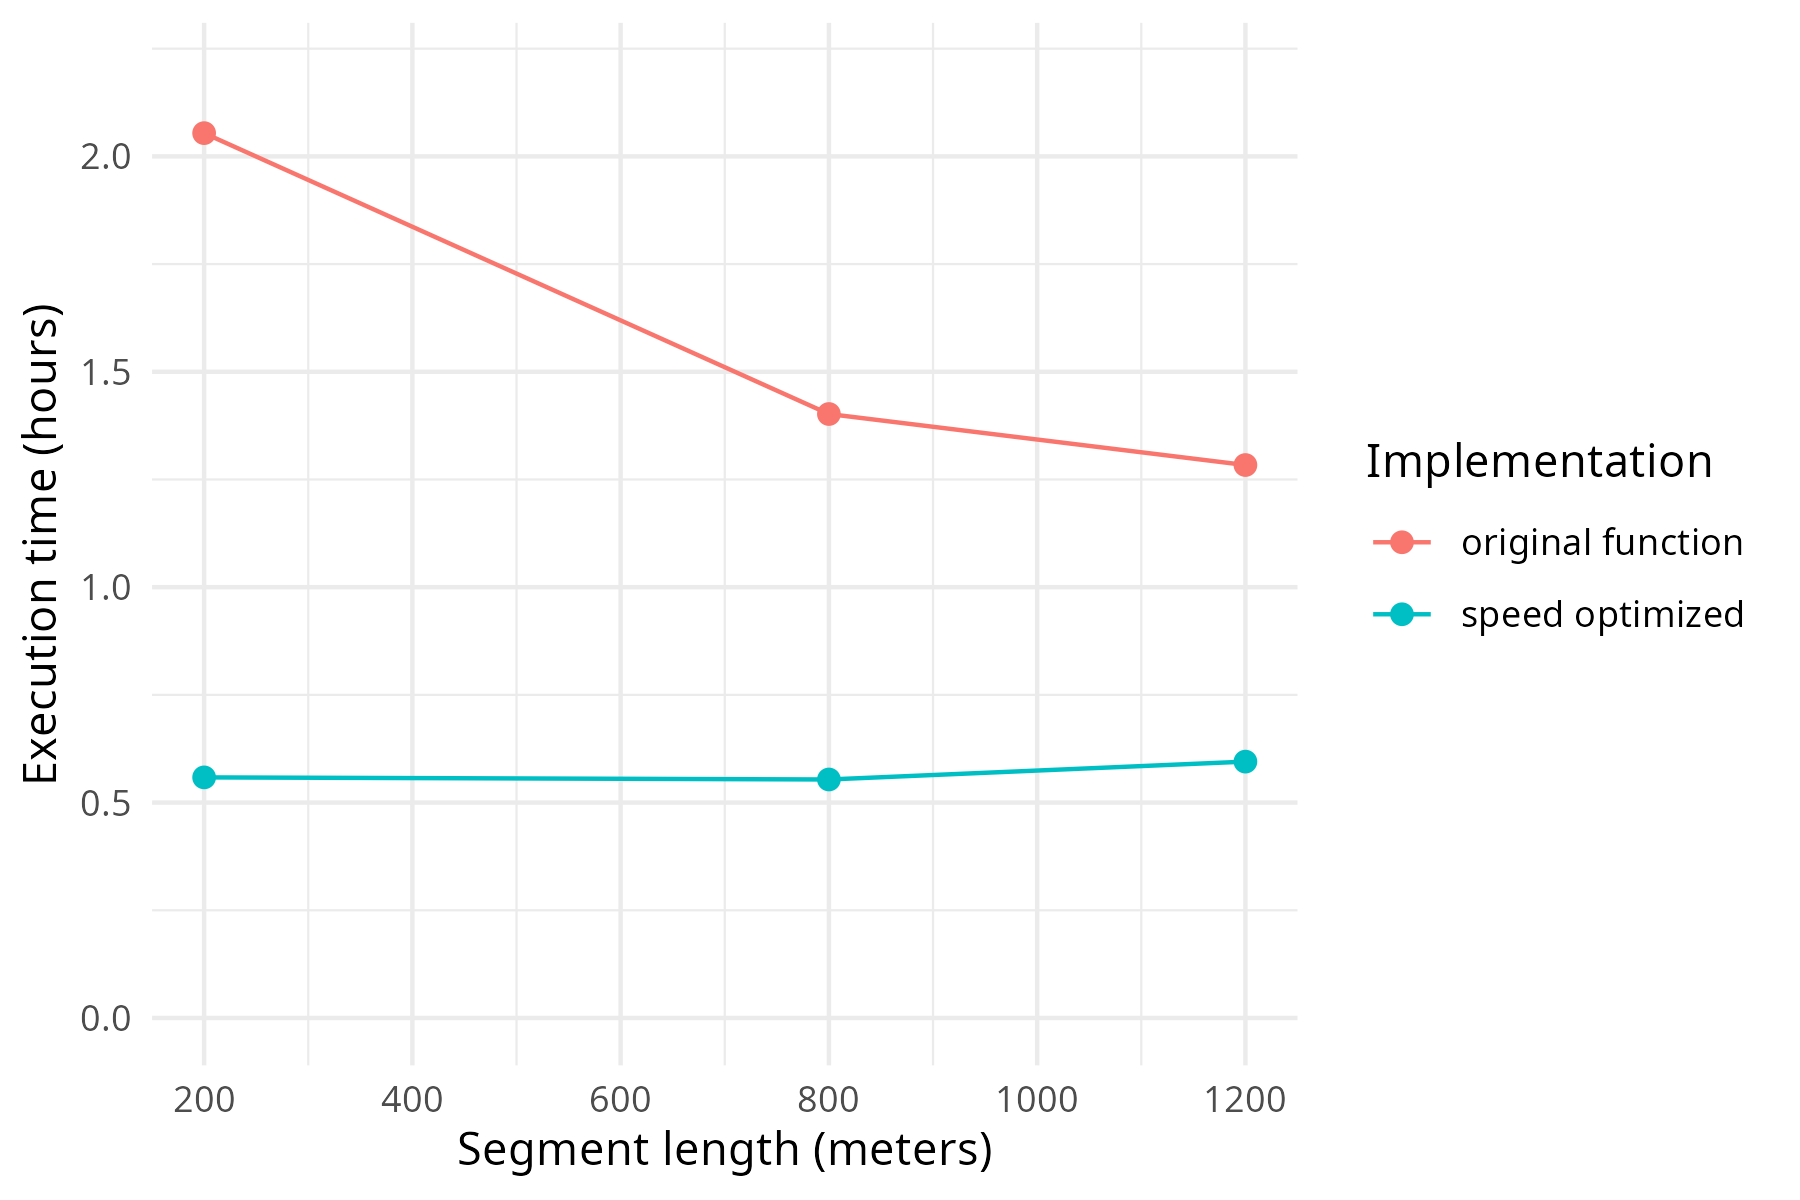
\includegraphics[width=0.8\textwidth]{Bilder/speed_comparison.png}
	\caption{Execution time of the original (v1) and optimized (v2) implementations of \texttt{detect\_cwp\_single} as a function of segment length. The optimized implementation shows execution times that are both shorter and largely constant across segment lengths, whereas the original implementation scales disproportionately with decreasing segment length (i.e., increasing number of segments).}
	\label{fig:speed_comparison}
\end{figure}




\section{Sensitiviy scores for step length parameter}

% include a plot of mu star and sigma for the non tributary caused and the tributary caused cold water patches. Also briefly introduce what is visible on the plot. 

% the plot shows boxplots of the mu.star and sigma sensitivity parameters for the xyz classified cold water patches. Red shows the tributary caused, blue the non tributary caused cold water patches. On the


Figure \ref{fig:step_length_sensitivity} shows morris sensitivity indices sigma and mustar with regards to the step length parameter. It can be seen that all non tributary caues CWP have a sensitivity index below 0.2. The spread in mu star for the sensitivity caused cwp is larger with some cwp featuring a similar sensitivity as the non tributary caused cwp and some featuing a substantially larger sensitivity value ( 0.3 and 0.6). The mean of both mu.star boxplots are very similar for both classes. 

\begin{figure}[ht]
	\centering
	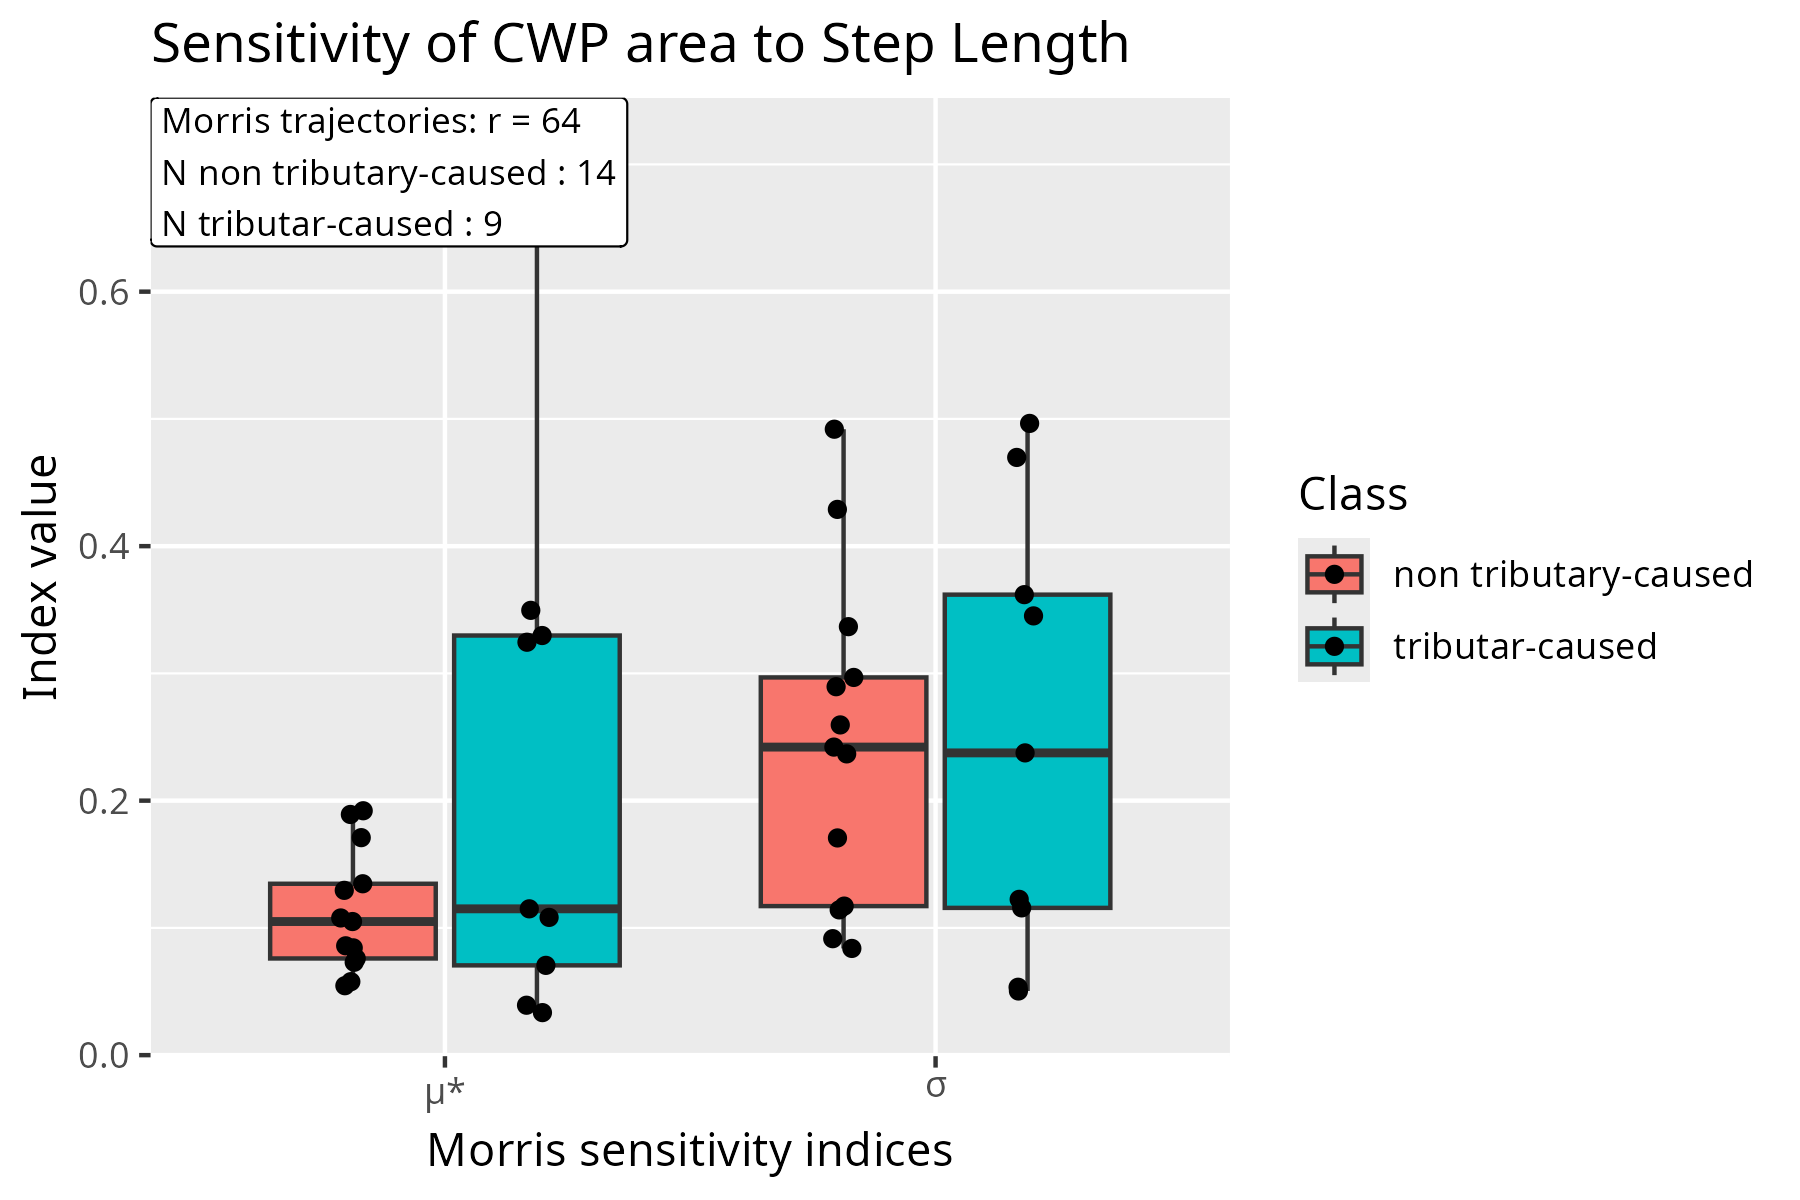
\includegraphics[width=0.8\textwidth]{Bilder/step_length_results.png}
	\caption{Morris sensitivity indices ($\mu^*$ and $\sigma$) for the \texttt{step\_length} parameter with respect to cold water patch area, stratified by patch class (red: tributary-caused; blue: non-tributary-caused). Boxplots show the distribution across bounding boxes, with sample sizes ($n$) given below each box.}
	\label{fig:step_length_sensitivity}
\end{figure}

\newpage

\section{Mu star for all parameters over all CWP}

% inlclude a plot of mu star for buffer bixels delta_T and also the step length for all cwp. Describe what the plot shows.

% the plot shows boxplots if mu star for the three different parameters buffer px, delta_T and also step length for all classified cwp. Each boxplot shows the distribution of the different mu.star values per location/area.


% further subsections are needed here for shure. Because in the discussion for instance i am also going to address the fact, that i think only the large tributary cwp are realy affected by this issue.

Figure \ref{fig:mu_star_overall} displays the mu.star values of all cwp with respect to the three different parameters varied during the morris experiment. The buffer pixel count continuously scores very low mu.star values while the step length and the temperature delta deviate from zero. Especially the temperature delta seems to highly influence the cwp with respect to their area.

\begin{figure}[ht]
	\centering
	
\includegraphics[width=0.8\textwidth]{Bilder/mu_star_res.png}
	\caption{Overall $\mu^*$ sensitivity indices for \texttt{buffer\_px}, \texttt{delta\_T}, and \texttt{step\_length} across all classified cold water patches ($N = 24$ locations, $r = 64$ trajectories).}
	\label{fig:mu_star_overall}
\end{figure}


\section{Mu.star and size for every cwp}

% include a plot showing mu.star in one axis and on the other axis the size of the cwp. Color the dots after the group membership. The large tributary caused patches should also have a large mu.star where smaller tributary caused patches might have a smaller mu star.


Figure  \ref{fig:mu_star_vs_area} shows the 24 selected cpw along 3 different dimensions. On the x axis, the averaged cwp area over all morris runs is depicted, on the y axis the sensitivty against the step length parameter is depicted. The color is used to indicate the average temperature delta to the surrounding environment averaged over all morris runs is depicted. The shape is indicating the class of the cwp.

\begin{figure}[ht]
	\centering
	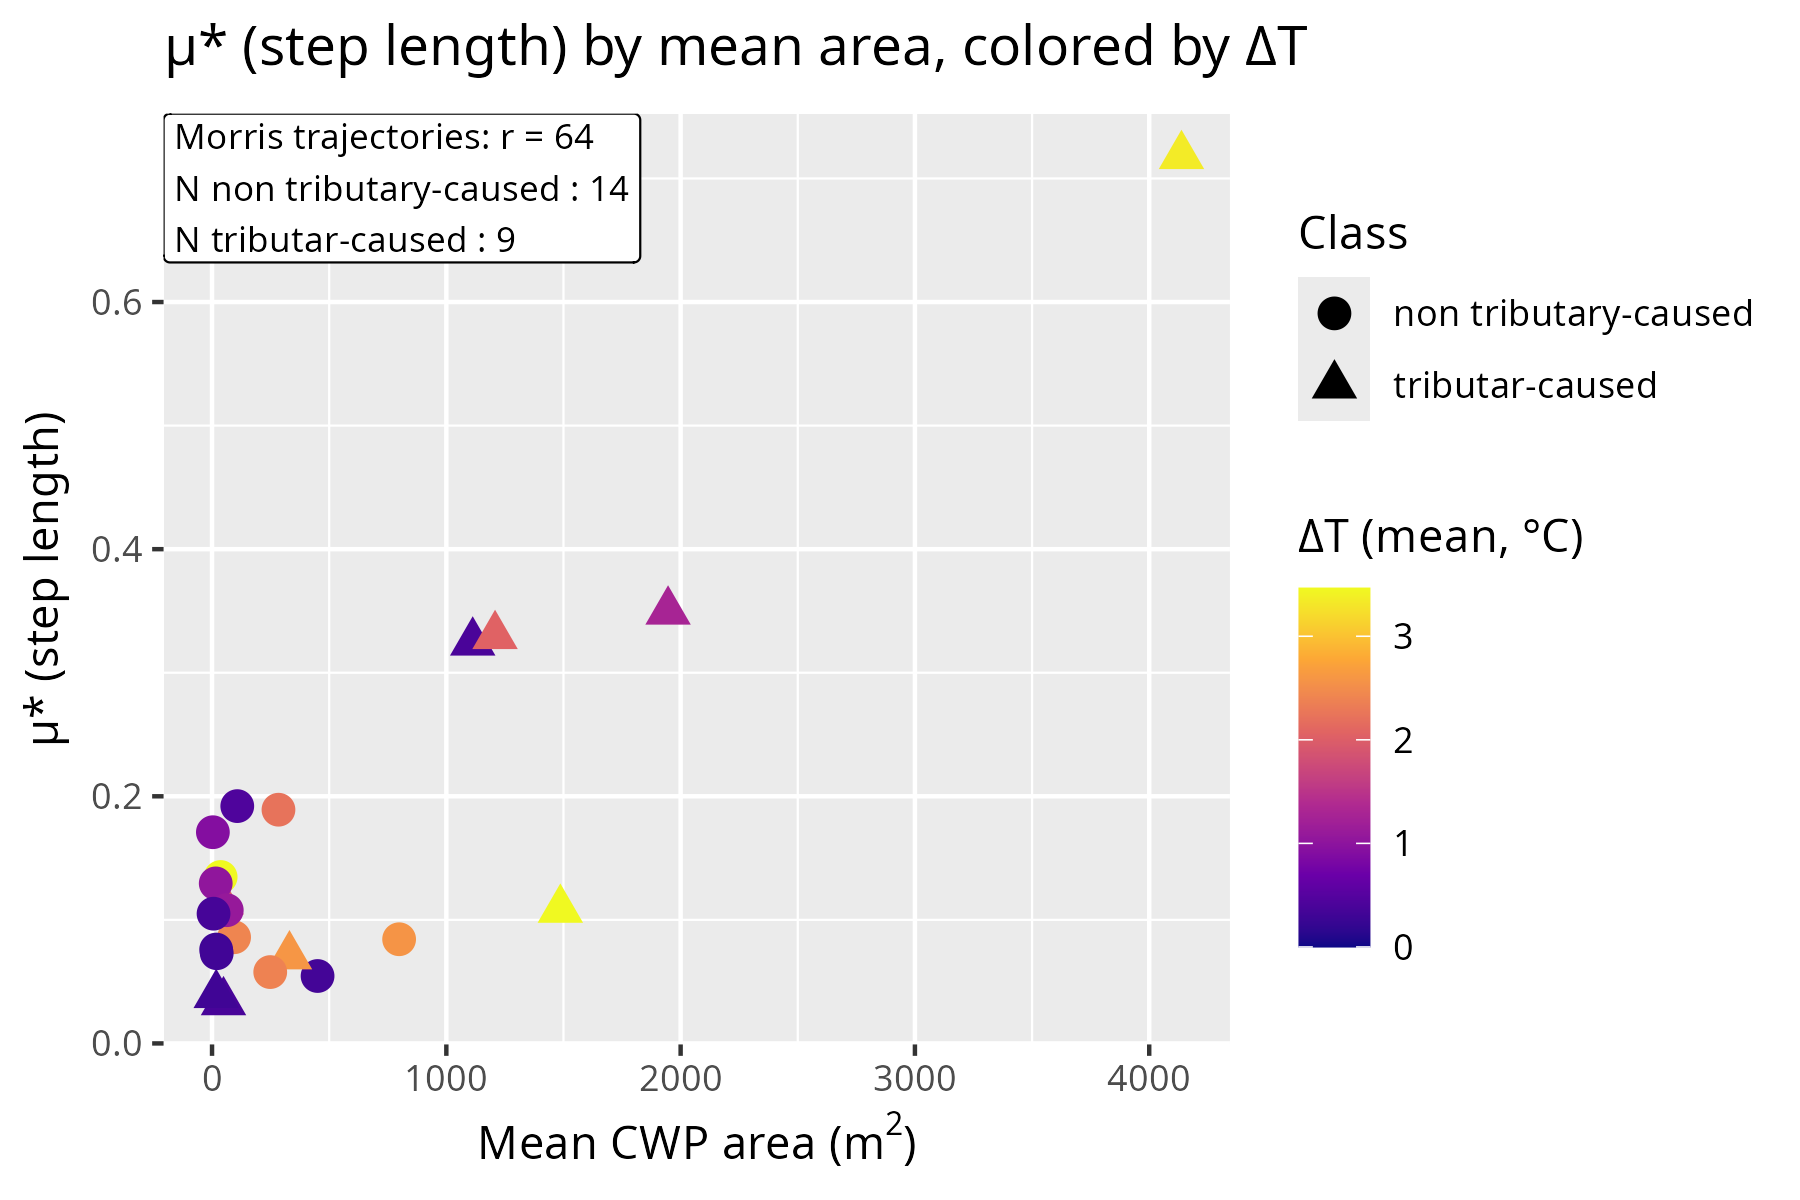
\includegraphics[width=0.8\textwidth]{Bilder/mu_star_vs_area_vs_deltaT.png}
	\caption{$\mu^*$ (step length) versus mean CWP area for each annotated location, colored by patch class.}
	\label{fig:mu_star_vs_area}
\end{figure}


\begin{table}[h]
	\centering
	\caption{Regression results for $\mu^*$ predicted by mean area and mean $\Delta T$}
	\label{tab:regression_mustar}
	\begin{tabular}{lrrrr}
		\toprule
		Predictor & Estimate & SE & $t$ & $p$ \\
		\midrule
		(Intercept)        & $9.024 \times 10^{-2}$  & $3.094 \times 10^{-2}$ & 2.92  & 0.009 \\
		Mean area          & $1.578 \times 10^{-4}$  & $2.839 \times 10^{-5}$ & 5.56  & $<0.001$ \\
		Mean $\Delta T$    & $-1.041 \times 10^{-2}$ & $1.739 \times 10^{-2}$ & $-0.60$ & 0.556 \\
		\bottomrule
	\end{tabular}
	
	\vspace{0.5em}
	\footnotesize
	\textit{Note.} $R^2 = 0.611$, Adjusted $R^2 = 0.572$, $F(2, 20) = 15.73$, $p < 0.001$. Residual standard error $= 0.088$ on 20 degrees of freedom (one observation deleted due to missingness).
\end{table}

	
%% This is about discussing the results and answering the hypothesis. In very brief: The hypothesis whas that for tributary affected, step length is more important etc. Of course the discussion kind of depends on the results I find. One thing I can say for certain howerer is that one critique will be the small sample size. And also the lack of large non tributary affected patches.



% the method is not perfectly ideal and is acutally more of a screening method


% the buffer pix 


% the classification and selection of cwp is rather subjective. => So there is a lot of potential for confirmation bias. We assumed the hypothesis to be correct so this might has clouded my judgement. Next time it would defenetly be better to derive an algorithmic approach. But it should also be noted here that the design of a algorithmc set of rules of course is also succeptible to confirmation bias.


\section{Difference in cwp polygons between old and new function}

% the cwp patches produces by the old and the speed optimized function are generally comparable in their position and extent, but are not completely equivalent on the pixel level. Generally the optained jackard similarities are high. This is not optimal, however with the respect to the research quesitons it can be tollerated. The research question generally asks for the effect of the step length parameter on tributary caused or non tributary caused cwp. It is therefore not completely bound to the original algorithm, but more to the concept of cwp. Aslong as the optimized algorithm does a decent job at detecting and mapping out cwp, this is totaly fine and generally n
	
	\bibliographystyle{abbrvnat}
	\bibliography{references}
	
	

	
	\chapter{Appendix}
	
	\begin{itemize}
		\item Appendix A: Catalog of classified CWP 
		\item Appendix B: Statement of Reproducibility and Collaboration
		\item Appendix C: List of Generative AI Systems
	\end{itemize}

\section*{Appendix A: Catalog of classified CWP}

\begin{figure}[H]
	\centering
	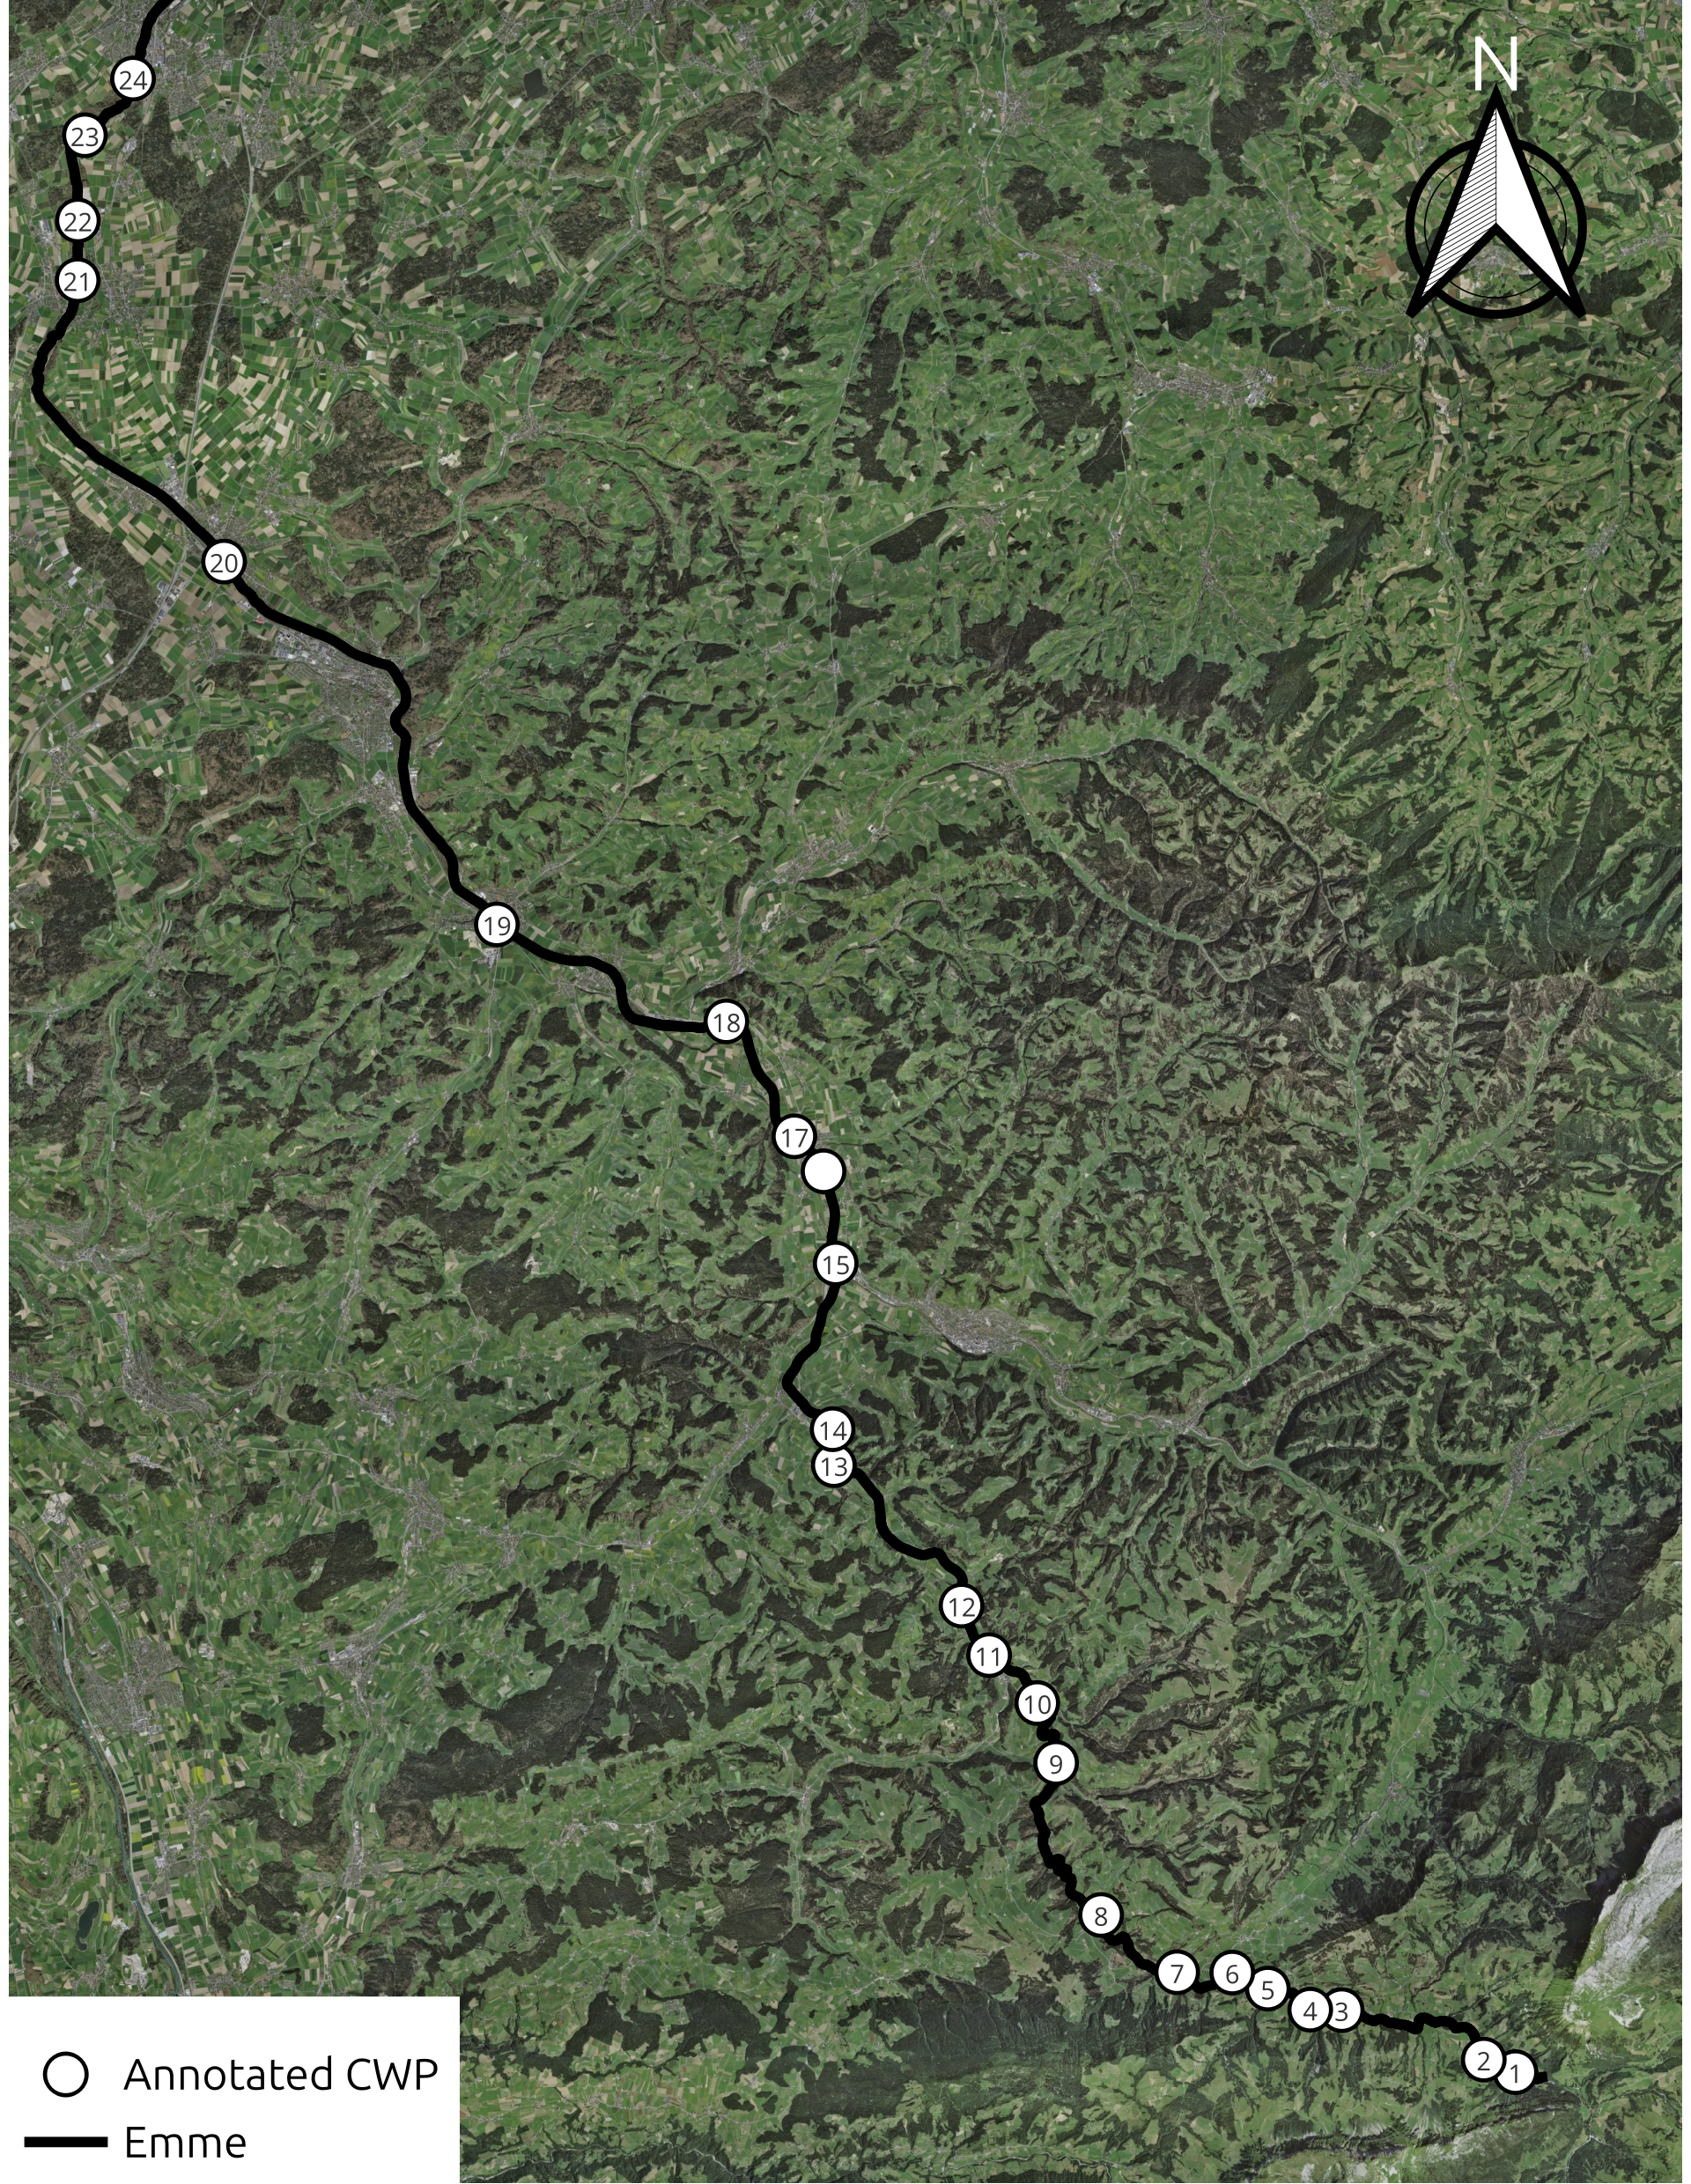
\includegraphics[width=\textwidth]{Bilder/annotated_cwp_locations.png}
	\caption{Annotated locations of cold water patches (CWP) in the Emme River.
		Each marker indicates the geographic position of a classified CWP. Background Image: Swissimage © Swisstopo
}
	\label{fig:cwp_locations_emme}
\end{figure}
\begin{figure}[p]
	\centering
	\vspace{0.5em}
	
	% Row 1
	\begin{subfigure}[t]{0.3\textwidth}
		\centering
		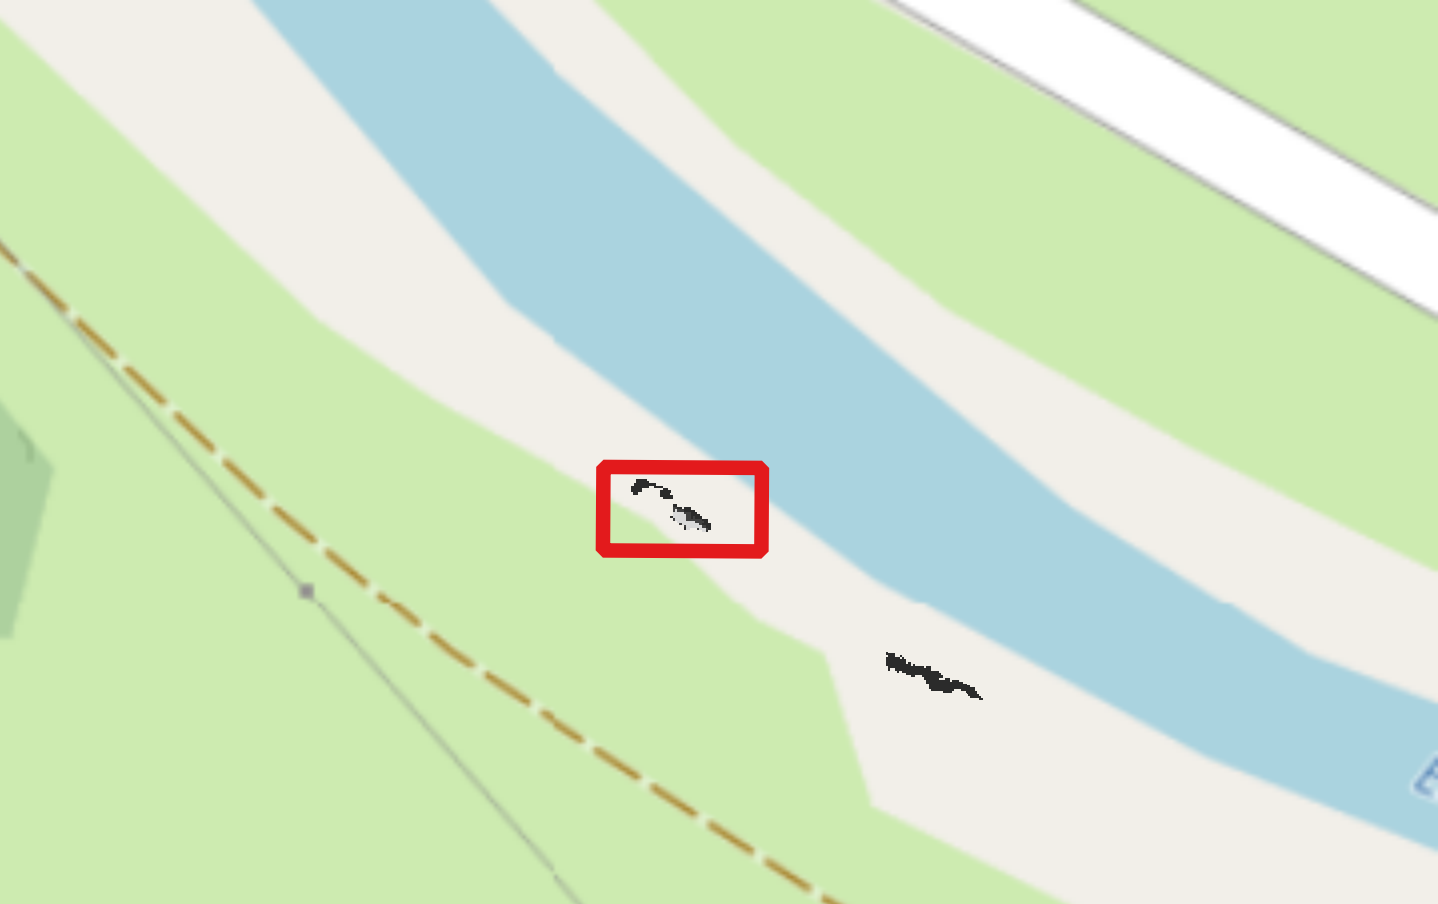
\includegraphics[width=\linewidth, height=3.5cm, keepaspectratio]{Bilder/cwp_images/1.png}
		\caption*{1}
	\end{subfigure}
	\hfill
	\begin{subfigure}[t]{0.3\textwidth}
		\centering
		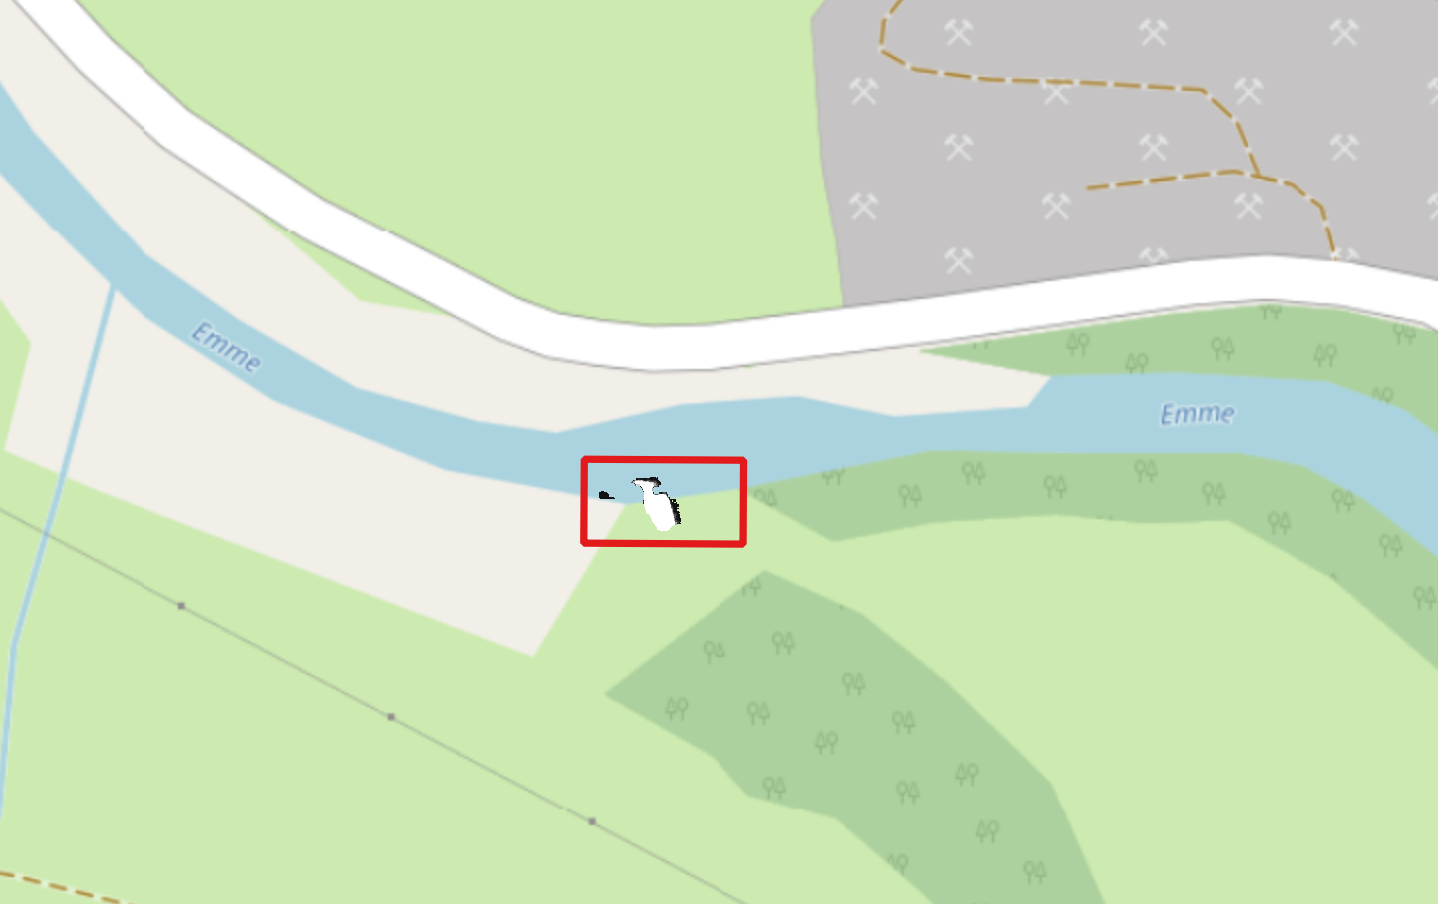
\includegraphics[width=\linewidth, height=3.5cm, keepaspectratio]{Bilder/cwp_images/2.png}
		\caption*{2}
	\end{subfigure}
	\hfill
	\begin{subfigure}[t]{0.3\textwidth}
		\centering
		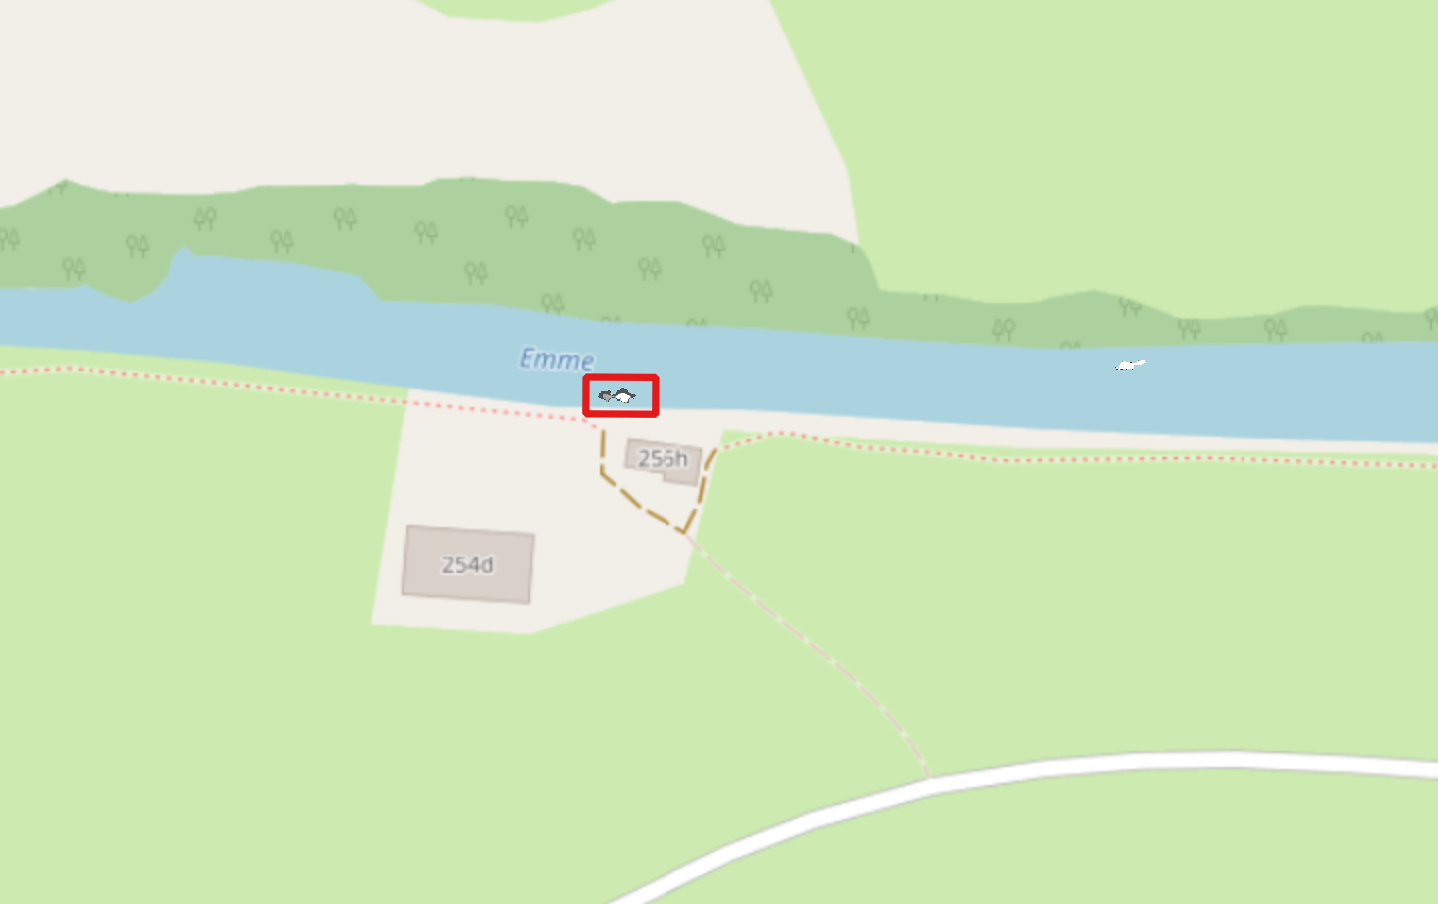
\includegraphics[width=\linewidth, height=3.5cm, keepaspectratio]{Bilder/cwp_images/3.png}
		\caption*{3}
	\end{subfigure}
	
	\vspace{1em}
	
	% Row 2
	\begin{subfigure}[t]{0.3\textwidth}
		\centering
		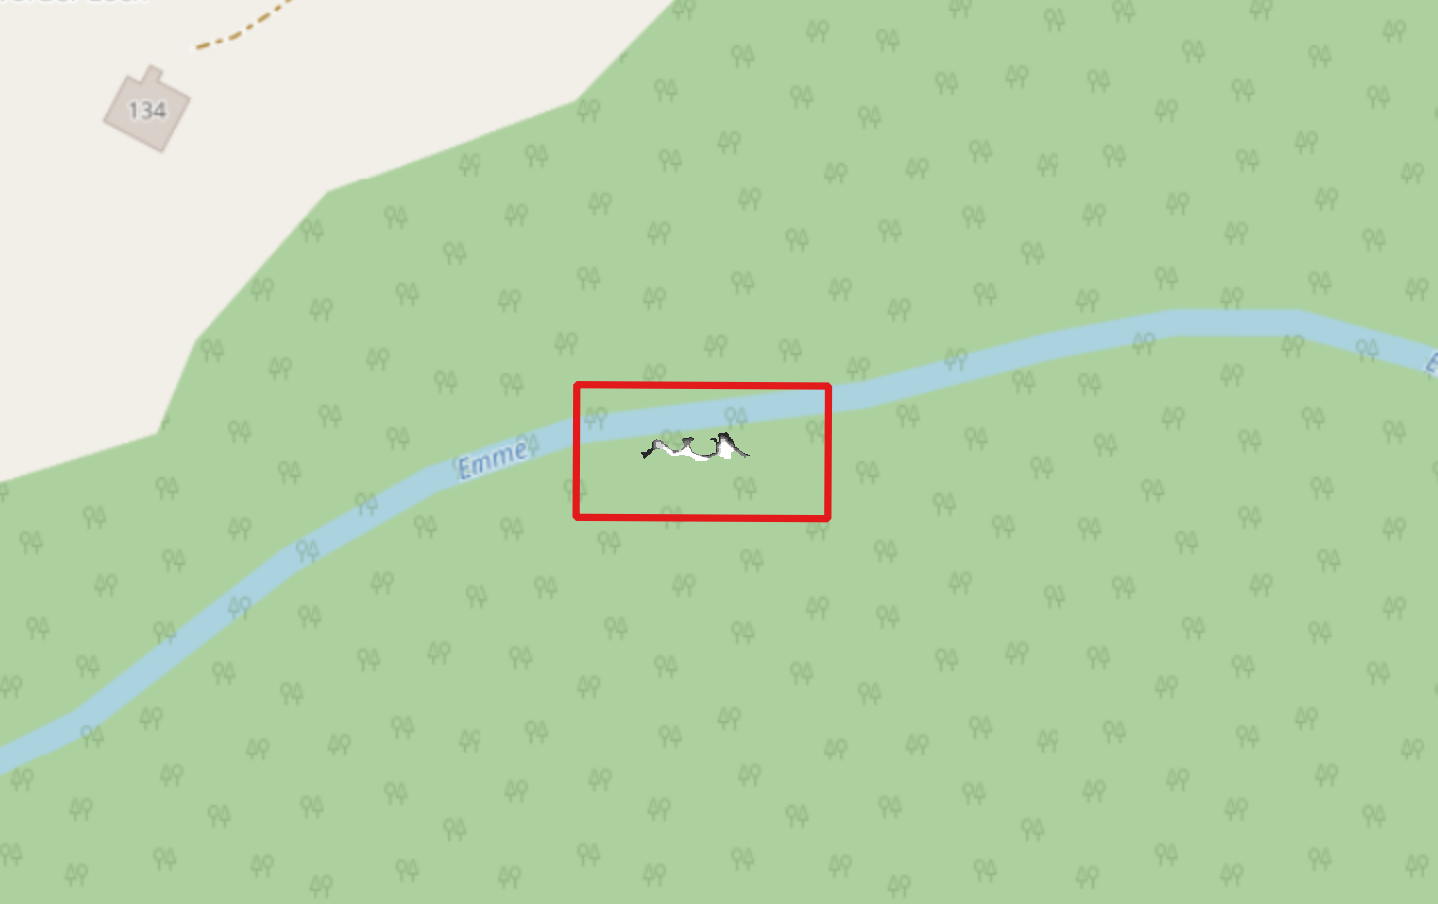
\includegraphics[width=\linewidth, height=3.5cm, keepaspectratio]{Bilder/cwp_images/5.png}
		\caption*{5}
	\end{subfigure}
	\hfill
	\begin{subfigure}[t]{0.3\textwidth}
		\centering
		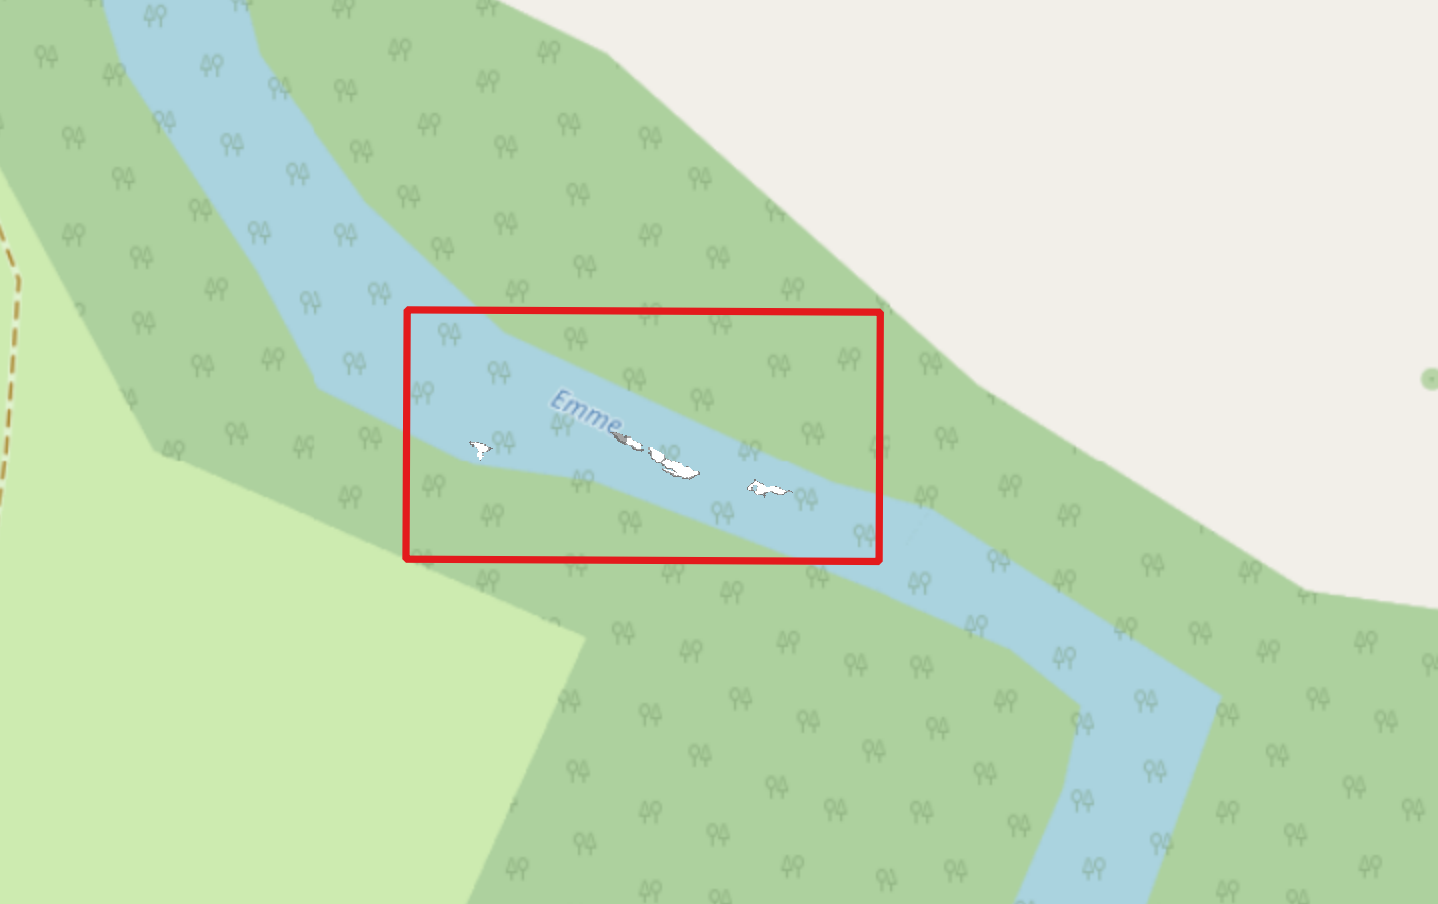
\includegraphics[width=\linewidth, height=3.5cm, keepaspectratio]{Bilder/cwp_images/8.png}
		\caption*{8}
	\end{subfigure}
	\hfill
	\begin{subfigure}[t]{0.3\textwidth}
		\centering
		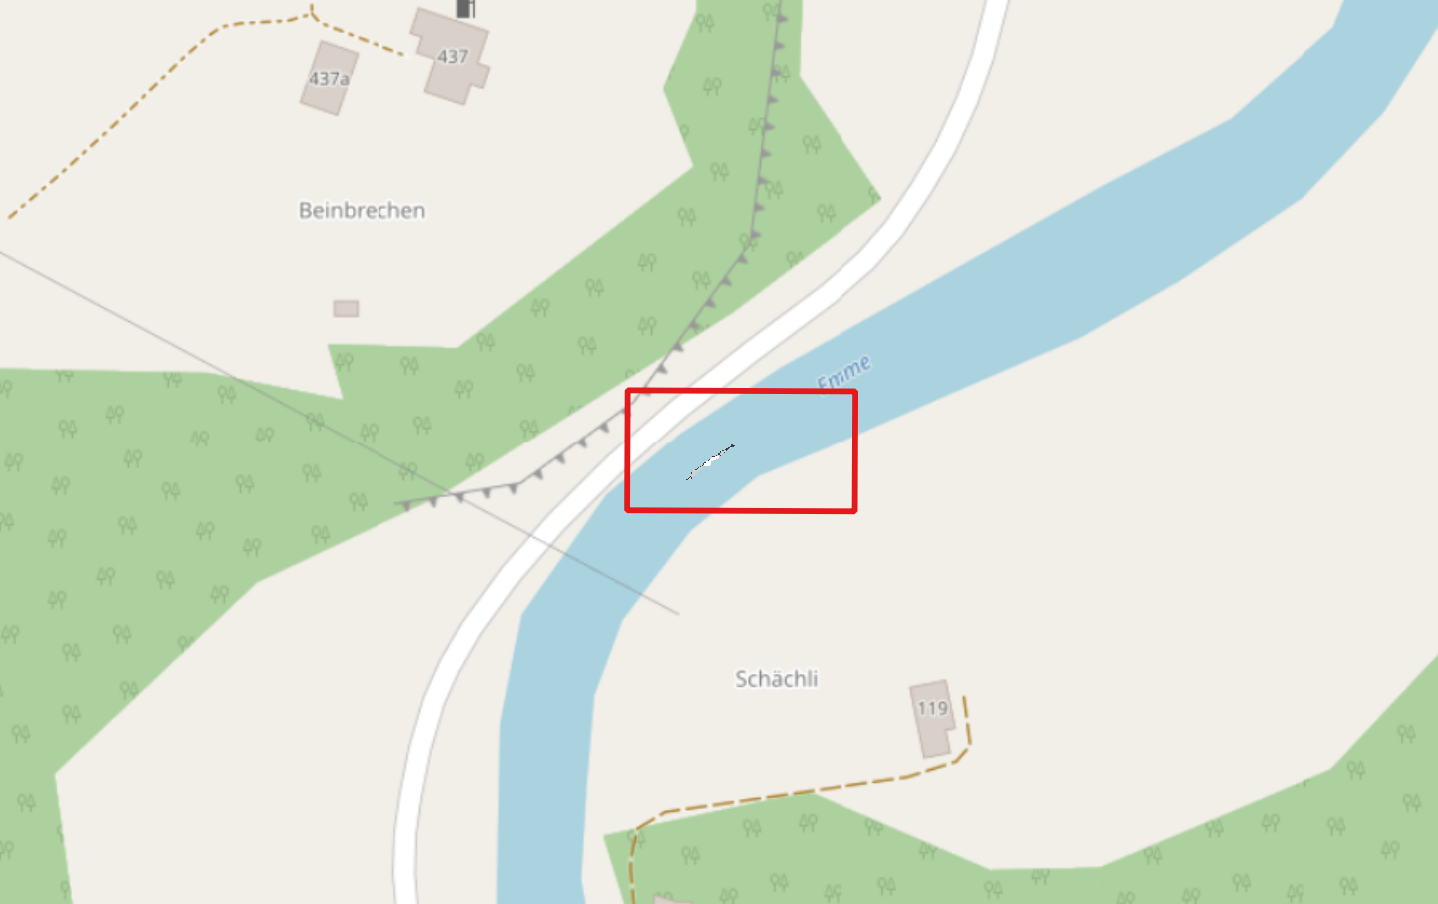
\includegraphics[width=\linewidth, height=3.5cm, keepaspectratio]{Bilder/cwp_images/9.png}
		\caption*{9}
	\end{subfigure}
	
	\vspace{1em}
	
	% Row 3
	\begin{subfigure}[t]{0.3\textwidth}
		\centering
		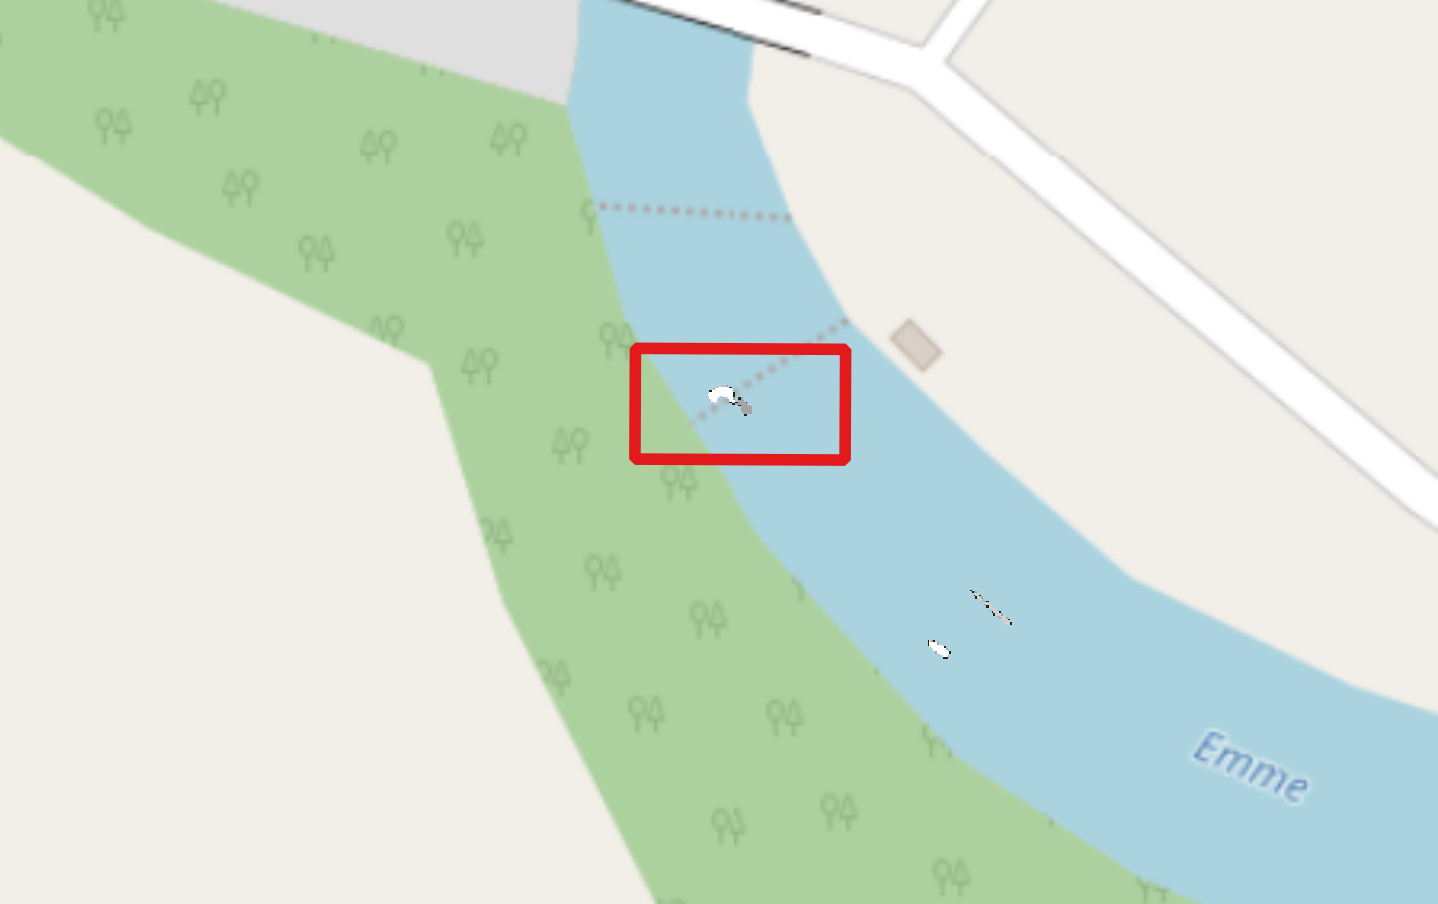
\includegraphics[width=\linewidth, height=3.5cm, keepaspectratio]{Bilder/cwp_images/10.png}
		\caption*{10}
	\end{subfigure}
	\hfill
	\begin{subfigure}[t]{0.3\textwidth}
		\centering
		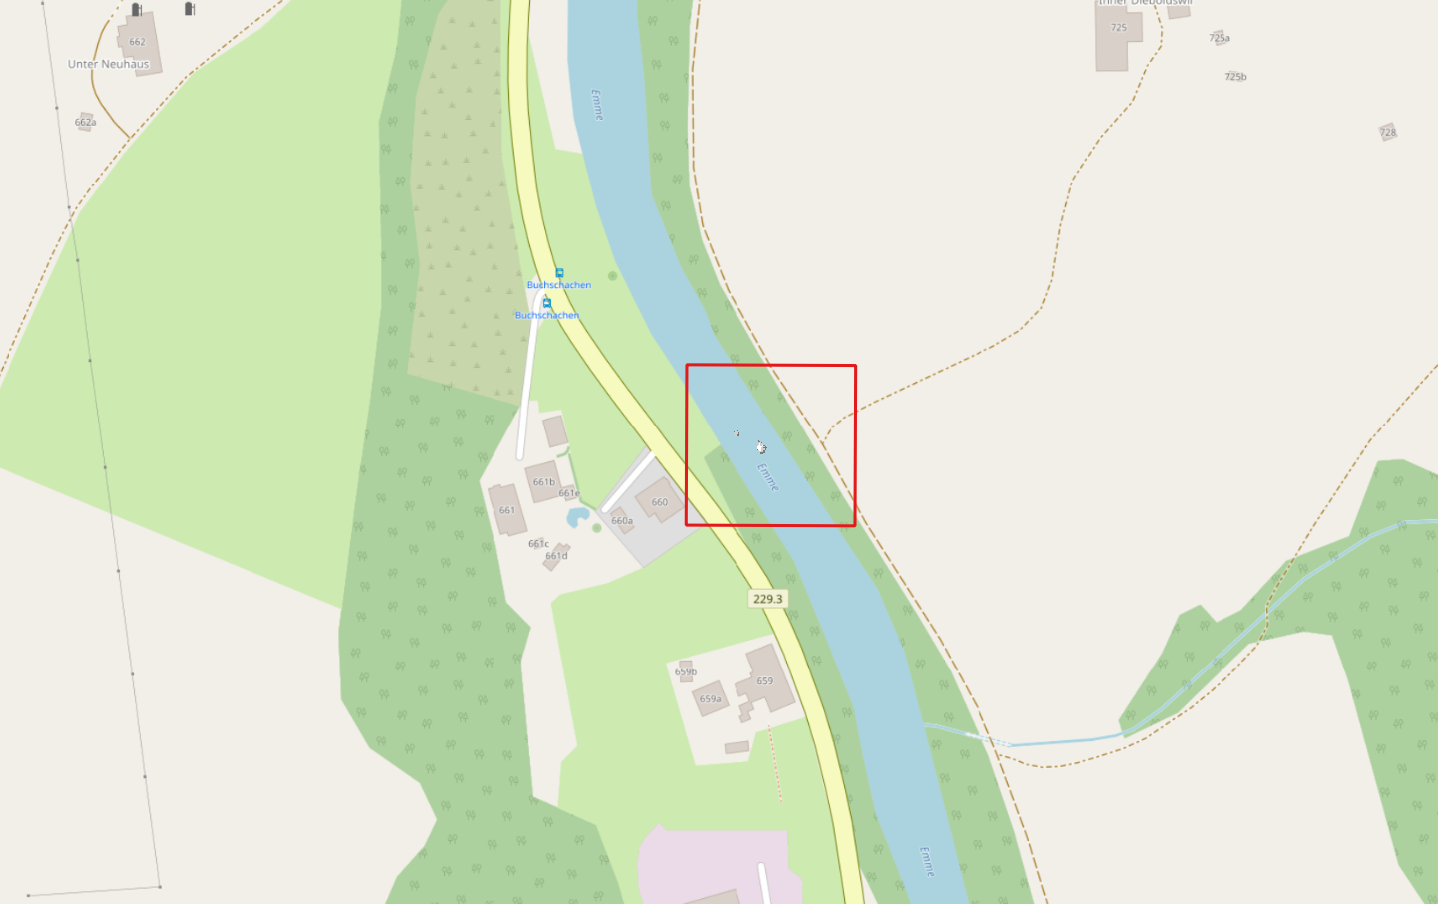
\includegraphics[width=\linewidth, height=3.5cm, keepaspectratio]{Bilder/cwp_images/12.png}
		\caption*{12}
	\end{subfigure}
	\hfill
	\begin{subfigure}[t]{0.3\textwidth}
		\centering
		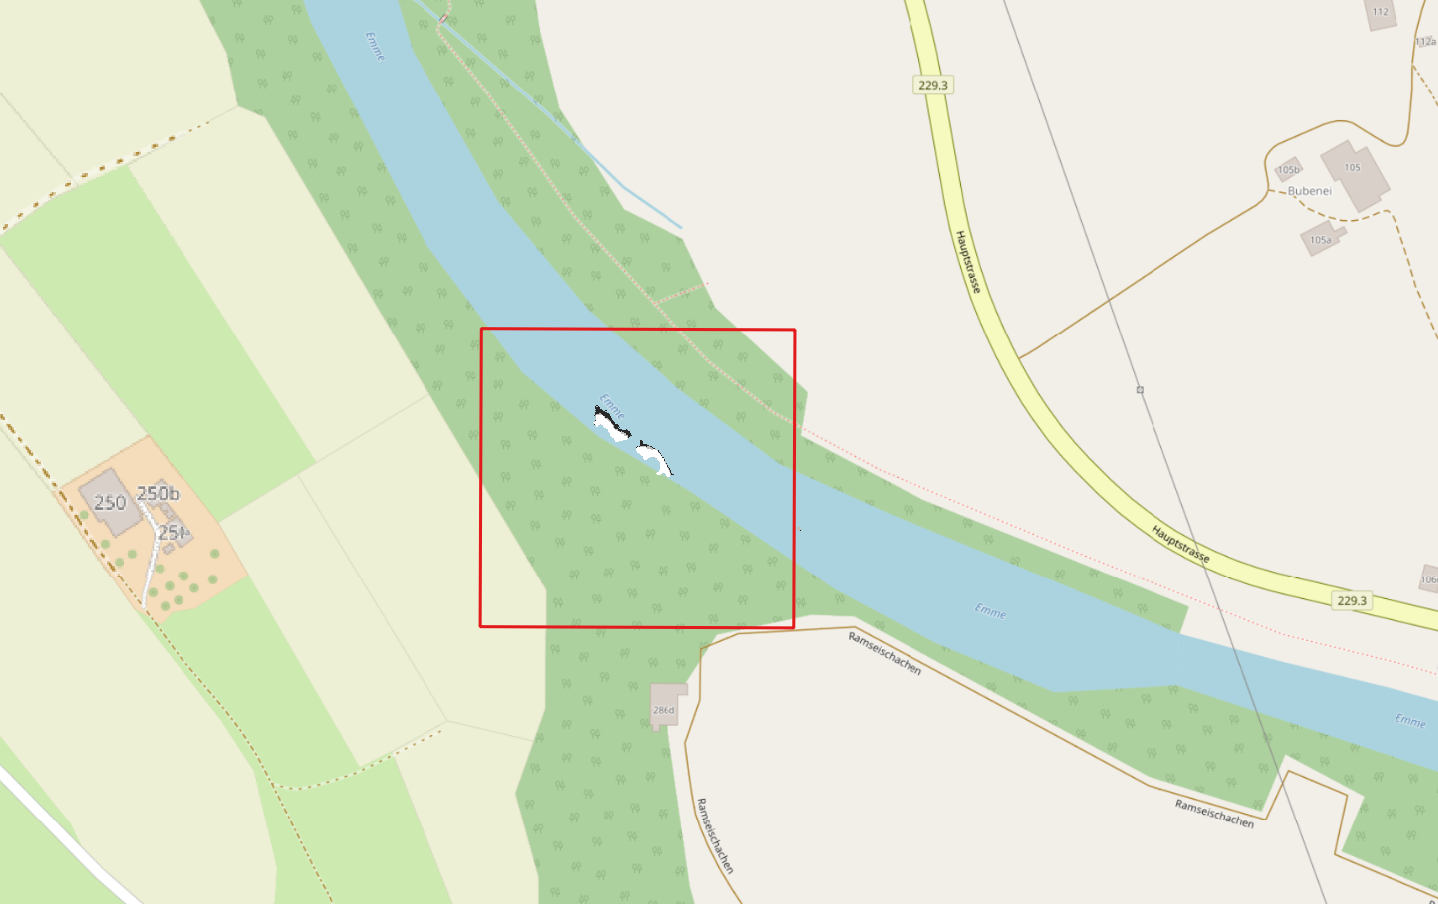
\includegraphics[width=\linewidth, height=3.5cm, keepaspectratio]{Bilder/cwp_images/13.png}
		\caption*{13}
	\end{subfigure}
	
	\vspace{1em}
	
	% Row 4
	\begin{subfigure}[t]{0.3\textwidth}
		\centering
		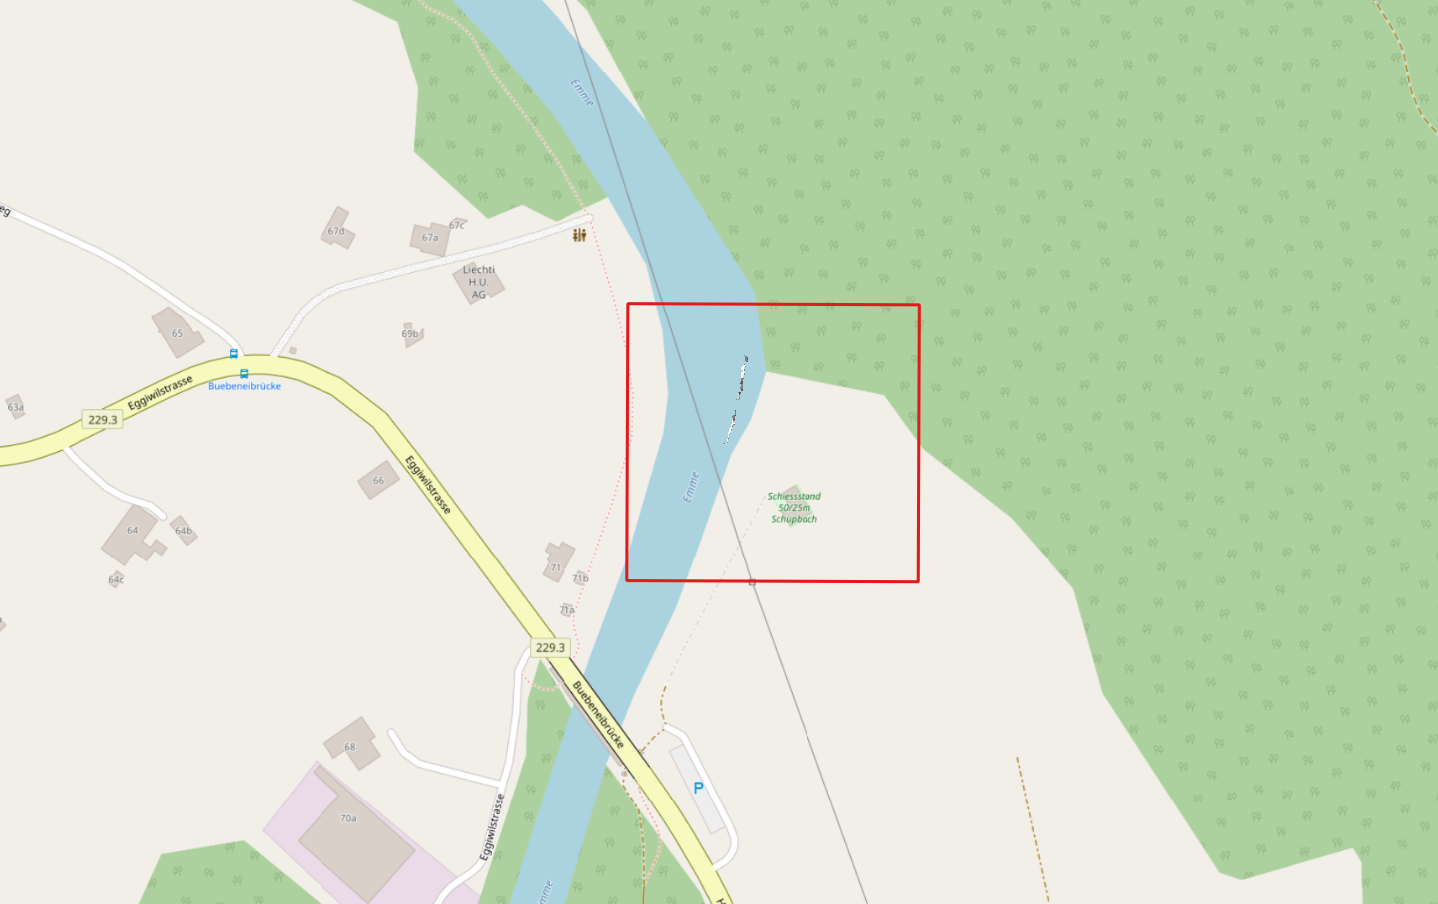
\includegraphics[width=\linewidth, height=3.5cm, keepaspectratio]{Bilder/cwp_images/14.png}
		\caption*{14}
	\end{subfigure}
	\hfill
	\begin{subfigure}[t]{0.3\textwidth}
		\centering
		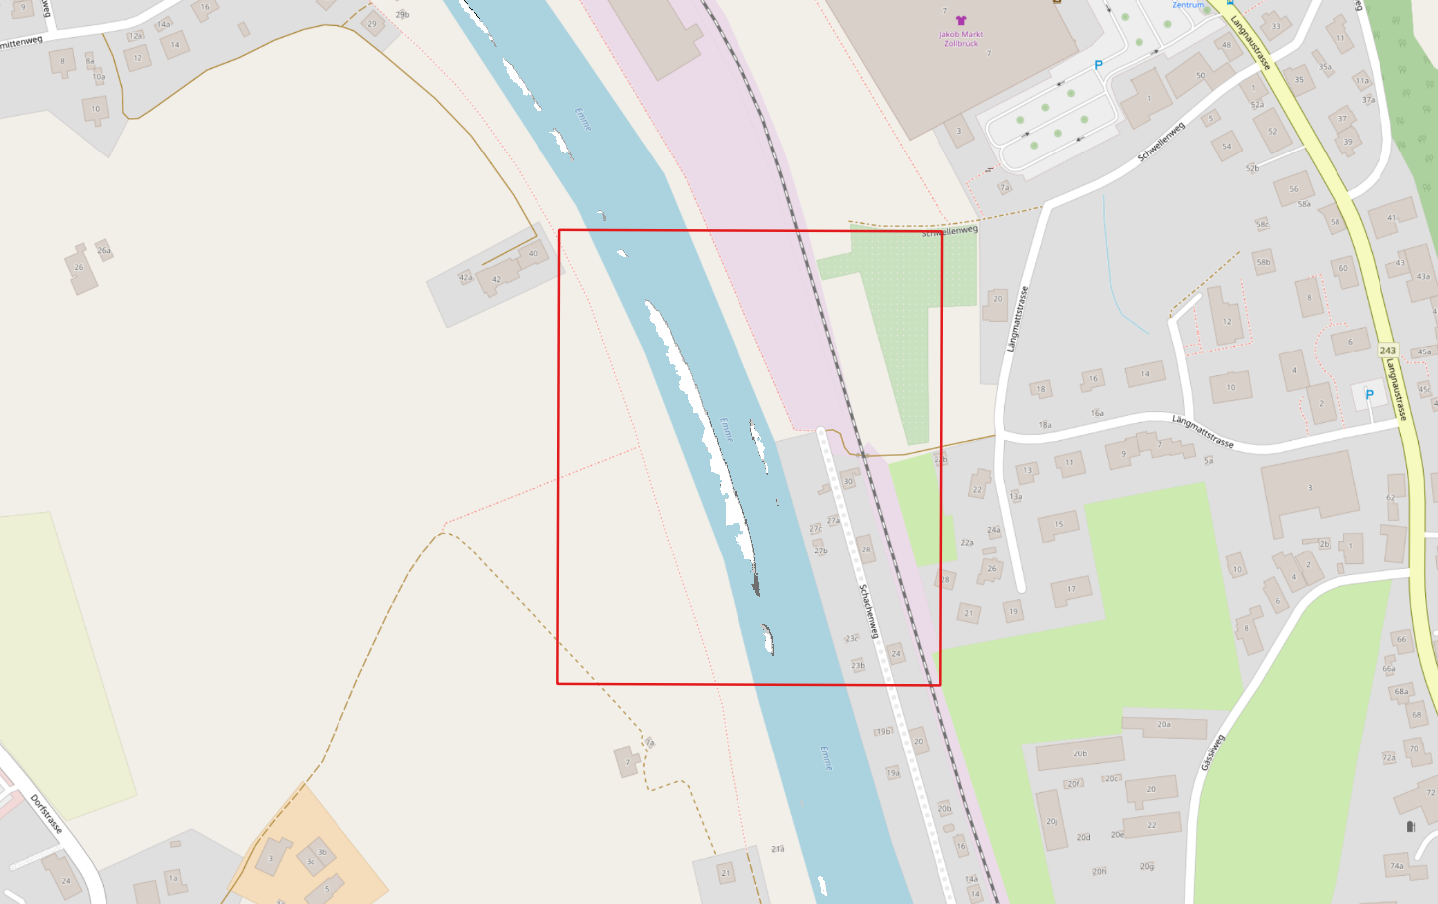
\includegraphics[width=\linewidth, height=3.5cm, keepaspectratio]{Bilder/cwp_images/16.png}
		\caption*{16}
	\end{subfigure}
	\hfill
	\begin{subfigure}[t]{0.3\textwidth}
		\centering
		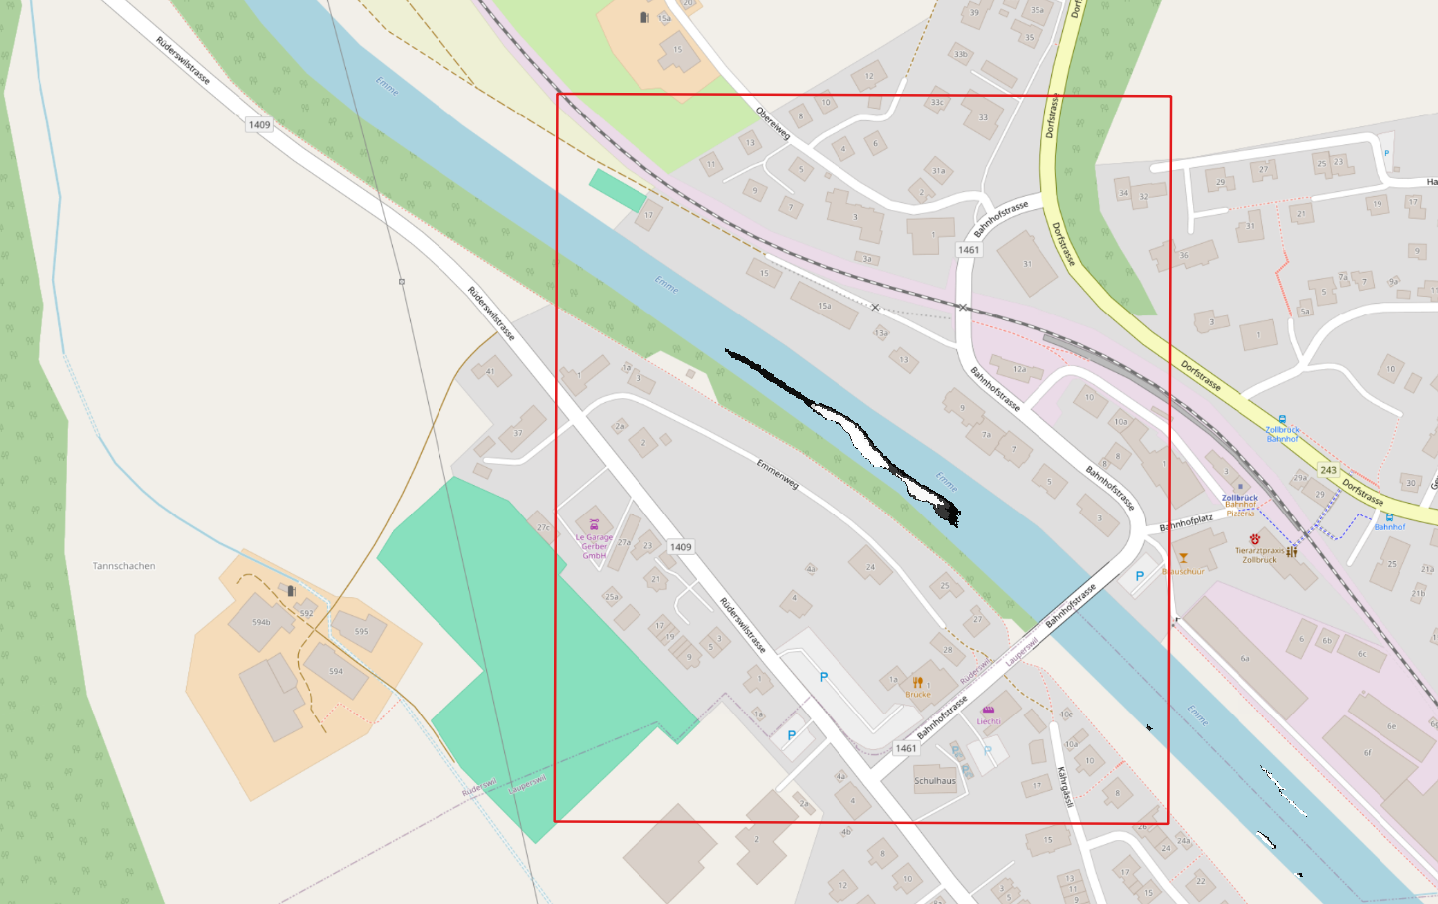
\includegraphics[width=\linewidth, height=3.5cm, keepaspectratio]{Bilder/cwp_images/17.png}
		\caption*{17}
	\end{subfigure}
	
	\vspace{1em}
	
% Row 5
\begin{subfigure}[t]{0.3\textwidth}
	\centering
	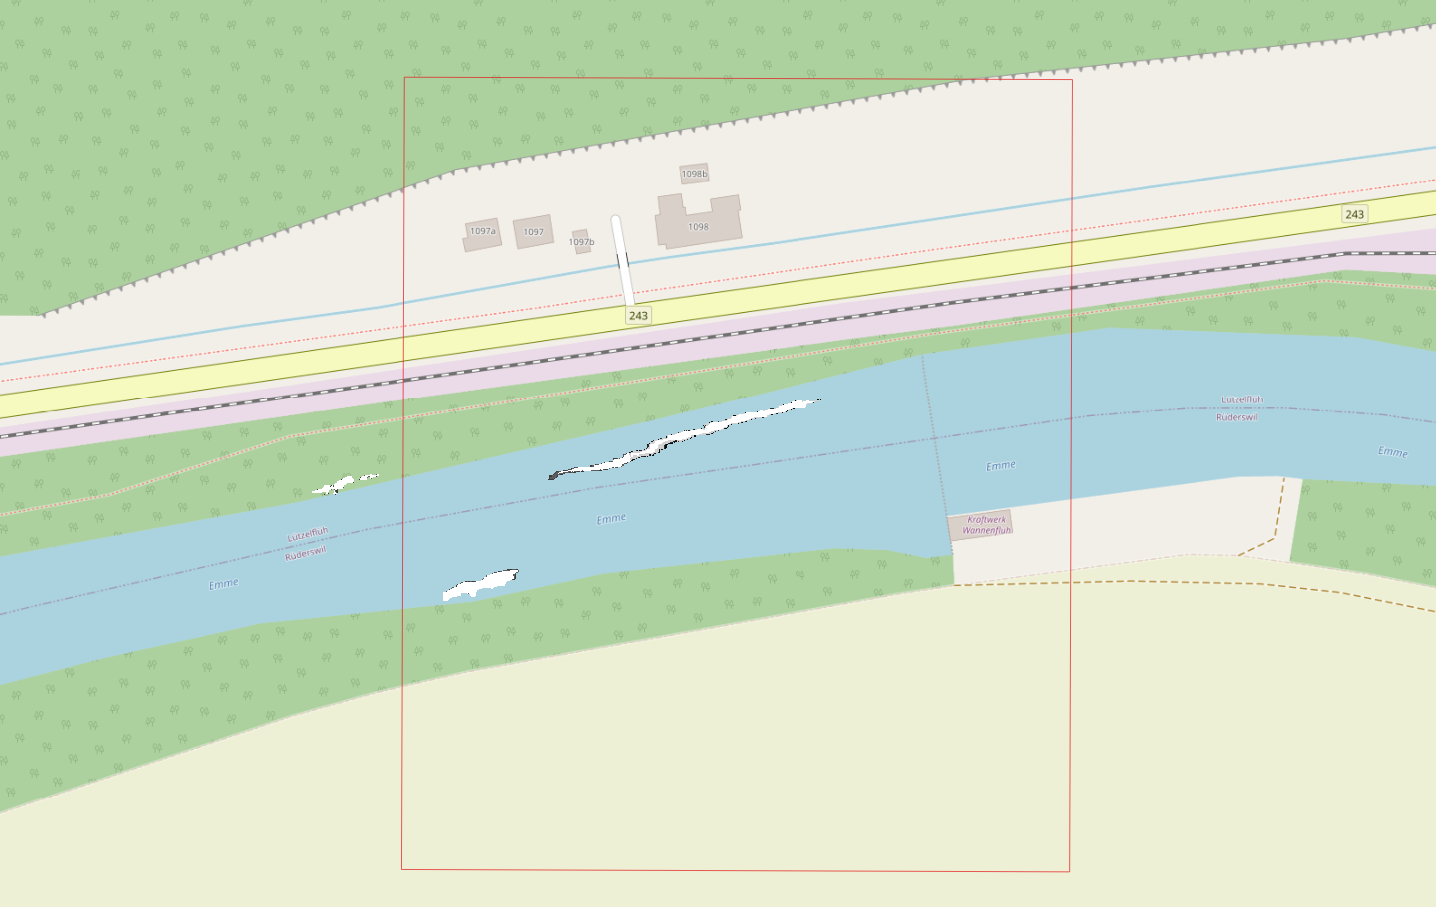
\includegraphics[width=\linewidth, height=3.5cm, keepaspectratio]{Bilder/cwp_images/18.png}
	\caption*{18}
\end{subfigure}
\hfill
\begin{subfigure}[t]{0.3\textwidth}
	\centering
	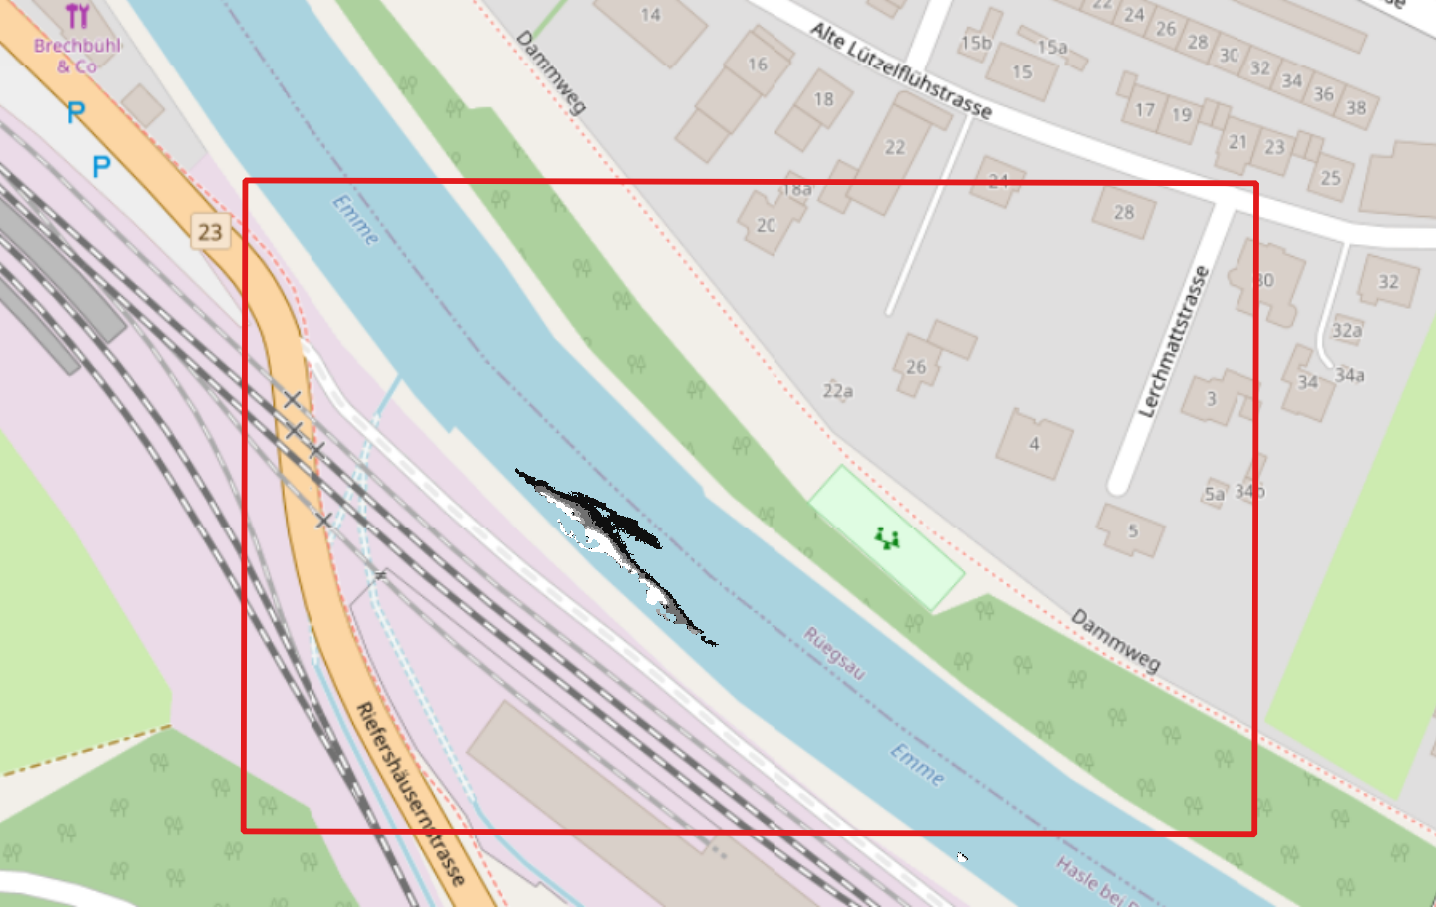
\includegraphics[width=\linewidth, height=3.5cm, keepaspectratio]{Bilder/cwp_images/19.png}
	\caption*{19}
\end{subfigure}
\hfill
\begin{subfigure}[t]{0.3\textwidth}
	\centering
	\phantom{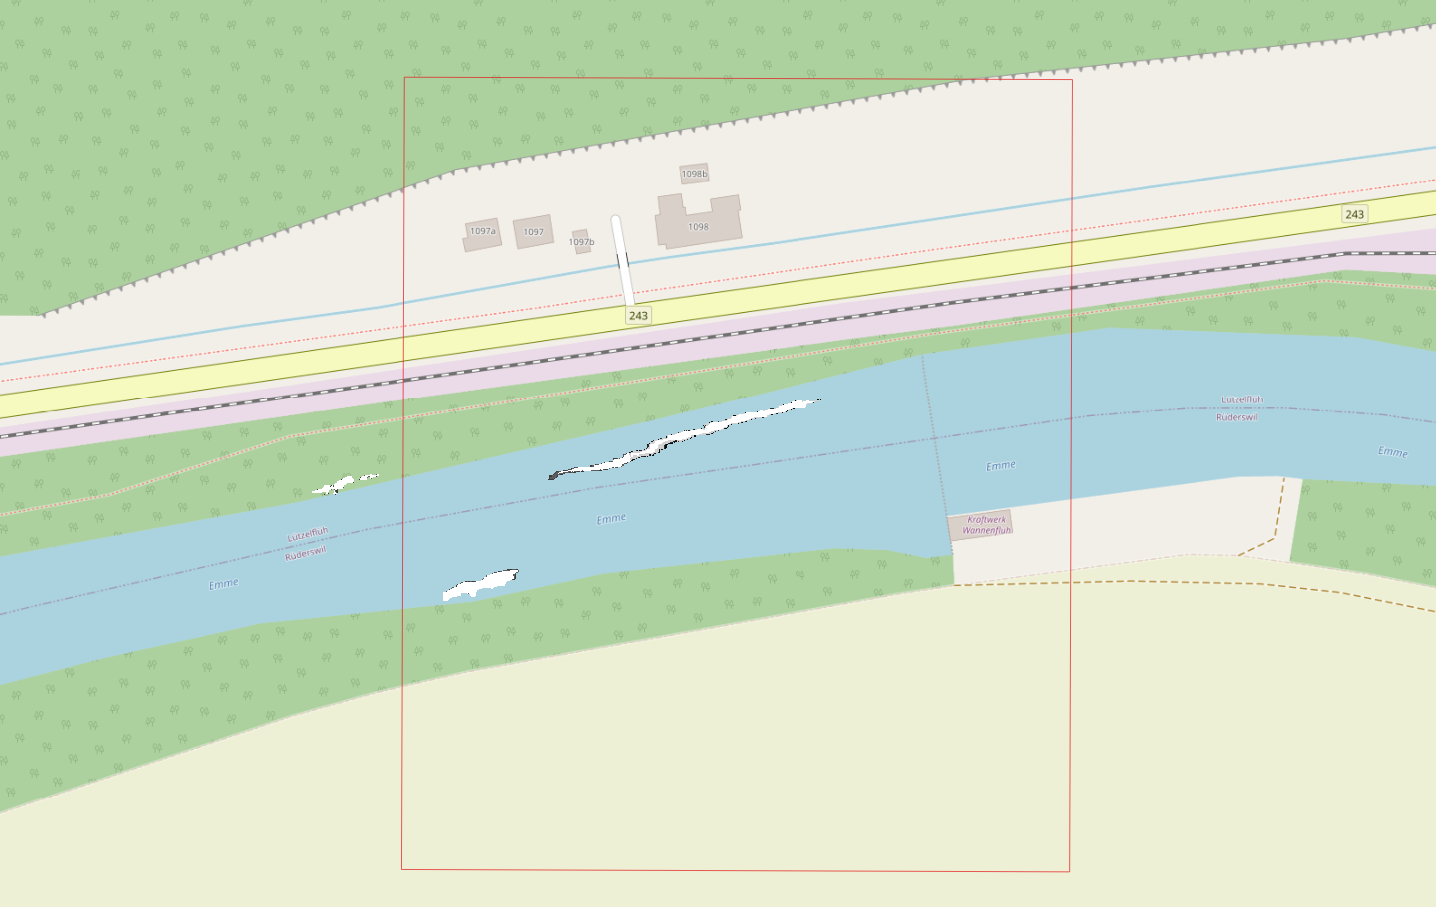
\includegraphics[width=\linewidth, height=3.5cm]{Bilder/cwp_images/18.png}}
\end{subfigure}
	
	\caption{Catalogue of non-tributary-caused cold-water patches ($N = 14$). 
		Each patch is shown as a detection frequency raster excerpt.}
	\label{fig:cwp_catalogue_nt}
\end{figure}

\begin{figure}[p]
	\centering
	\vspace{0.5em}
	
	% Row 1
	\begin{subfigure}[t]{0.3\textwidth}
		\centering
		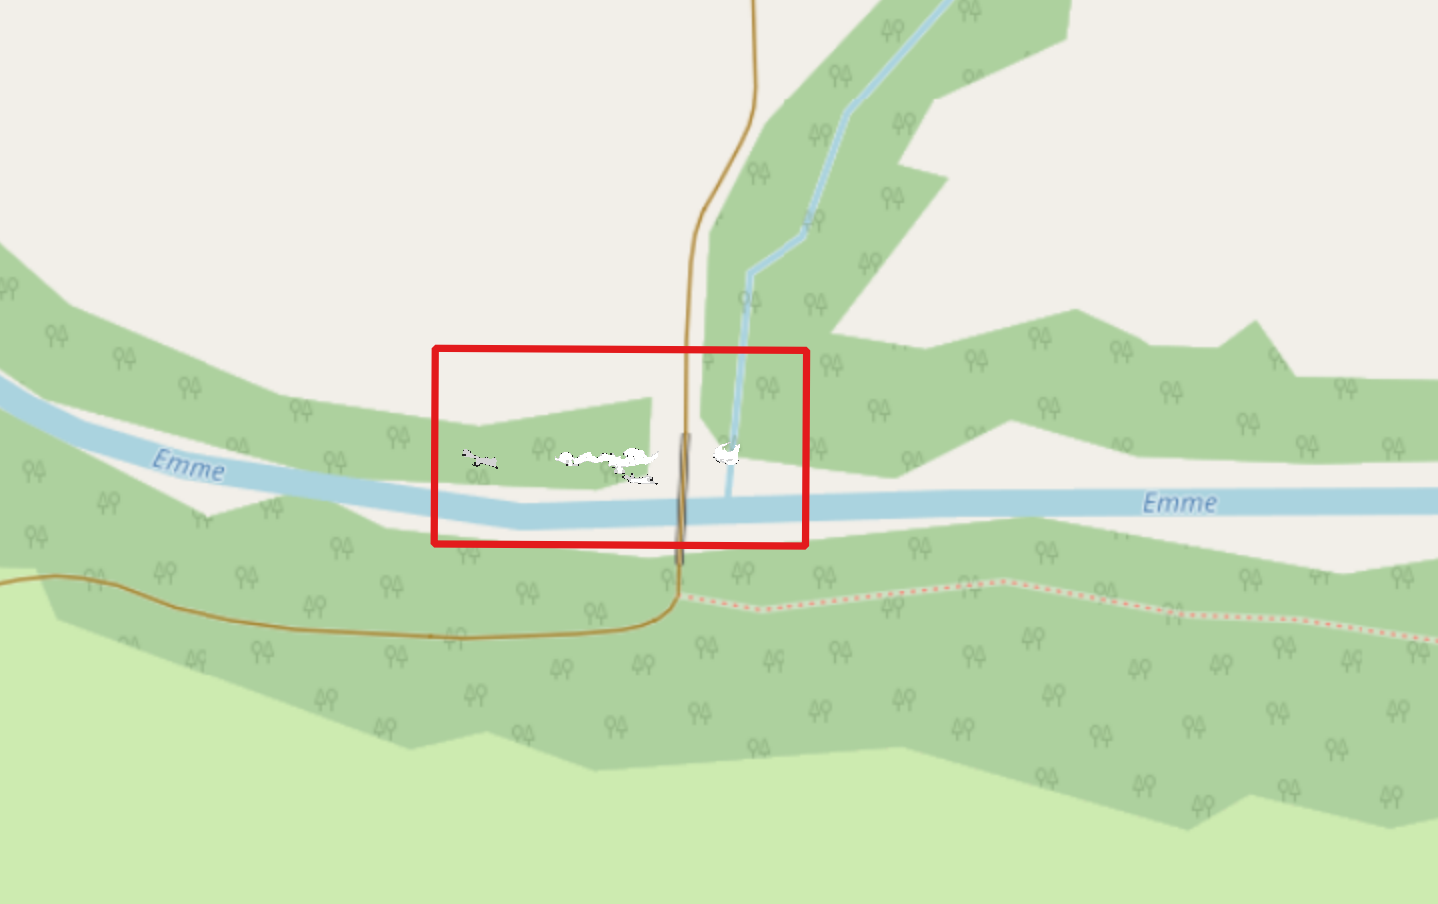
\includegraphics[width=\linewidth, height=4cm, keepaspectratio]{Bilder/cwp_images/4.png}
		\caption*{4}
	\end{subfigure}
	\hfill
	\begin{subfigure}[t]{0.3\textwidth}
		\centering
		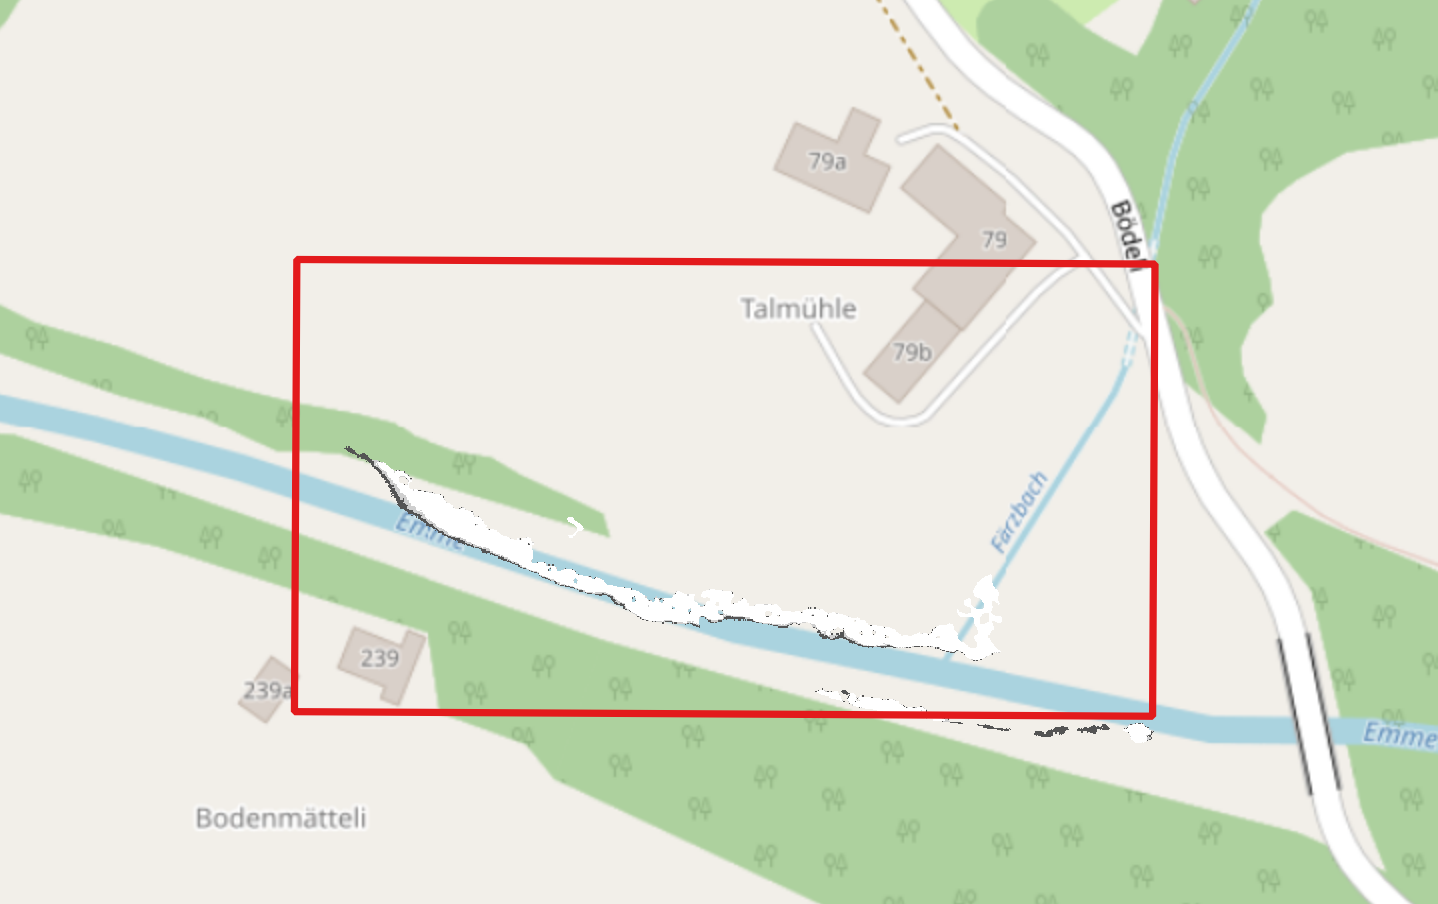
\includegraphics[width=\linewidth, height=4cm, keepaspectratio]{Bilder/cwp_images/6.png}
		\caption*{6}
	\end{subfigure}
	\hfill
	\begin{subfigure}[t]{0.3\textwidth}
		\centering
		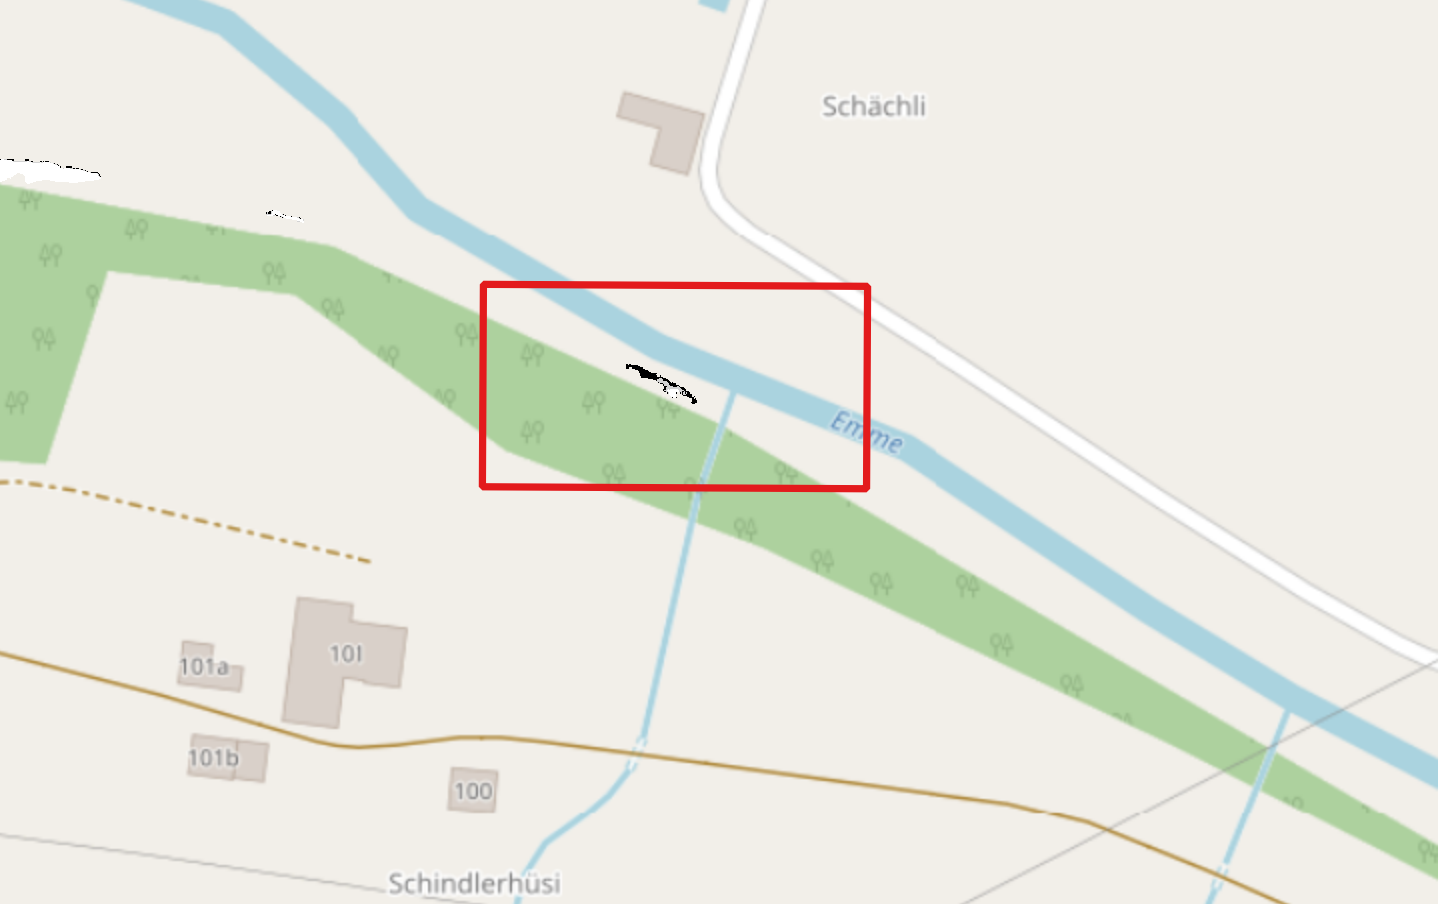
\includegraphics[width=\linewidth, height=4cm, keepaspectratio]{Bilder/cwp_images/7.png}
		\caption*{7}
	\end{subfigure}
	
	\vspace{1em}
	
	% Row 2
	\begin{subfigure}[t]{0.3\textwidth}
		\centering
		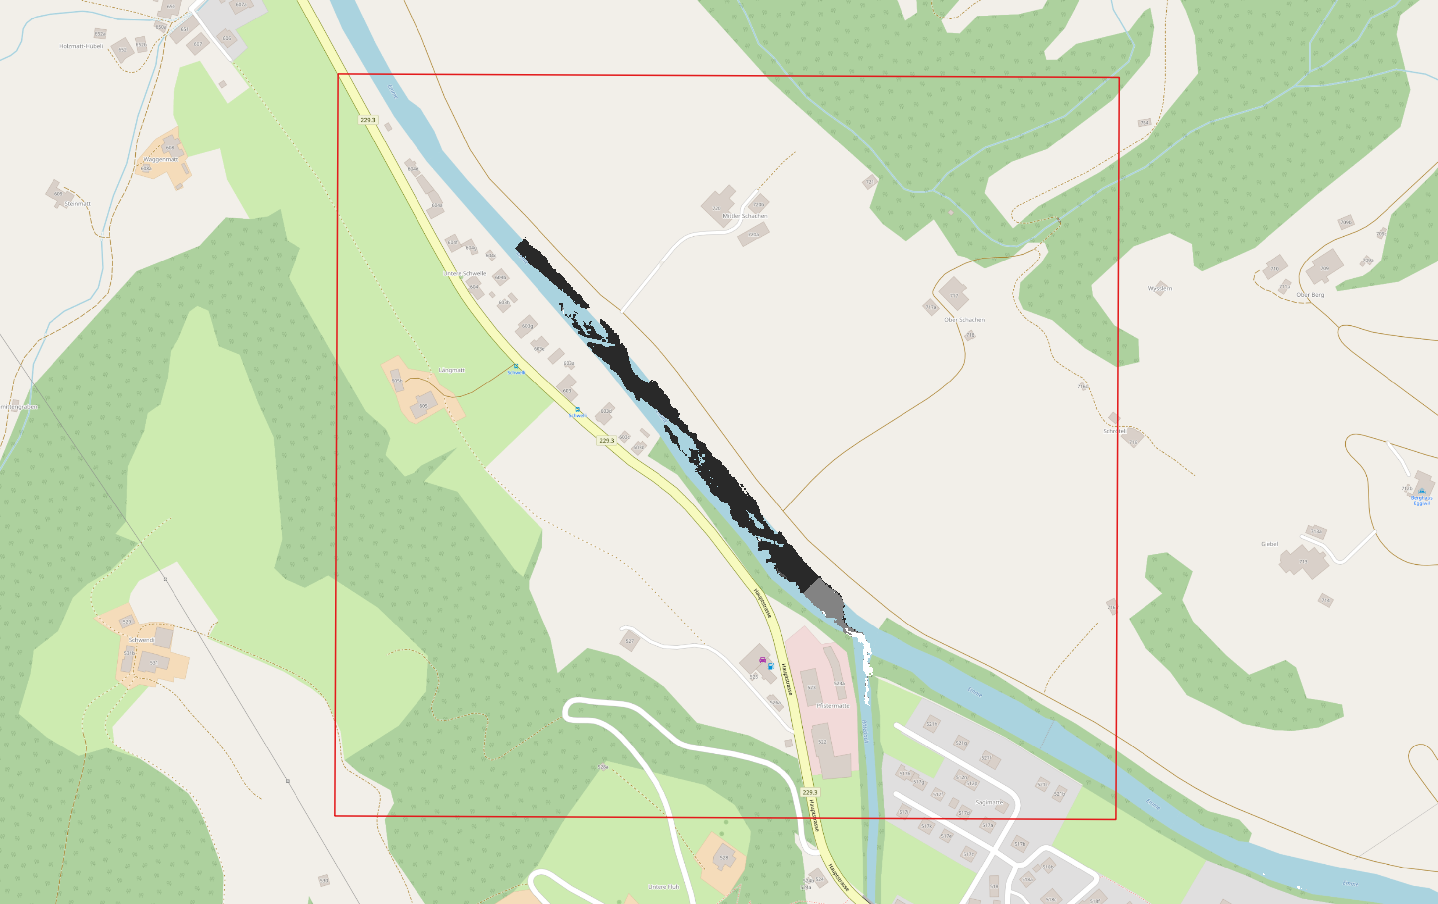
\includegraphics[width=\linewidth, height=4cm, keepaspectratio]{Bilder/cwp_images/11.png}
		\caption*{11}
	\end{subfigure}
	\hfill
	\begin{subfigure}[t]{0.3\textwidth}
		\centering
		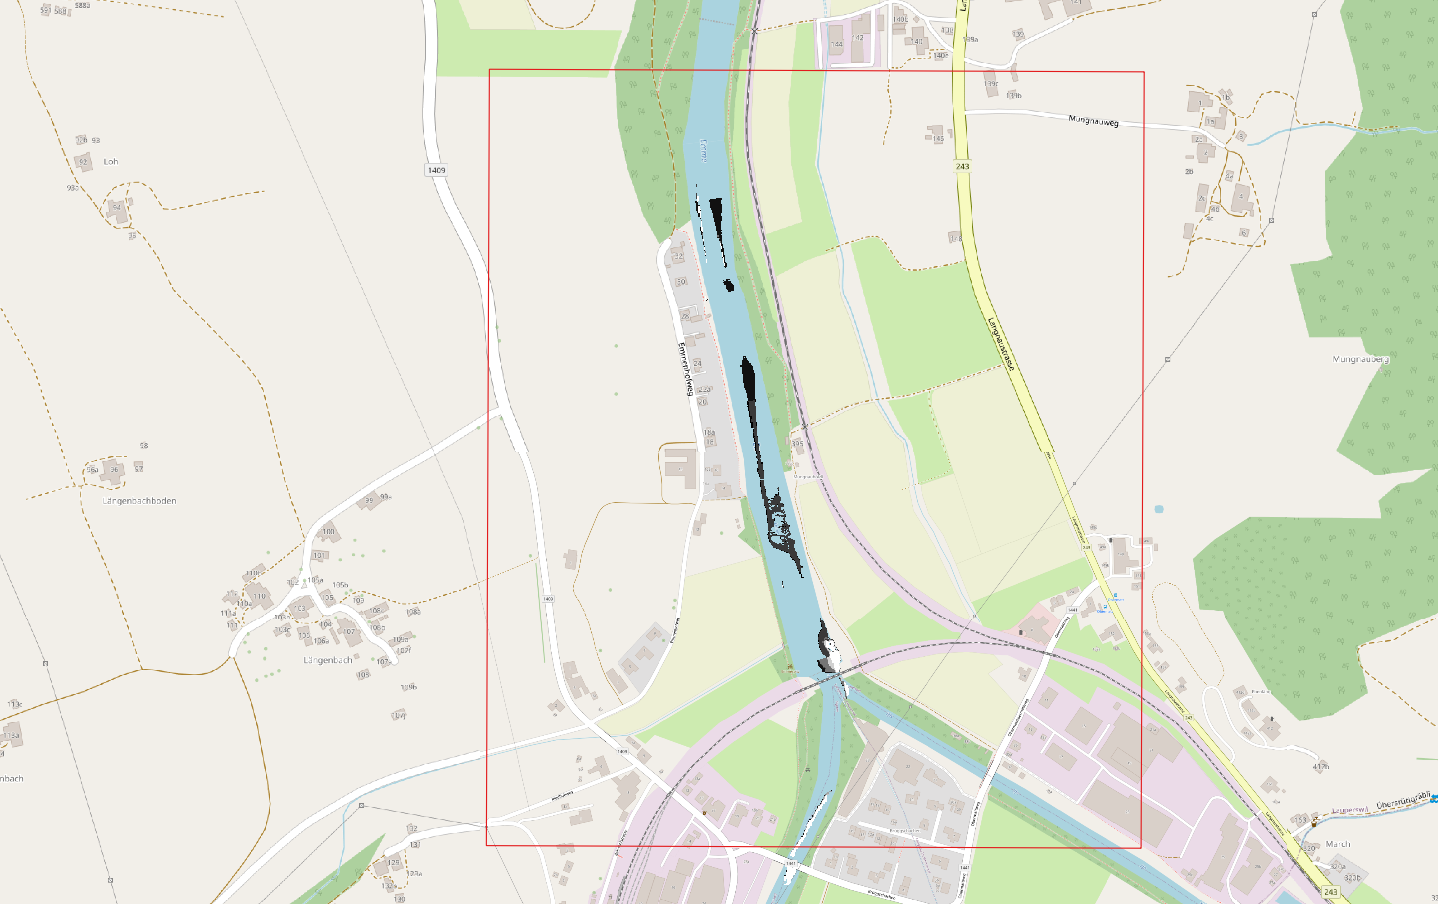
\includegraphics[width=\linewidth, height=4cm, keepaspectratio]{Bilder/cwp_images/15.png}
		\caption*{15}
	\end{subfigure}
	\hfill
	\begin{subfigure}[t]{0.3\textwidth}
		\centering
		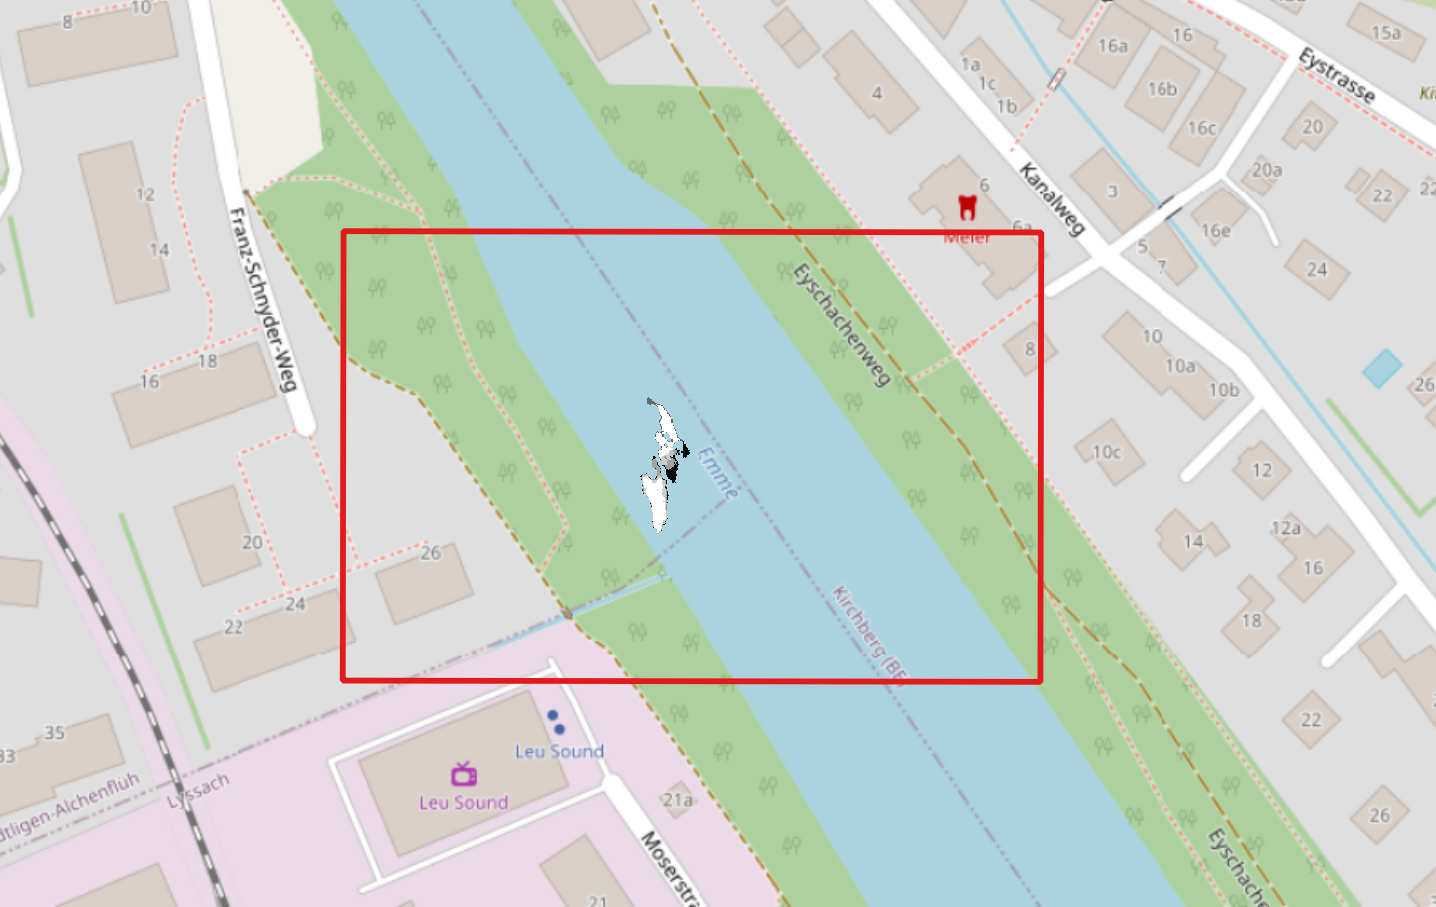
\includegraphics[width=\linewidth, height=4cm, keepaspectratio]{Bilder/cwp_images/20.png}
		\caption*{20}
	\end{subfigure}
	
	\vspace{1em}
	
	% Row 3
	\begin{subfigure}[t]{0.3\textwidth}
		\centering
		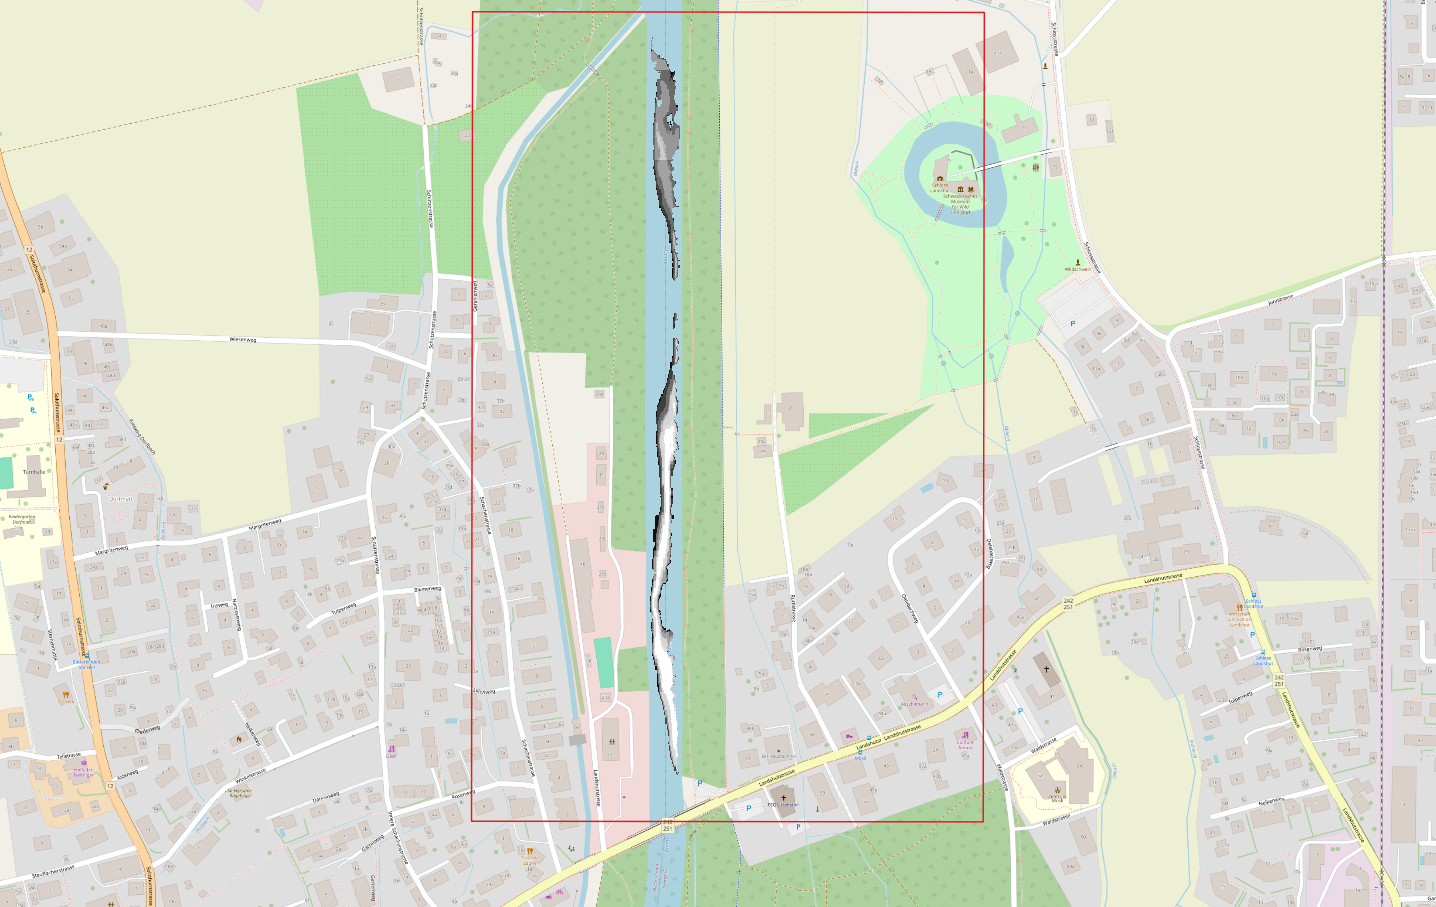
\includegraphics[width=\linewidth, height=4cm, keepaspectratio]{Bilder/cwp_images/21.png}
		\caption*{21}
	\end{subfigure}
	\hfill
	\begin{subfigure}[t]{0.3\textwidth}
		\centering
		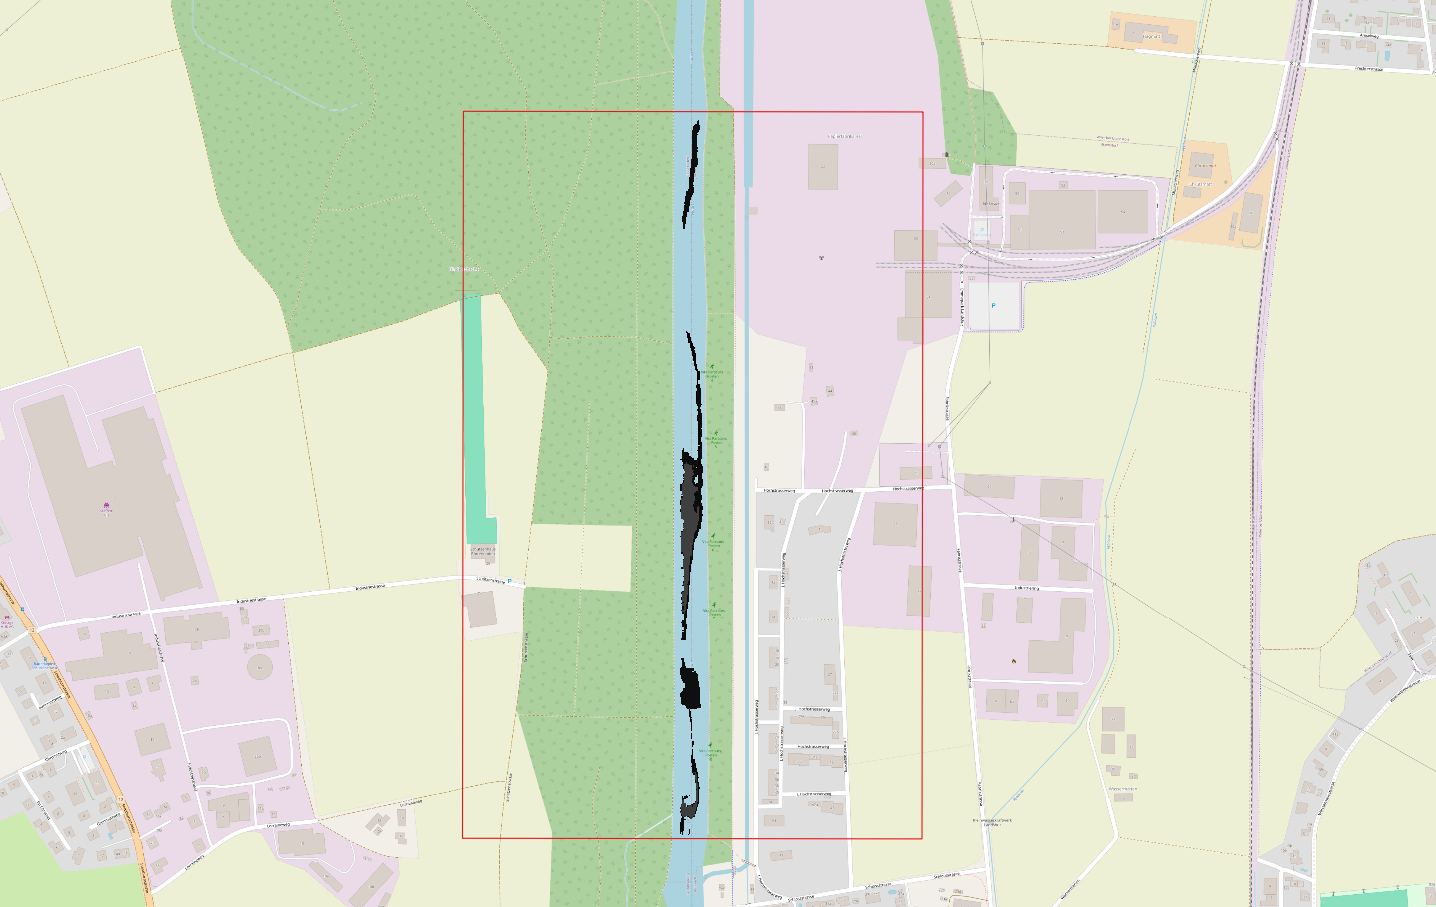
\includegraphics[width=\linewidth, height=4cm, keepaspectratio]{Bilder/cwp_images/22.png}
		\caption*{22}
	\end{subfigure}
	\hfill
	\begin{subfigure}[t]{0.3\textwidth}
		\centering
		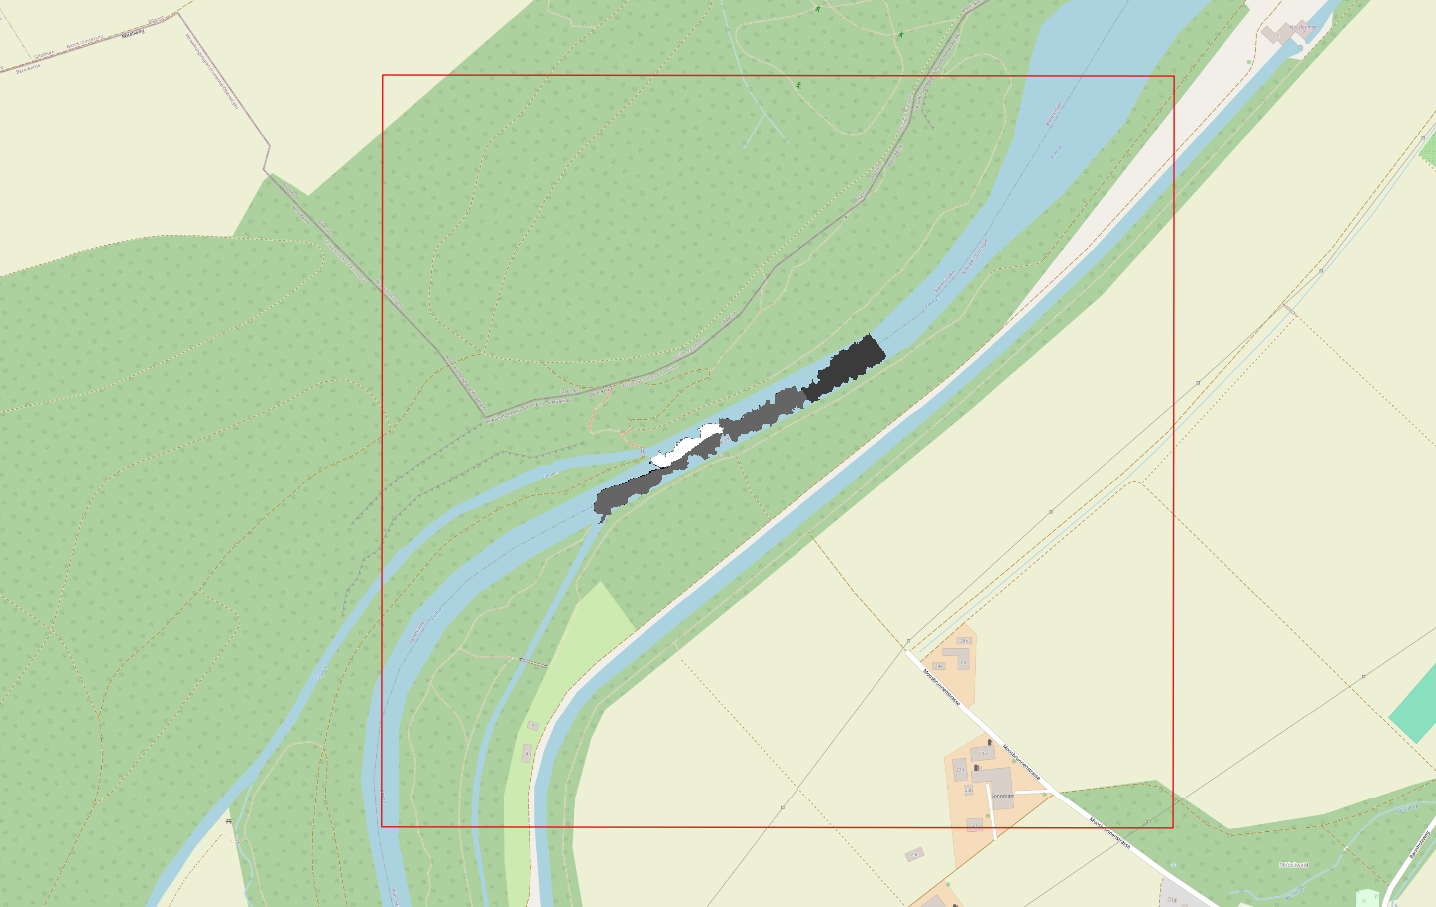
\includegraphics[width=\linewidth, height=4cm, keepaspectratio]{Bilder/cwp_images/23.png}
		\caption*{23}
	\end{subfigure}
	
	\vspace{1em}
	
	% Row 4
	\begin{subfigure}[t]{0.3\textwidth}
		\centering
		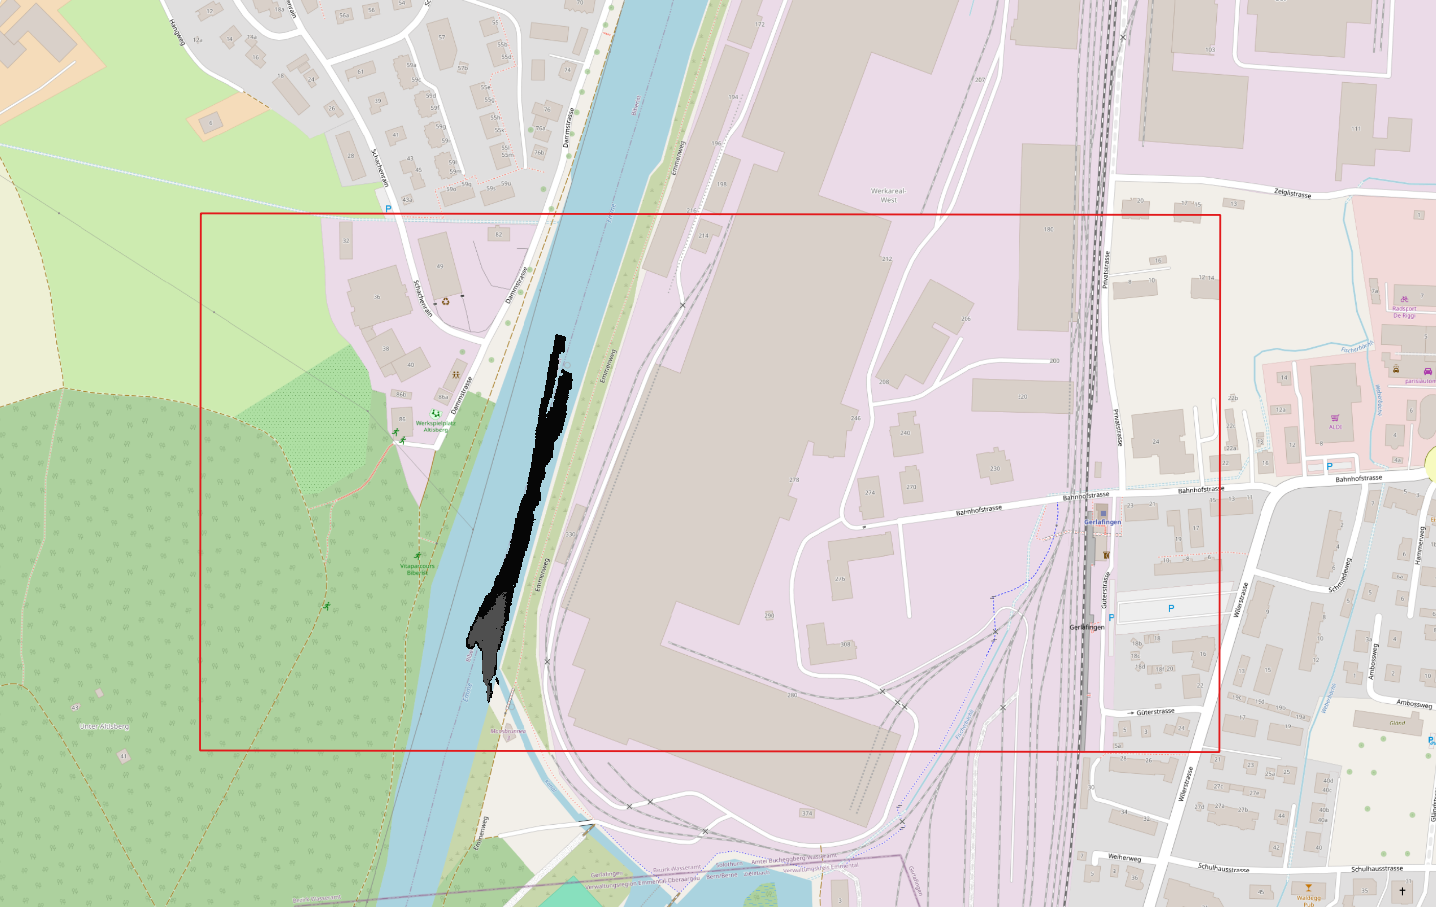
\includegraphics[width=\linewidth, height=4cm, keepaspectratio]{Bilder/cwp_images/24.png}
		\caption*{24}
	\end{subfigure}
	\hfill
	\begin{subfigure}[t]{0.3\textwidth}
		\centering
		% empty slot
	\end{subfigure}
	\hfill
	\begin{subfigure}[t]{0.3\textwidth}
		\centering
		% empty slot
	\end{subfigure}
	
	\caption{Catalogue of tributary-caused cold-water patches ($N = 10$). 
		Each patch is shown as a detection frequency raster excerpt.}
	\label{fig:cwp_catalogue_t}
\end{figure}

\section*{Appendix B: Statement of Reproducibility}

The complete R code associated with this thesis is available at:\\
\url{https://github.com/duerieti/Sensitivity-Analysis-of-a-TIR-Based-CWP-Detection-Algorithm}


\section*{Appendix C: List of Generative AI Systems}

The following generative AI systems and AI-assisted tools were utilized in the 
context of this work:

\begin{table}[H]
	\centering
	\begin{tabular}{@{} p{2.5cm} p{3.5cm} p{7cm} @{}}
		\toprule
		\textbf{System / Tool} & \textbf{Provider \& Version} & 
		\textbf{Purpose of Use} \\
		\midrule
		Claude Sonnet 4.6 & Anthropic (2026) \newline Version Sonnet 4.6 &
		\begin{itemize}[noitemsep, topsep=0pt, leftmargin=*]
			\item Stylistic improvement of text
			\item Spelling correction
			\item Code debugging and coding assistance (no agentic coding)
			\item \LaTeX{} assistant (debugging and formatting)
			\item Finding relevant literature
		\end{itemize} \\
		\addlinespace
		Claude Opus 4.6 & Anthropic (2026) \newline Version Opus 4.6 &
		\begin{itemize}[noitemsep, topsep=0pt, leftmargin=*]
			\item Complex debugging tasks
			\item Complex writing assistance tasks such as assuring 
			cross-chapter naming consistency
		\end{itemize} \\
		\bottomrule
	\end{tabular}
\end{table}

\vspace{0.5em}
\noindent\textit{Note:} The author assumes full responsibility for all generated 
content, its accuracy, and compliance with the standards of scientific integrity.
	
\end{document}